\documentclass[twoside]{book}

% Packages required by doxygen
\usepackage{fixltx2e}
\usepackage{calc}
\usepackage{doxygen}
\usepackage[export]{adjustbox} % also loads graphicx
\usepackage{graphicx}
\usepackage[utf8]{inputenc}
\usepackage{makeidx}
\usepackage{multicol}
\usepackage{multirow}
\PassOptionsToPackage{warn}{textcomp}
\usepackage{textcomp}
\usepackage[nointegrals]{wasysym}
\usepackage[table]{xcolor}

% Font selection
\usepackage[T1]{fontenc}
\usepackage[scaled=.90]{helvet}
\usepackage{courier}
\usepackage{amssymb}
\usepackage{sectsty}
\renewcommand{\familydefault}{\sfdefault}
\allsectionsfont{%
  \fontseries{bc}\selectfont%
  \color{darkgray}%
}
\renewcommand{\DoxyLabelFont}{%
  \fontseries{bc}\selectfont%
  \color{darkgray}%
}
\newcommand{\+}{\discretionary{\mbox{\scriptsize$\hookleftarrow$}}{}{}}

% Page & text layout
\usepackage{geometry}
\geometry{%
  a4paper,%
  top=2.5cm,%
  bottom=2.5cm,%
  left=2.5cm,%
  right=2.5cm%
}
\tolerance=750
\hfuzz=15pt
\hbadness=750
\setlength{\emergencystretch}{15pt}
\setlength{\parindent}{0cm}
\setlength{\parskip}{3ex plus 2ex minus 2ex}
\makeatletter
\renewcommand{\paragraph}{%
  \@startsection{paragraph}{4}{0ex}{-1.0ex}{1.0ex}{%
    \normalfont\normalsize\bfseries\SS@parafont%
  }%
}
\renewcommand{\subparagraph}{%
  \@startsection{subparagraph}{5}{0ex}{-1.0ex}{1.0ex}{%
    \normalfont\normalsize\bfseries\SS@subparafont%
  }%
}
\makeatother

% Headers & footers
\usepackage{fancyhdr}
\pagestyle{fancyplain}
\fancyhead[LE]{\fancyplain{}{\bfseries\thepage}}
\fancyhead[CE]{\fancyplain{}{}}
\fancyhead[RE]{\fancyplain{}{\bfseries\leftmark}}
\fancyhead[LO]{\fancyplain{}{\bfseries\rightmark}}
\fancyhead[CO]{\fancyplain{}{}}
\fancyhead[RO]{\fancyplain{}{\bfseries\thepage}}
\fancyfoot[LE]{\fancyplain{}{}}
\fancyfoot[CE]{\fancyplain{}{}}
\fancyfoot[RE]{\fancyplain{}{\bfseries\scriptsize Generated by Doxygen }}
\fancyfoot[LO]{\fancyplain{}{\bfseries\scriptsize Generated by Doxygen }}
\fancyfoot[CO]{\fancyplain{}{}}
\fancyfoot[RO]{\fancyplain{}{}}
\renewcommand{\footrulewidth}{0.4pt}
\renewcommand{\chaptermark}[1]{%
  \markboth{#1}{}%
}
\renewcommand{\sectionmark}[1]{%
  \markright{\thesection\ #1}%
}

% Indices & bibliography
\usepackage{natbib}
\usepackage[titles]{tocloft}
\setcounter{tocdepth}{3}
\setcounter{secnumdepth}{5}
\makeindex

% Hyperlinks (required, but should be loaded last)
\usepackage{ifpdf}
\ifpdf
  \usepackage[pdftex,pagebackref=true]{hyperref}
\else
  \usepackage[ps2pdf,pagebackref=true]{hyperref}
\fi
\hypersetup{%
  colorlinks=true,%
  linkcolor=blue,%
  citecolor=blue,%
  unicode%
}

% Custom commands
\newcommand{\clearemptydoublepage}{%
  \newpage{\pagestyle{empty}\cleardoublepage}%
}

\usepackage{caption}
\captionsetup{labelsep=space,justification=centering,font={bf},singlelinecheck=off,skip=4pt,position=top}

%===== C O N T E N T S =====

\begin{document}

% Titlepage & ToC
\hypersetup{pageanchor=false,
             bookmarksnumbered=true,
             pdfencoding=unicode
            }
\pagenumbering{roman}
\begin{titlepage}
\vspace*{7cm}
\begin{center}%
{\Large Airport\+Simulation }\\
\vspace*{1cm}
{\large Generated by Doxygen 1.8.11}\\
\end{center}
\end{titlepage}
\clearemptydoublepage
\tableofcontents
\clearemptydoublepage
\pagenumbering{arabic}
\hypersetup{pageanchor=true}

%--- Begin generated contents ---
\chapter{Class Index}
\section{Class List}
Here are the classes, structs, unions and interfaces with brief descriptions\+:\begin{DoxyCompactList}
\item\contentsline{section}{\hyperlink{classAirplane}{Airplane} \\*\+: Class that represents an airplane in the simulation }{\pageref{classAirplane}}{}
\item\contentsline{section}{\hyperlink{classAirport}{Airport} }{\pageref{classAirport}}{}
\item\contentsline{section}{\hyperlink{classATC}{A\+TC} }{\pageref{classATC}}{}
\item\contentsline{section}{\hyperlink{structATCRequest}{A\+T\+C\+Request} }{\pageref{structATCRequest}}{}
\item\contentsline{section}{\hyperlink{structComparator}{Comparator} }{\pageref{structComparator}}{}
\item\contentsline{section}{\hyperlink{classFlightPlan}{Flight\+Plan} \\*\+: Class that represents a flight plan in the simulation }{\pageref{classFlightPlan}}{}
\item\contentsline{section}{\hyperlink{classGraphics}{Graphics} }{\pageref{classGraphics}}{}
\item\contentsline{section}{\hyperlink{classInput}{Input} \\*\+: Class that reads input for the simulation }{\pageref{classInput}}{}
\item\contentsline{section}{\hyperlink{classRunway}{Runway} }{\pageref{classRunway}}{}
\item\contentsline{section}{\hyperlink{structRunwayInfo}{Runway\+Info} }{\pageref{structRunwayInfo}}{}
\item\contentsline{section}{\hyperlink{classSystem}{System} \\*\+: Main class, controls the simulation }{\pageref{classSystem}}{}
\item\contentsline{section}{\hyperlink{classTime}{Time} }{\pageref{classTime}}{}
\end{DoxyCompactList}

\chapter{Class Documentation}
\hypertarget{classAirplane}{}\section{Airplane Class Reference}
\label{classAirplane}\index{Airplane@{Airplane}}


\+: Class that represents an airplane in the simulation  




{\ttfamily \#include $<$Airplane.\+h$>$}

\subsection*{Public Member Functions}
\begin{DoxyCompactItemize}
\item 
\hyperlink{classAirplane_afccae36e3013e038d51504cea1a98219}{Airplane} ()
\item 
bool \hyperlink{classAirplane_aa58418c017671c7b5de17c81a4172971}{properly\+Initialized} () const 
\item 
void \hyperlink{classAirplane_a5a1735c5e75f857a4de0a473c5e26ffe}{increase\+Altitude} (\hyperlink{CMakeCache_8txt_a79a3d8790b2588b09777910863574e09}{int} difference=1)
\item 
void \hyperlink{classAirplane_aed1d8b816a7140ba82223901fa7bb1d5}{decrease\+Altitude} (\hyperlink{CMakeCache_8txt_a79a3d8790b2588b09777910863574e09}{int} difference=1)
\item 
void \hyperlink{classAirplane_ac97a6ca10328e33558f682e0b45e5a60}{decrease\+Time\+Remaining} ()
\item 
bool \hyperlink{classAirplane_a44a6eac9309f6218c7e0c0332f25ee51}{complete} () const 
\item 
void \hyperlink{classAirplane_a60ea276094957364060f7b22bb6e549d}{set\+Altitude} (\hyperlink{CMakeCache_8txt_a79a3d8790b2588b09777910863574e09}{int} altitude)
\item 
void \hyperlink{classAirplane_a43e7b856df001168956ed6d115943ec9}{set\+Time\+Remaining} (\hyperlink{CMakeCache_8txt_a79a3d8790b2588b09777910863574e09}{int} time)
\item 
void \hyperlink{classAirplane_a1f8bcb214c96664d15d8c4d82c3f613a}{set\+Passengers} (\hyperlink{CMakeCache_8txt_a79a3d8790b2588b09777910863574e09}{int} f\+Passengers)
\item 
void \hyperlink{classAirplane_aed585c73c9dd5065bd1f8b55236260a0}{set\+Gate\+ID} (\hyperlink{CMakeCache_8txt_a79a3d8790b2588b09777910863574e09}{int} id)
\item 
void \hyperlink{classAirplane_a13aeed597173ecae5951cb9bdaf22474}{set\+Fuel} (\hyperlink{CMakeCache_8txt_a79a3d8790b2588b09777910863574e09}{int} fuel)
\item 
void \hyperlink{classAirplane_ac9106f1b9f793b2a17bb605f514e0fcf}{set\+Squawk} (\hyperlink{CMakeCache_8txt_a79a3d8790b2588b09777910863574e09}{int} squawk)
\item 
\hyperlink{Airplane_8h_a0526623f951311ba6780209b9e278dbf}{E\+Plane\+Size} \hyperlink{classAirplane_a0160009a553a9bf339892ba4c3803830}{get\+Size} () const 
\item 
void \hyperlink{classAirplane_ab88c4d346a27430d4812f37c717c26d3}{set\+Size} (\hyperlink{Airplane_8h_a0526623f951311ba6780209b9e278dbf}{E\+Plane\+Size} size)
\item 
\hyperlink{Airplane_8h_a537b68b9ecaac78d371a35d8cf7604e9}{E\+Plane\+Type} \hyperlink{classAirplane_a6ba13e6c94762127b5b87238f9fbb037}{get\+Type} () const 
\item 
void \hyperlink{classAirplane_acaf1e610b7b45804e1ae27408fd9f40f}{set\+Type} (\hyperlink{Airplane_8h_a537b68b9ecaac78d371a35d8cf7604e9}{E\+Plane\+Type} type)
\item 
\hyperlink{Airplane_8h_a3d2a8adb53da58e78cb0018d784e791d}{E\+Plane\+Engine} \hyperlink{classAirplane_a7c594903638696b53c2dd823fe33ecf2}{get\+Engine} () const 
\item 
void \hyperlink{classAirplane_a9df8583afc31aad36bf893db5fc37dbd}{set\+Engine} (\hyperlink{Airplane_8h_a3d2a8adb53da58e78cb0018d784e791d}{E\+Plane\+Engine} engine)
\item 
\hyperlink{CMakeCache_8txt_a79a3d8790b2588b09777910863574e09}{int} \hyperlink{classAirplane_ad2550909ab563f7df850f79f23c3a308}{get\+Altitude} () const 
\item 
\hyperlink{CMakeCache_8txt_a79a3d8790b2588b09777910863574e09}{int} \hyperlink{classAirplane_acab03ea6ec6df824368bf9851316e140}{get\+Gate\+ID} () const 
\item 
\hyperlink{CMakeCache_8txt_a79a3d8790b2588b09777910863574e09}{int} \hyperlink{classAirplane_acd0cbb46d1c8a17a5eb4f5ab679f2dcb}{get\+Passengers} () const 
\item 
const string \& \hyperlink{classAirplane_a2341fbcce9704ffdb81f7638ab74c0cb}{get\+Number} () const 
\item 
void \hyperlink{classAirplane_ae9eddf3e39a40dca935be7bbfd9d6f1d}{set\+Number} (const string \&f\+Number)
\item 
const string \& \hyperlink{classAirplane_a6a62bd06d28789336c5ce1543d9391f1}{get\+Callsign} () const 
\item 
void \hyperlink{classAirplane_a2b9b2ea3c51f0d1be91e1ffb7543f03d}{set\+Callsign} (const string \&f\+Callsign)
\item 
const string \& \hyperlink{classAirplane_ab3086ab630a7e427df70c7b45f11dd82}{get\+Model} () const 
\item 
void \hyperlink{classAirplane_a79639d54a99b5d1fc33c8e97ee091fe8}{set\+Model} (const string \&f\+Model)
\item 
\hyperlink{Airplane_8h_a0e5bbf7c6c727baaba49062300fae19f}{E\+Plane\+Status} \hyperlink{classAirplane_a40bbb3024a476115700977c60bae2705}{get\+Status} () const 
\item 
void \hyperlink{classAirplane_a23934fb97d8fab12d4dc790cee673747}{set\+Status} (\hyperlink{Airplane_8h_a0e5bbf7c6c727baaba49062300fae19f}{E\+Plane\+Status} f\+Status)
\item 
\hyperlink{CMakeCache_8txt_a79a3d8790b2588b09777910863574e09}{int} \hyperlink{classAirplane_a39233c86a764ac1051ce4b4460a9a684}{get\+Time\+Remaining} () const 
\item 
void \hyperlink{classAirplane_a656e916c30af73584f781e7e2e28e78a}{set\+Position} (const string \&)
\item 
const string \& \hyperlink{classAirplane_ab4fa66c0adb05725a51524265f8c520c}{get\+Position} () const 
\item 
void \hyperlink{classAirplane_affcc5325670824881ccc1524223aa209}{set\+Request} (\hyperlink{Airplane_8h_a4a8a3f45932bdf601f093bea061bad9b}{E\+Plane\+Request})
\item 
\hyperlink{Airplane_8h_a4a8a3f45932bdf601f093bea061bad9b}{E\+Plane\+Request} \hyperlink{classAirplane_afe210aea9002a8975234a78350158c46}{get\+Request} () const 
\item 
\hyperlink{classRunway}{Runway} $\ast$ \hyperlink{classAirplane_ab6dda72f7cfd29a7334e0494d184bbfa}{get\+Runway} () const 
\item 
void \hyperlink{classAirplane_a81fe42b8f9310edae12abb6e5f3ae9ac}{set\+Runway} (\hyperlink{classRunway}{Runway} $\ast$)
\item 
\hyperlink{CMakeCache_8txt_a79a3d8790b2588b09777910863574e09}{int} \hyperlink{classAirplane_a23170e5f55fa9fc6822be06615f028db}{get\+Fuel} () const 
\item 
\hyperlink{CMakeCache_8txt_a79a3d8790b2588b09777910863574e09}{int} \hyperlink{classAirplane_a88f0199d7eae4d1f24b14802047549ea}{get\+Squawk} () const 
\end{DoxyCompactItemize}


\subsection{Detailed Description}
\+: Class that represents an airplane in the simulation 

\subsection{Constructor \& Destructor Documentation}
\index{Airplane@{Airplane}!Airplane@{Airplane}}
\index{Airplane@{Airplane}!Airplane@{Airplane}}
\subsubsection[{\texorpdfstring{Airplane()}{Airplane()}}]{\setlength{\rightskip}{0pt plus 5cm}Airplane\+::\+Airplane (
\begin{DoxyParamCaption}
{}
\end{DoxyParamCaption}
)}\hypertarget{classAirplane_afccae36e3013e038d51504cea1a98219}{}\label{classAirplane_afccae36e3013e038d51504cea1a98219}
Default constructor ~\newline
 E\+N\+S\+U\+RE(\hyperlink{classAirplane_aa58418c017671c7b5de17c81a4172971}{properly\+Initialized()}, \char`\"{}constructor must end in properly\+Initialized state\char`\"{}); 
\begin{DoxyCode}
11                    \{
12     fPassengers = -1;
13     fFuel = -1;
14     fAltitude = 0;
15     fTimeRemaining = 0;
16     fRunway = NULL;
17     fRequest = \hyperlink{Airplane_8h_a4a8a3f45932bdf601f093bea061bad9ba19d8199da79ca4c28eb644052b08f632}{kIdle};
18     fGateID = -1;
19     fStatus = \hyperlink{Airplane_8h_a0e5bbf7c6c727baaba49062300fae19fae2f5a04c74b7994ccc574acf7d014a34}{kAway};
20     fEngine = \hyperlink{Airplane_8h_a3d2a8adb53da58e78cb0018d784e791dabffa4f472eaab68b56c1f1e7c56d221e}{kDefaultEngine};
21     fType = \hyperlink{Airplane_8h_a537b68b9ecaac78d371a35d8cf7604e9acd07e6d14d5fa33ad175535684278e00}{kDefaultType};
22     fSize = \hyperlink{Airplane_8h_a0526623f951311ba6780209b9e278dbfaf7c1619fb726ec0ab9a3b7cfbf797b4a}{kDefaultSize};
23 
24     fInitCheck = \textcolor{keyword}{this};
25     \hyperlink{DesignByContract_8h_ab8da60ea2bcdd55183cc29d8526e6857}{ENSURE}(\hyperlink{classAirplane_aa58418c017671c7b5de17c81a4172971}{properlyInitialized}(), \textcolor{stringliteral}{"constructor must end in properlyInitialized
       state"});
26 \}
\end{DoxyCode}


\subsection{Member Function Documentation}
\index{Airplane@{Airplane}!complete@{complete}}
\index{complete@{complete}!Airplane@{Airplane}}
\subsubsection[{\texorpdfstring{complete() const }{complete() const }}]{\setlength{\rightskip}{0pt plus 5cm}bool Airplane\+::complete (
\begin{DoxyParamCaption}
{}
\end{DoxyParamCaption}
) const}\hypertarget{classAirplane_a44a6eac9309f6218c7e0c0332f25ee51}{}\label{classAirplane_a44a6eac9309f6218c7e0c0332f25ee51}
Checks if all the data members were initialized ~\newline
 R\+E\+Q\+U\+I\+RE(this-\/$>$\hyperlink{classAirplane_aa58418c017671c7b5de17c81a4172971}{properly\+Initialized()}, \char`\"{}\+Airplane was\textquotesingle{}t initialized when calling Airplane\+::complete\char`\"{}); 
\begin{DoxyCode}
32                               \{
33     \hyperlink{DesignByContract_8h_aeb774672b46dbe80afc14e0d1970f017}{REQUIRE}(this->\hyperlink{classAirplane_aa58418c017671c7b5de17c81a4172971}{properlyInitialized}(), \textcolor{stringliteral}{"Airplane was't initialized when calling
       Airplane::complete"});
34     \textcolor{keywordflow}{return} !(fEngine == \hyperlink{Airplane_8h_a3d2a8adb53da58e78cb0018d784e791dabffa4f472eaab68b56c1f1e7c56d221e}{kDefaultEngine} or fType == \hyperlink{Airplane_8h_a537b68b9ecaac78d371a35d8cf7604e9acd07e6d14d5fa33ad175535684278e00}{kDefaultType} or fFuel == -1
35              or fSize == \hyperlink{Airplane_8h_a0526623f951311ba6780209b9e278dbfaf7c1619fb726ec0ab9a3b7cfbf797b4a}{kDefaultSize} or fPassengers == -1 or
36             fModel.empty() or fCallsign.empty() or fNumber.empty());
37 \}
\end{DoxyCode}
\index{Airplane@{Airplane}!decrease\+Altitude@{decrease\+Altitude}}
\index{decrease\+Altitude@{decrease\+Altitude}!Airplane@{Airplane}}
\subsubsection[{\texorpdfstring{decrease\+Altitude(int difference=1)}{decreaseAltitude(int difference=1)}}]{\setlength{\rightskip}{0pt plus 5cm}void Airplane\+::decrease\+Altitude (
\begin{DoxyParamCaption}
\item[{{\bf int}}]{difference = {\ttfamily 1}}
\end{DoxyParamCaption}
)}\hypertarget{classAirplane_aed1d8b816a7140ba82223901fa7bb1d5}{}\label{classAirplane_aed1d8b816a7140ba82223901fa7bb1d5}
Decreases the plane\textquotesingle{}s altitude by a given amount ~\newline
 R\+E\+Q\+U\+I\+RE(this-\/$>$\hyperlink{classAirplane_aa58418c017671c7b5de17c81a4172971}{properly\+Initialized()}, \char`\"{}\+Airplane was\textquotesingle{}t initialized when calling decrease\+Altitude\char`\"{}); ~\newline
 R\+E\+Q\+U\+I\+RE(difference $>$ 0, \char`\"{}\+Difference can\textquotesingle{}t be negative\char`\"{}); ~\newline
 R\+E\+Q\+U\+I\+RE(f\+Altitude -\/ difference $>$= 0, \char`\"{}\+New altitude can\textquotesingle{}t be less than 0!\char`\"{}); ~\newline
 E\+N\+S\+U\+RE(f\+Altitude == old\+Altitude -\/ difference, \char`\"{}\+Altitude hasn\textquotesingle{}t been decreased correctly.\char`\"{}); 
\begin{DoxyCode}
39                                               \{
40     \hyperlink{DesignByContract_8h_aeb774672b46dbe80afc14e0d1970f017}{REQUIRE}(this->\hyperlink{classAirplane_aa58418c017671c7b5de17c81a4172971}{properlyInitialized}(), \textcolor{stringliteral}{"Airplane was't initialized when calling
       decreaseAltitude"});
41     \hyperlink{DesignByContract_8h_aeb774672b46dbe80afc14e0d1970f017}{REQUIRE}(difference > 0, \textcolor{stringliteral}{"Difference can't be negative"});
42     \hyperlink{DesignByContract_8h_aeb774672b46dbe80afc14e0d1970f017}{REQUIRE}(fAltitude - difference >= 0, \textcolor{stringliteral}{"New altitude can't be less than 0!"});
43     \textcolor{keywordtype}{int} oldAltitude = Airplane::fAltitude;
44     Airplane::fAltitude -= difference;
45     \hyperlink{DesignByContract_8h_ab8da60ea2bcdd55183cc29d8526e6857}{ENSURE}(fAltitude == oldAltitude - difference, \textcolor{stringliteral}{"Altitude hasn't been decreased correctly."});
46 \}
\end{DoxyCode}
\index{Airplane@{Airplane}!decrease\+Time\+Remaining@{decrease\+Time\+Remaining}}
\index{decrease\+Time\+Remaining@{decrease\+Time\+Remaining}!Airplane@{Airplane}}
\subsubsection[{\texorpdfstring{decrease\+Time\+Remaining()}{decreaseTimeRemaining()}}]{\setlength{\rightskip}{0pt plus 5cm}void Airplane\+::decrease\+Time\+Remaining (
\begin{DoxyParamCaption}
{}
\end{DoxyParamCaption}
)}\hypertarget{classAirplane_ac97a6ca10328e33558f682e0b45e5a60}{}\label{classAirplane_ac97a6ca10328e33558f682e0b45e5a60}
Decreases the time of the remaining operation by one. If there\textquotesingle{}s no operation busy, it does nothing. ~\newline
 R\+E\+Q\+U\+I\+RE(this-\/$>$\hyperlink{classAirplane_aa58418c017671c7b5de17c81a4172971}{properly\+Initialized()}, \char`\"{}\+Airplane was\textquotesingle{}t initialized when calling decrease\+Time\+Remaining\char`\"{}); 
\begin{DoxyCode}
172                                      \{
173     \hyperlink{DesignByContract_8h_aeb774672b46dbe80afc14e0d1970f017}{REQUIRE}(this->\hyperlink{classAirplane_aa58418c017671c7b5de17c81a4172971}{properlyInitialized}(), \textcolor{stringliteral}{"Airplane was't initialized when calling
       decreaseTimeRemaining"});
174     \textcolor{keywordflow}{if} (fTimeRemaining > 0) \{
175         fTimeRemaining--;
176     \}
177 \}
\end{DoxyCode}
\index{Airplane@{Airplane}!get\+Altitude@{get\+Altitude}}
\index{get\+Altitude@{get\+Altitude}!Airplane@{Airplane}}
\subsubsection[{\texorpdfstring{get\+Altitude() const }{getAltitude() const }}]{\setlength{\rightskip}{0pt plus 5cm}{\bf int} Airplane\+::get\+Altitude (
\begin{DoxyParamCaption}
{}
\end{DoxyParamCaption}
) const}\hypertarget{classAirplane_ad2550909ab563f7df850f79f23c3a308}{}\label{classAirplane_ad2550909ab563f7df850f79f23c3a308}

\begin{DoxyCode}
88                                 \{
89     \hyperlink{DesignByContract_8h_aeb774672b46dbe80afc14e0d1970f017}{REQUIRE}(this->\hyperlink{classAirplane_aa58418c017671c7b5de17c81a4172971}{properlyInitialized}(), \textcolor{stringliteral}{"Airplane was't initialized when calling
       Airplane getter/setter"});
90     \textcolor{keywordflow}{return} fAltitude;
91 \}
\end{DoxyCode}
\index{Airplane@{Airplane}!get\+Callsign@{get\+Callsign}}
\index{get\+Callsign@{get\+Callsign}!Airplane@{Airplane}}
\subsubsection[{\texorpdfstring{get\+Callsign() const }{getCallsign() const }}]{\setlength{\rightskip}{0pt plus 5cm}const string \& Airplane\+::get\+Callsign (
\begin{DoxyParamCaption}
{}
\end{DoxyParamCaption}
) const}\hypertarget{classAirplane_a6a62bd06d28789336c5ce1543d9391f1}{}\label{classAirplane_a6a62bd06d28789336c5ce1543d9391f1}

\begin{DoxyCode}
120                                           \{
121     \hyperlink{DesignByContract_8h_aeb774672b46dbe80afc14e0d1970f017}{REQUIRE}(this->\hyperlink{classAirplane_aa58418c017671c7b5de17c81a4172971}{properlyInitialized}(), \textcolor{stringliteral}{"Airplane was't initialized when calling
       Airplane getter/setter"});
122     \textcolor{keywordflow}{return} fCallsign;
123 \}
\end{DoxyCode}
\index{Airplane@{Airplane}!get\+Engine@{get\+Engine}}
\index{get\+Engine@{get\+Engine}!Airplane@{Airplane}}
\subsubsection[{\texorpdfstring{get\+Engine() const }{getEngine() const }}]{\setlength{\rightskip}{0pt plus 5cm}{\bf E\+Plane\+Engine} Airplane\+::get\+Engine (
\begin{DoxyParamCaption}
{}
\end{DoxyParamCaption}
) const}\hypertarget{classAirplane_a7c594903638696b53c2dd823fe33ecf2}{}\label{classAirplane_a7c594903638696b53c2dd823fe33ecf2}

\begin{DoxyCode}
78                                        \{
79     \hyperlink{DesignByContract_8h_aeb774672b46dbe80afc14e0d1970f017}{REQUIRE}(this->\hyperlink{classAirplane_aa58418c017671c7b5de17c81a4172971}{properlyInitialized}(), \textcolor{stringliteral}{"Airplane was't initialized when calling
       Airplane getter/setter"});
80     \textcolor{keywordflow}{return} fEngine;
81 \}
\end{DoxyCode}
\index{Airplane@{Airplane}!get\+Fuel@{get\+Fuel}}
\index{get\+Fuel@{get\+Fuel}!Airplane@{Airplane}}
\subsubsection[{\texorpdfstring{get\+Fuel() const }{getFuel() const }}]{\setlength{\rightskip}{0pt plus 5cm}{\bf int} Airplane\+::get\+Fuel (
\begin{DoxyParamCaption}
{}
\end{DoxyParamCaption}
) const}\hypertarget{classAirplane_a23170e5f55fa9fc6822be06615f028db}{}\label{classAirplane_a23170e5f55fa9fc6822be06615f028db}

\begin{DoxyCode}
209                             \{
210     \hyperlink{DesignByContract_8h_aeb774672b46dbe80afc14e0d1970f017}{REQUIRE}(this->\hyperlink{classAirplane_aa58418c017671c7b5de17c81a4172971}{properlyInitialized}(), \textcolor{stringliteral}{"Airplane was't initialized when calling
       Airplane getter/setter"});
211     \textcolor{keywordflow}{return} fFuel;
212 \}
\end{DoxyCode}
\index{Airplane@{Airplane}!get\+Gate\+ID@{get\+Gate\+ID}}
\index{get\+Gate\+ID@{get\+Gate\+ID}!Airplane@{Airplane}}
\subsubsection[{\texorpdfstring{get\+Gate\+I\+D() const }{getGateID() const }}]{\setlength{\rightskip}{0pt plus 5cm}{\bf int} Airplane\+::get\+Gate\+ID (
\begin{DoxyParamCaption}
{}
\end{DoxyParamCaption}
) const}\hypertarget{classAirplane_acab03ea6ec6df824368bf9851316e140}{}\label{classAirplane_acab03ea6ec6df824368bf9851316e140}

\begin{DoxyCode}
150                               \{
151     \hyperlink{DesignByContract_8h_aeb774672b46dbe80afc14e0d1970f017}{REQUIRE}(this->\hyperlink{classAirplane_aa58418c017671c7b5de17c81a4172971}{properlyInitialized}(), \textcolor{stringliteral}{"Airplane was't initialized when calling
       Airplane getter/setter"});
152     \textcolor{keywordflow}{return} Airplane::fGateID;
153 \}
\end{DoxyCode}
\index{Airplane@{Airplane}!get\+Model@{get\+Model}}
\index{get\+Model@{get\+Model}!Airplane@{Airplane}}
\subsubsection[{\texorpdfstring{get\+Model() const }{getModel() const }}]{\setlength{\rightskip}{0pt plus 5cm}const string \& Airplane\+::get\+Model (
\begin{DoxyParamCaption}
{}
\end{DoxyParamCaption}
) const}\hypertarget{classAirplane_ab3086ab630a7e427df70c7b45f11dd82}{}\label{classAirplane_ab3086ab630a7e427df70c7b45f11dd82}

\begin{DoxyCode}
130                                        \{
131     \hyperlink{DesignByContract_8h_aeb774672b46dbe80afc14e0d1970f017}{REQUIRE}(this->\hyperlink{classAirplane_aa58418c017671c7b5de17c81a4172971}{properlyInitialized}(), \textcolor{stringliteral}{"Airplane was't initialized when calling
       Airplane getter/setter"});
132     \textcolor{keywordflow}{return} fModel;
133 \}
\end{DoxyCode}
\index{Airplane@{Airplane}!get\+Number@{get\+Number}}
\index{get\+Number@{get\+Number}!Airplane@{Airplane}}
\subsubsection[{\texorpdfstring{get\+Number() const }{getNumber() const }}]{\setlength{\rightskip}{0pt plus 5cm}const string \& Airplane\+::get\+Number (
\begin{DoxyParamCaption}
{}
\end{DoxyParamCaption}
) const}\hypertarget{classAirplane_a2341fbcce9704ffdb81f7638ab74c0cb}{}\label{classAirplane_a2341fbcce9704ffdb81f7638ab74c0cb}

\begin{DoxyCode}
110                                         \{
111     \hyperlink{DesignByContract_8h_aeb774672b46dbe80afc14e0d1970f017}{REQUIRE}(this->\hyperlink{classAirplane_aa58418c017671c7b5de17c81a4172971}{properlyInitialized}(), \textcolor{stringliteral}{"Airplane was't initialized when calling
       Airplane getter/setter"});
112     \textcolor{keywordflow}{return} fNumber;
113 \}
\end{DoxyCode}
\index{Airplane@{Airplane}!get\+Passengers@{get\+Passengers}}
\index{get\+Passengers@{get\+Passengers}!Airplane@{Airplane}}
\subsubsection[{\texorpdfstring{get\+Passengers() const }{getPassengers() const }}]{\setlength{\rightskip}{0pt plus 5cm}{\bf int} Airplane\+::get\+Passengers (
\begin{DoxyParamCaption}
{}
\end{DoxyParamCaption}
) const}\hypertarget{classAirplane_acd0cbb46d1c8a17a5eb4f5ab679f2dcb}{}\label{classAirplane_acd0cbb46d1c8a17a5eb4f5ab679f2dcb}

\begin{DoxyCode}
99                                   \{
100     \hyperlink{DesignByContract_8h_aeb774672b46dbe80afc14e0d1970f017}{REQUIRE}(this->\hyperlink{classAirplane_aa58418c017671c7b5de17c81a4172971}{properlyInitialized}(), \textcolor{stringliteral}{"Airplane was't initialized when calling
       Airplane getter/setter"});
101     \textcolor{keywordflow}{return} fPassengers;
102 \}
\end{DoxyCode}
\index{Airplane@{Airplane}!get\+Position@{get\+Position}}
\index{get\+Position@{get\+Position}!Airplane@{Airplane}}
\subsubsection[{\texorpdfstring{get\+Position() const }{getPosition() const }}]{\setlength{\rightskip}{0pt plus 5cm}const string \& Airplane\+::get\+Position (
\begin{DoxyParamCaption}
{}
\end{DoxyParamCaption}
) const}\hypertarget{classAirplane_ab4fa66c0adb05725a51524265f8c520c}{}\label{classAirplane_ab4fa66c0adb05725a51524265f8c520c}

\begin{DoxyCode}
179                                           \{
180     \hyperlink{DesignByContract_8h_aeb774672b46dbe80afc14e0d1970f017}{REQUIRE}(this->\hyperlink{classAirplane_aa58418c017671c7b5de17c81a4172971}{properlyInitialized}(), \textcolor{stringliteral}{"Airplane was't initialized when calling
       Airplane getter/setter"});
181     \textcolor{keywordflow}{return} fPosition;
182 \}
\end{DoxyCode}
\index{Airplane@{Airplane}!get\+Request@{get\+Request}}
\index{get\+Request@{get\+Request}!Airplane@{Airplane}}
\subsubsection[{\texorpdfstring{get\+Request() const }{getRequest() const }}]{\setlength{\rightskip}{0pt plus 5cm}{\bf E\+Plane\+Request} Airplane\+::get\+Request (
\begin{DoxyParamCaption}
{}
\end{DoxyParamCaption}
) const}\hypertarget{classAirplane_afe210aea9002a8975234a78350158c46}{}\label{classAirplane_afe210aea9002a8975234a78350158c46}

\begin{DoxyCode}
189                                          \{
190     \hyperlink{DesignByContract_8h_aeb774672b46dbe80afc14e0d1970f017}{REQUIRE}(this->\hyperlink{classAirplane_aa58418c017671c7b5de17c81a4172971}{properlyInitialized}(), \textcolor{stringliteral}{"Airplane was't initialized when calling
       Airplane getter/setter"});
191     \textcolor{keywordflow}{return} fRequest;
192 \}
\end{DoxyCode}
\index{Airplane@{Airplane}!get\+Runway@{get\+Runway}}
\index{get\+Runway@{get\+Runway}!Airplane@{Airplane}}
\subsubsection[{\texorpdfstring{get\+Runway() const }{getRunway() const }}]{\setlength{\rightskip}{0pt plus 5cm}{\bf Runway} $\ast$ Airplane\+::get\+Runway (
\begin{DoxyParamCaption}
{}
\end{DoxyParamCaption}
) const}\hypertarget{classAirplane_ab6dda72f7cfd29a7334e0494d184bbfa}{}\label{classAirplane_ab6dda72f7cfd29a7334e0494d184bbfa}

\begin{DoxyCode}
199                                   \{
200     \hyperlink{DesignByContract_8h_aeb774672b46dbe80afc14e0d1970f017}{REQUIRE}(this->\hyperlink{classAirplane_aa58418c017671c7b5de17c81a4172971}{properlyInitialized}(), \textcolor{stringliteral}{"Airplane was't initialized when calling
       Airplane getter/setter"});
201     \textcolor{keywordflow}{return} fRunway;
202 \}
\end{DoxyCode}
\index{Airplane@{Airplane}!get\+Size@{get\+Size}}
\index{get\+Size@{get\+Size}!Airplane@{Airplane}}
\subsubsection[{\texorpdfstring{get\+Size() const }{getSize() const }}]{\setlength{\rightskip}{0pt plus 5cm}{\bf E\+Plane\+Size} Airplane\+::get\+Size (
\begin{DoxyParamCaption}
{}
\end{DoxyParamCaption}
) const}\hypertarget{classAirplane_a0160009a553a9bf339892ba4c3803830}{}\label{classAirplane_a0160009a553a9bf339892ba4c3803830}
Getters and setters for the fields of the class. ~\newline
 R\+E\+Q\+U\+I\+RE(\hyperlink{classAirplane_aa58418c017671c7b5de17c81a4172971}{properly\+Initialized()}, \char`\"{}\+Airplane wasn\textquotesingle{}t initialized when calling Airplane getter/setter\char`\"{}); 
\begin{DoxyCode}
58                                    \{
59     \hyperlink{DesignByContract_8h_aeb774672b46dbe80afc14e0d1970f017}{REQUIRE}(this->\hyperlink{classAirplane_aa58418c017671c7b5de17c81a4172971}{properlyInitialized}(), \textcolor{stringliteral}{"Airplane was't initialized when calling
       Airplane getter/setter"});
60     \textcolor{keywordflow}{return} fSize;
61 \}
\end{DoxyCode}
\index{Airplane@{Airplane}!get\+Squawk@{get\+Squawk}}
\index{get\+Squawk@{get\+Squawk}!Airplane@{Airplane}}
\subsubsection[{\texorpdfstring{get\+Squawk() const }{getSquawk() const }}]{\setlength{\rightskip}{0pt plus 5cm}{\bf int} Airplane\+::get\+Squawk (
\begin{DoxyParamCaption}
{}
\end{DoxyParamCaption}
) const}\hypertarget{classAirplane_a88f0199d7eae4d1f24b14802047549ea}{}\label{classAirplane_a88f0199d7eae4d1f24b14802047549ea}

\begin{DoxyCode}
226                               \{
227     \textcolor{keywordflow}{return} fSquawk;
228 \}\end{DoxyCode}
\index{Airplane@{Airplane}!get\+Status@{get\+Status}}
\index{get\+Status@{get\+Status}!Airplane@{Airplane}}
\subsubsection[{\texorpdfstring{get\+Status() const }{getStatus() const }}]{\setlength{\rightskip}{0pt plus 5cm}{\bf E\+Plane\+Status} Airplane\+::get\+Status (
\begin{DoxyParamCaption}
{}
\end{DoxyParamCaption}
) const}\hypertarget{classAirplane_a40bbb3024a476115700977c60bae2705}{}\label{classAirplane_a40bbb3024a476115700977c60bae2705}

\begin{DoxyCode}
140                                        \{
141     \hyperlink{DesignByContract_8h_aeb774672b46dbe80afc14e0d1970f017}{REQUIRE}(this->\hyperlink{classAirplane_aa58418c017671c7b5de17c81a4172971}{properlyInitialized}(), \textcolor{stringliteral}{"Airplane was't initialized when calling
       Airplane getter/setter"});
142     \textcolor{keywordflow}{return} fStatus;
143 \}
\end{DoxyCode}
\index{Airplane@{Airplane}!get\+Time\+Remaining@{get\+Time\+Remaining}}
\index{get\+Time\+Remaining@{get\+Time\+Remaining}!Airplane@{Airplane}}
\subsubsection[{\texorpdfstring{get\+Time\+Remaining() const }{getTimeRemaining() const }}]{\setlength{\rightskip}{0pt plus 5cm}{\bf int} Airplane\+::get\+Time\+Remaining (
\begin{DoxyParamCaption}
{}
\end{DoxyParamCaption}
) const}\hypertarget{classAirplane_a39233c86a764ac1051ce4b4460a9a684}{}\label{classAirplane_a39233c86a764ac1051ce4b4460a9a684}

\begin{DoxyCode}
161                                      \{
162     \hyperlink{DesignByContract_8h_aeb774672b46dbe80afc14e0d1970f017}{REQUIRE}(this->\hyperlink{classAirplane_aa58418c017671c7b5de17c81a4172971}{properlyInitialized}(), \textcolor{stringliteral}{"Airplane was't initialized when calling
       Airplane getter/setter"});
163     \textcolor{keywordflow}{return} fTimeRemaining;
164 \}
\end{DoxyCode}
\index{Airplane@{Airplane}!get\+Type@{get\+Type}}
\index{get\+Type@{get\+Type}!Airplane@{Airplane}}
\subsubsection[{\texorpdfstring{get\+Type() const }{getType() const }}]{\setlength{\rightskip}{0pt plus 5cm}{\bf E\+Plane\+Type} Airplane\+::get\+Type (
\begin{DoxyParamCaption}
{}
\end{DoxyParamCaption}
) const}\hypertarget{classAirplane_a6ba13e6c94762127b5b87238f9fbb037}{}\label{classAirplane_a6ba13e6c94762127b5b87238f9fbb037}

\begin{DoxyCode}
68                                    \{
69     \hyperlink{DesignByContract_8h_aeb774672b46dbe80afc14e0d1970f017}{REQUIRE}(this->\hyperlink{classAirplane_aa58418c017671c7b5de17c81a4172971}{properlyInitialized}(), \textcolor{stringliteral}{"Airplane was't initialized when calling
       Airplane getter/setter"});
70     \textcolor{keywordflow}{return} fType;
71 \}
\end{DoxyCode}
\index{Airplane@{Airplane}!increase\+Altitude@{increase\+Altitude}}
\index{increase\+Altitude@{increase\+Altitude}!Airplane@{Airplane}}
\subsubsection[{\texorpdfstring{increase\+Altitude(int difference=1)}{increaseAltitude(int difference=1)}}]{\setlength{\rightskip}{0pt plus 5cm}void Airplane\+::increase\+Altitude (
\begin{DoxyParamCaption}
\item[{{\bf int}}]{difference = {\ttfamily 1}}
\end{DoxyParamCaption}
)}\hypertarget{classAirplane_a5a1735c5e75f857a4de0a473c5e26ffe}{}\label{classAirplane_a5a1735c5e75f857a4de0a473c5e26ffe}
Increases the plane\textquotesingle{}s altitude by a given amount ~\newline
 R\+E\+Q\+U\+I\+RE(this-\/$>$\hyperlink{classAirplane_aa58418c017671c7b5de17c81a4172971}{properly\+Initialized()}, \char`\"{}\+Airplane was\textquotesingle{}t initialized when calling increase\+Altitude\char`\"{}); ~\newline
 R\+E\+Q\+U\+I\+RE(difference $>$ 0, \char`\"{}\+Difference can\textquotesingle{}t be negative\char`\"{}); ~\newline
 E\+N\+S\+U\+RE(f\+Altitude == old\+Altitude + difference, \char`\"{}\+Altitude hasn\textquotesingle{}t been increased correctly.\char`\"{}); 
\begin{DoxyCode}
48                                               \{
49     \hyperlink{DesignByContract_8h_aeb774672b46dbe80afc14e0d1970f017}{REQUIRE}(this->\hyperlink{classAirplane_aa58418c017671c7b5de17c81a4172971}{properlyInitialized}(), \textcolor{stringliteral}{"Airplane was't initialized when calling
       increaseAltitude"});
50     \hyperlink{DesignByContract_8h_aeb774672b46dbe80afc14e0d1970f017}{REQUIRE}(difference > 0, \textcolor{stringliteral}{"Difference can't be negative"});
51     \textcolor{keywordtype}{int} oldAltitude = Airplane::fAltitude;
52     Airplane::fAltitude += difference;
53     \hyperlink{DesignByContract_8h_ab8da60ea2bcdd55183cc29d8526e6857}{ENSURE}(fAltitude == oldAltitude + difference, \textcolor{stringliteral}{"Altitude hasn't been increased correctly."});
54 \}
\end{DoxyCode}
\index{Airplane@{Airplane}!properly\+Initialized@{properly\+Initialized}}
\index{properly\+Initialized@{properly\+Initialized}!Airplane@{Airplane}}
\subsubsection[{\texorpdfstring{properly\+Initialized() const }{properlyInitialized() const }}]{\setlength{\rightskip}{0pt plus 5cm}bool Airplane\+::properly\+Initialized (
\begin{DoxyParamCaption}
{}
\end{DoxyParamCaption}
) const}\hypertarget{classAirplane_aa58418c017671c7b5de17c81a4172971}{}\label{classAirplane_aa58418c017671c7b5de17c81a4172971}
Checks if the object is properly initialized 
\begin{DoxyCode}
28                                          \{
29     \textcolor{keywordflow}{return} \textcolor{keyword}{this} == fInitCheck;
30 \}
\end{DoxyCode}
\index{Airplane@{Airplane}!set\+Altitude@{set\+Altitude}}
\index{set\+Altitude@{set\+Altitude}!Airplane@{Airplane}}
\subsubsection[{\texorpdfstring{set\+Altitude(int altitude)}{setAltitude(int altitude)}}]{\setlength{\rightskip}{0pt plus 5cm}void Airplane\+::set\+Altitude (
\begin{DoxyParamCaption}
\item[{{\bf int}}]{altitude}
\end{DoxyParamCaption}
)}\hypertarget{classAirplane_a60ea276094957364060f7b22bb6e549d}{}\label{classAirplane_a60ea276094957364060f7b22bb6e549d}
Setter for the altitude ~\newline
 R\+E\+Q\+U\+I\+RE(this-\/$>$\hyperlink{classAirplane_aa58418c017671c7b5de17c81a4172971}{properly\+Initialized()}, \char`\"{}\+Airplane was\textquotesingle{}t initialized when calling Airplane getter/setter\char`\"{}); ~\newline
 R\+E\+Q\+U\+I\+RE(altitude $>$= 0, \char`\"{}\+Altitude can\textquotesingle{}t be negative\char`\"{}); 
\begin{DoxyCode}
93                                        \{
94     \hyperlink{DesignByContract_8h_aeb774672b46dbe80afc14e0d1970f017}{REQUIRE}(this->\hyperlink{classAirplane_aa58418c017671c7b5de17c81a4172971}{properlyInitialized}(), \textcolor{stringliteral}{"Airplane was't initialized when calling
       Airplane getter/setter"});
95     \hyperlink{DesignByContract_8h_aeb774672b46dbe80afc14e0d1970f017}{REQUIRE}(altitude >= 0, \textcolor{stringliteral}{"Altitude can't be negative"});
96     fAltitude = altitude;
97 \}
\end{DoxyCode}
\index{Airplane@{Airplane}!set\+Callsign@{set\+Callsign}}
\index{set\+Callsign@{set\+Callsign}!Airplane@{Airplane}}
\subsubsection[{\texorpdfstring{set\+Callsign(const string \&f\+Callsign)}{setCallsign(const string &fCallsign)}}]{\setlength{\rightskip}{0pt plus 5cm}void Airplane\+::set\+Callsign (
\begin{DoxyParamCaption}
\item[{const string \&}]{f\+Callsign}
\end{DoxyParamCaption}
)}\hypertarget{classAirplane_a2b9b2ea3c51f0d1be91e1ffb7543f03d}{}\label{classAirplane_a2b9b2ea3c51f0d1be91e1ffb7543f03d}

\begin{DoxyCode}
125                                                   \{
126     \hyperlink{DesignByContract_8h_aeb774672b46dbe80afc14e0d1970f017}{REQUIRE}(this->\hyperlink{classAirplane_aa58418c017671c7b5de17c81a4172971}{properlyInitialized}(), \textcolor{stringliteral}{"Airplane was't initialized when calling
       Airplane getter/setter"});
127     Airplane::fCallsign = fCallsign;
128 \}
\end{DoxyCode}
\index{Airplane@{Airplane}!set\+Engine@{set\+Engine}}
\index{set\+Engine@{set\+Engine}!Airplane@{Airplane}}
\subsubsection[{\texorpdfstring{set\+Engine(\+E\+Plane\+Engine engine)}{setEngine(EPlaneEngine engine)}}]{\setlength{\rightskip}{0pt plus 5cm}void Airplane\+::set\+Engine (
\begin{DoxyParamCaption}
\item[{{\bf E\+Plane\+Engine}}]{engine}
\end{DoxyParamCaption}
)}\hypertarget{classAirplane_a9df8583afc31aad36bf893db5fc37dbd}{}\label{classAirplane_a9df8583afc31aad36bf893db5fc37dbd}

\begin{DoxyCode}
83                                             \{
84     \hyperlink{DesignByContract_8h_aeb774672b46dbe80afc14e0d1970f017}{REQUIRE}(this->\hyperlink{classAirplane_aa58418c017671c7b5de17c81a4172971}{properlyInitialized}(), \textcolor{stringliteral}{"Airplane was't initialized when calling
       Airplane getter/setter"});
85     fEngine = engine;
86 \}
\end{DoxyCode}
\index{Airplane@{Airplane}!set\+Fuel@{set\+Fuel}}
\index{set\+Fuel@{set\+Fuel}!Airplane@{Airplane}}
\subsubsection[{\texorpdfstring{set\+Fuel(int fuel)}{setFuel(int fuel)}}]{\setlength{\rightskip}{0pt plus 5cm}void Airplane\+::set\+Fuel (
\begin{DoxyParamCaption}
\item[{{\bf int}}]{fuel}
\end{DoxyParamCaption}
)}\hypertarget{classAirplane_a13aeed597173ecae5951cb9bdaf22474}{}\label{classAirplane_a13aeed597173ecae5951cb9bdaf22474}
Setter for the maximum amount of fuel (in 10.\+000 units) ~\newline
 R\+E\+Q\+U\+I\+RE(this-\/$>$\hyperlink{classAirplane_aa58418c017671c7b5de17c81a4172971}{properly\+Initialized()}, \char`\"{}\+Airplane was\textquotesingle{}t initialized when calling Airplane getter/setter\char`\"{}); ~\newline
 R\+E\+Q\+U\+I\+RE(fuel $>$ 0, \char`\"{}\+Fuel can\textquotesingle{}t be less than 1\char`\"{}); 
\begin{DoxyCode}
214                                \{
215     \hyperlink{DesignByContract_8h_aeb774672b46dbe80afc14e0d1970f017}{REQUIRE}(this->\hyperlink{classAirplane_aa58418c017671c7b5de17c81a4172971}{properlyInitialized}(), \textcolor{stringliteral}{"Airplane was't initialized when calling
       Airplane getter/setter"});
216     \hyperlink{DesignByContract_8h_aeb774672b46dbe80afc14e0d1970f017}{REQUIRE}(fuel > 0, \textcolor{stringliteral}{"Fuel can't be less than 1"});
217     fFuel = fuel;
218 \}
\end{DoxyCode}
\index{Airplane@{Airplane}!set\+Gate\+ID@{set\+Gate\+ID}}
\index{set\+Gate\+ID@{set\+Gate\+ID}!Airplane@{Airplane}}
\subsubsection[{\texorpdfstring{set\+Gate\+I\+D(int id)}{setGateID(int id)}}]{\setlength{\rightskip}{0pt plus 5cm}void Airplane\+::set\+Gate\+ID (
\begin{DoxyParamCaption}
\item[{{\bf int}}]{id}
\end{DoxyParamCaption}
)}\hypertarget{classAirplane_aed585c73c9dd5065bd1f8b55236260a0}{}\label{classAirplane_aed585c73c9dd5065bd1f8b55236260a0}
Setter for the gate the plane\textquotesingle{}s at ~\newline
 R\+E\+Q\+U\+I\+RE(this-\/$>$\hyperlink{classAirplane_aa58418c017671c7b5de17c81a4172971}{properly\+Initialized()}, \char`\"{}\+Airplane was\textquotesingle{}t initialized when calling Airplane getter/setter\char`\"{}); ~\newline
 R\+E\+Q\+U\+I\+RE(id $>$= -\/1, \char`\"{}\+Gate id can\textquotesingle{}t be less than -\/1\char`\"{}); 
\begin{DoxyCode}
155                                \{
156     \hyperlink{DesignByContract_8h_aeb774672b46dbe80afc14e0d1970f017}{REQUIRE}(this->\hyperlink{classAirplane_aa58418c017671c7b5de17c81a4172971}{properlyInitialized}(), \textcolor{stringliteral}{"Airplane was't initialized when calling
       Airplane getter/setter"});
157     \hyperlink{DesignByContract_8h_aeb774672b46dbe80afc14e0d1970f017}{REQUIRE}(\textcolor{keywordtype}{id} >= -1, \textcolor{stringliteral}{"Gate id can't be less than -1"});
158     Airplane::fGateID = id;
159 \}
\end{DoxyCode}
\index{Airplane@{Airplane}!set\+Model@{set\+Model}}
\index{set\+Model@{set\+Model}!Airplane@{Airplane}}
\subsubsection[{\texorpdfstring{set\+Model(const string \&f\+Model)}{setModel(const string &fModel)}}]{\setlength{\rightskip}{0pt plus 5cm}void Airplane\+::set\+Model (
\begin{DoxyParamCaption}
\item[{const string \&}]{f\+Model}
\end{DoxyParamCaption}
)}\hypertarget{classAirplane_a79639d54a99b5d1fc33c8e97ee091fe8}{}\label{classAirplane_a79639d54a99b5d1fc33c8e97ee091fe8}

\begin{DoxyCode}
135                                             \{
136     \hyperlink{DesignByContract_8h_aeb774672b46dbe80afc14e0d1970f017}{REQUIRE}(this->\hyperlink{classAirplane_aa58418c017671c7b5de17c81a4172971}{properlyInitialized}(), \textcolor{stringliteral}{"Airplane was't initialized when calling
       Airplane getter/setter"});
137     Airplane::fModel = fModel;
138 \}
\end{DoxyCode}
\index{Airplane@{Airplane}!set\+Number@{set\+Number}}
\index{set\+Number@{set\+Number}!Airplane@{Airplane}}
\subsubsection[{\texorpdfstring{set\+Number(const string \&f\+Number)}{setNumber(const string &fNumber)}}]{\setlength{\rightskip}{0pt plus 5cm}void Airplane\+::set\+Number (
\begin{DoxyParamCaption}
\item[{const string \&}]{f\+Number}
\end{DoxyParamCaption}
)}\hypertarget{classAirplane_ae9eddf3e39a40dca935be7bbfd9d6f1d}{}\label{classAirplane_ae9eddf3e39a40dca935be7bbfd9d6f1d}

\begin{DoxyCode}
115                                               \{
116     \hyperlink{DesignByContract_8h_aeb774672b46dbe80afc14e0d1970f017}{REQUIRE}(this->\hyperlink{classAirplane_aa58418c017671c7b5de17c81a4172971}{properlyInitialized}(), \textcolor{stringliteral}{"Airplane was't initialized when calling
       Airplane getter/setter"});
117     Airplane::fNumber = fNumber;
118 \}
\end{DoxyCode}
\index{Airplane@{Airplane}!set\+Passengers@{set\+Passengers}}
\index{set\+Passengers@{set\+Passengers}!Airplane@{Airplane}}
\subsubsection[{\texorpdfstring{set\+Passengers(int f\+Passengers)}{setPassengers(int fPassengers)}}]{\setlength{\rightskip}{0pt plus 5cm}void Airplane\+::set\+Passengers (
\begin{DoxyParamCaption}
\item[{{\bf int}}]{f\+Passengers}
\end{DoxyParamCaption}
)}\hypertarget{classAirplane_a1f8bcb214c96664d15d8c4d82c3f613a}{}\label{classAirplane_a1f8bcb214c96664d15d8c4d82c3f613a}
Setter for the maximum amount of passengers ~\newline
 R\+E\+Q\+U\+I\+RE(this-\/$>$\hyperlink{classAirplane_aa58418c017671c7b5de17c81a4172971}{properly\+Initialized()}, \char`\"{}\+Airplane was\textquotesingle{}t initialized when calling Airplane getter/setter\char`\"{}); ~\newline
 R\+E\+Q\+U\+I\+RE(passengers $>$= 0, \char`\"{}\+Passenger amount can\textquotesingle{}t be negative\char`\"{}); 
\begin{DoxyCode}
104                                            \{
105     \hyperlink{DesignByContract_8h_aeb774672b46dbe80afc14e0d1970f017}{REQUIRE}(this->\hyperlink{classAirplane_aa58418c017671c7b5de17c81a4172971}{properlyInitialized}(), \textcolor{stringliteral}{"Airplane was't initialized when calling
       Airplane getter/setter"});
106     \hyperlink{DesignByContract_8h_aeb774672b46dbe80afc14e0d1970f017}{REQUIRE}(passengers >= 0, \textcolor{stringliteral}{"Passenger amount can't be negative"});
107     Airplane::fPassengers = passengers;
108 \}
\end{DoxyCode}
\index{Airplane@{Airplane}!set\+Position@{set\+Position}}
\index{set\+Position@{set\+Position}!Airplane@{Airplane}}
\subsubsection[{\texorpdfstring{set\+Position(const string \&)}{setPosition(const string &)}}]{\setlength{\rightskip}{0pt plus 5cm}void Airplane\+::set\+Position (
\begin{DoxyParamCaption}
\item[{const string \&}]{position}
\end{DoxyParamCaption}
)}\hypertarget{classAirplane_a656e916c30af73584f781e7e2e28e78a}{}\label{classAirplane_a656e916c30af73584f781e7e2e28e78a}

\begin{DoxyCode}
184                                                  \{
185     \hyperlink{DesignByContract_8h_aeb774672b46dbe80afc14e0d1970f017}{REQUIRE}(this->\hyperlink{classAirplane_aa58418c017671c7b5de17c81a4172971}{properlyInitialized}(), \textcolor{stringliteral}{"Airplane was't initialized when calling
       Airplane getter/setter"});
186     fPosition = \hyperlink{happyDay4ATC_8txt_adfd9ba164d3d89874d56c97b672d9b6c}{position};
187 \}
\end{DoxyCode}
\index{Airplane@{Airplane}!set\+Request@{set\+Request}}
\index{set\+Request@{set\+Request}!Airplane@{Airplane}}
\subsubsection[{\texorpdfstring{set\+Request(\+E\+Plane\+Request)}{setRequest(EPlaneRequest)}}]{\setlength{\rightskip}{0pt plus 5cm}void Airplane\+::set\+Request (
\begin{DoxyParamCaption}
\item[{{\bf E\+Plane\+Request}}]{request}
\end{DoxyParamCaption}
)}\hypertarget{classAirplane_affcc5325670824881ccc1524223aa209}{}\label{classAirplane_affcc5325670824881ccc1524223aa209}

\begin{DoxyCode}
194                                                \{
195     \hyperlink{DesignByContract_8h_aeb774672b46dbe80afc14e0d1970f017}{REQUIRE}(this->\hyperlink{classAirplane_aa58418c017671c7b5de17c81a4172971}{properlyInitialized}(), \textcolor{stringliteral}{"Airplane was't initialized when calling
       Airplane getter/setter"});
196     fRequest = request;
197 \}
\end{DoxyCode}
\index{Airplane@{Airplane}!set\+Runway@{set\+Runway}}
\index{set\+Runway@{set\+Runway}!Airplane@{Airplane}}
\subsubsection[{\texorpdfstring{set\+Runway(\+Runway $\ast$)}{setRunway(Runway *)}}]{\setlength{\rightskip}{0pt plus 5cm}void Airplane\+::set\+Runway (
\begin{DoxyParamCaption}
\item[{{\bf Runway} $\ast$}]{runway}
\end{DoxyParamCaption}
)}\hypertarget{classAirplane_a81fe42b8f9310edae12abb6e5f3ae9ac}{}\label{classAirplane_a81fe42b8f9310edae12abb6e5f3ae9ac}

\begin{DoxyCode}
204                                        \{
205     \hyperlink{DesignByContract_8h_aeb774672b46dbe80afc14e0d1970f017}{REQUIRE}(this->\hyperlink{classAirplane_aa58418c017671c7b5de17c81a4172971}{properlyInitialized}(), \textcolor{stringliteral}{"Airplane was't initialized when calling
       Airplane getter/setter"});
206     fRunway = runway;
207 \}
\end{DoxyCode}
\index{Airplane@{Airplane}!set\+Size@{set\+Size}}
\index{set\+Size@{set\+Size}!Airplane@{Airplane}}
\subsubsection[{\texorpdfstring{set\+Size(\+E\+Plane\+Size size)}{setSize(EPlaneSize size)}}]{\setlength{\rightskip}{0pt plus 5cm}void Airplane\+::set\+Size (
\begin{DoxyParamCaption}
\item[{{\bf E\+Plane\+Size}}]{size}
\end{DoxyParamCaption}
)}\hypertarget{classAirplane_ab88c4d346a27430d4812f37c717c26d3}{}\label{classAirplane_ab88c4d346a27430d4812f37c717c26d3}

\begin{DoxyCode}
63                                       \{
64     \hyperlink{DesignByContract_8h_aeb774672b46dbe80afc14e0d1970f017}{REQUIRE}(this->\hyperlink{classAirplane_aa58418c017671c7b5de17c81a4172971}{properlyInitialized}(), \textcolor{stringliteral}{"Airplane was't initialized when calling
       Airplane getter/setter"});
65     fSize = size;
66 \}
\end{DoxyCode}
\index{Airplane@{Airplane}!set\+Squawk@{set\+Squawk}}
\index{set\+Squawk@{set\+Squawk}!Airplane@{Airplane}}
\subsubsection[{\texorpdfstring{set\+Squawk(int squawk)}{setSquawk(int squawk)}}]{\setlength{\rightskip}{0pt plus 5cm}void Airplane\+::set\+Squawk (
\begin{DoxyParamCaption}
\item[{{\bf int}}]{squawk}
\end{DoxyParamCaption}
)}\hypertarget{classAirplane_ac9106f1b9f793b2a17bb605f514e0fcf}{}\label{classAirplane_ac9106f1b9f793b2a17bb605f514e0fcf}
Setter for the squawk code ~\newline
 R\+E\+Q\+U\+I\+RE(this-\/$>$\hyperlink{classAirplane_aa58418c017671c7b5de17c81a4172971}{properly\+Initialized()}, \char`\"{}\+Airplane was\textquotesingle{}t initialized when calling Airplane getter/setter\char`\"{}); ~\newline
 R\+E\+Q\+U\+I\+RE(squawk $>$= 0, \char`\"{}\+Squawk code can\textquotesingle{}t be negative\char`\"{}); 
\begin{DoxyCode}
220                                    \{
221     \hyperlink{DesignByContract_8h_aeb774672b46dbe80afc14e0d1970f017}{REQUIRE}(this->\hyperlink{classAirplane_aa58418c017671c7b5de17c81a4172971}{properlyInitialized}(), \textcolor{stringliteral}{"Airplane was't initialized when calling
       Airplane getter/setter"});
222     \hyperlink{DesignByContract_8h_aeb774672b46dbe80afc14e0d1970f017}{REQUIRE}(squawk >= 0, \textcolor{stringliteral}{"Squawk code can't be negative"});
223     fSquawk = squawk;
224 \}
\end{DoxyCode}
\index{Airplane@{Airplane}!set\+Status@{set\+Status}}
\index{set\+Status@{set\+Status}!Airplane@{Airplane}}
\subsubsection[{\texorpdfstring{set\+Status(\+E\+Plane\+Status f\+Status)}{setStatus(EPlaneStatus fStatus)}}]{\setlength{\rightskip}{0pt plus 5cm}void Airplane\+::set\+Status (
\begin{DoxyParamCaption}
\item[{{\bf E\+Plane\+Status}}]{f\+Status}
\end{DoxyParamCaption}
)}\hypertarget{classAirplane_a23934fb97d8fab12d4dc790cee673747}{}\label{classAirplane_a23934fb97d8fab12d4dc790cee673747}

\begin{DoxyCode}
145                                              \{
146     \hyperlink{DesignByContract_8h_aeb774672b46dbe80afc14e0d1970f017}{REQUIRE}(this->\hyperlink{classAirplane_aa58418c017671c7b5de17c81a4172971}{properlyInitialized}(), \textcolor{stringliteral}{"Airplane was't initialized when calling
       Airplane getter/setter"});
147     Airplane::fStatus = fStatus;
148 \}
\end{DoxyCode}
\index{Airplane@{Airplane}!set\+Time\+Remaining@{set\+Time\+Remaining}}
\index{set\+Time\+Remaining@{set\+Time\+Remaining}!Airplane@{Airplane}}
\subsubsection[{\texorpdfstring{set\+Time\+Remaining(int time)}{setTimeRemaining(int time)}}]{\setlength{\rightskip}{0pt plus 5cm}void Airplane\+::set\+Time\+Remaining (
\begin{DoxyParamCaption}
\item[{{\bf int}}]{time}
\end{DoxyParamCaption}
)}\hypertarget{classAirplane_a43e7b856df001168956ed6d115943ec9}{}\label{classAirplane_a43e7b856df001168956ed6d115943ec9}
Setter for the time remaining on the operation ~\newline
 R\+E\+Q\+U\+I\+RE(this-\/$>$\hyperlink{classAirplane_aa58418c017671c7b5de17c81a4172971}{properly\+Initialized()}, \char`\"{}\+Airplane was\textquotesingle{}t initialized when calling Airplane getter/setter\char`\"{}); ~\newline
 R\+E\+Q\+U\+I\+RE(time $>$= 0, \char`\"{}\+Time remaining can\textquotesingle{}t be negative\char`\"{}); 
\begin{DoxyCode}
166                                         \{
167     \hyperlink{DesignByContract_8h_aeb774672b46dbe80afc14e0d1970f017}{REQUIRE}(this->\hyperlink{classAirplane_aa58418c017671c7b5de17c81a4172971}{properlyInitialized}(), \textcolor{stringliteral}{"Airplane was't initialized when calling
       Airplane getter/setter"});
168     \hyperlink{DesignByContract_8h_aeb774672b46dbe80afc14e0d1970f017}{REQUIRE}(time >= 0, \textcolor{stringliteral}{"Time remaining can't be negative"});
169     fTimeRemaining = time;
170 \}
\end{DoxyCode}
\index{Airplane@{Airplane}!set\+Type@{set\+Type}}
\index{set\+Type@{set\+Type}!Airplane@{Airplane}}
\subsubsection[{\texorpdfstring{set\+Type(\+E\+Plane\+Type type)}{setType(EPlaneType type)}}]{\setlength{\rightskip}{0pt plus 5cm}void Airplane\+::set\+Type (
\begin{DoxyParamCaption}
\item[{{\bf E\+Plane\+Type}}]{type}
\end{DoxyParamCaption}
)}\hypertarget{classAirplane_acaf1e610b7b45804e1ae27408fd9f40f}{}\label{classAirplane_acaf1e610b7b45804e1ae27408fd9f40f}

\begin{DoxyCode}
73                                       \{
74     \hyperlink{DesignByContract_8h_aeb774672b46dbe80afc14e0d1970f017}{REQUIRE}(this->\hyperlink{classAirplane_aa58418c017671c7b5de17c81a4172971}{properlyInitialized}(), \textcolor{stringliteral}{"Airplane was't initialized when calling
       Airplane getter/setter"});
75     fType = type;
76 \}
\end{DoxyCode}


The documentation for this class was generated from the following files\+:\begin{DoxyCompactItemize}
\item 
/home/max/\+C\+Lion\+Projects/\+Project\+Vliegveld/headers/\hyperlink{Airplane_8h}{Airplane.\+h}\item 
/home/max/\+C\+Lion\+Projects/\+Project\+Vliegveld/src/\hyperlink{Airplane_8cpp}{Airplane.\+cpp}\end{DoxyCompactItemize}

\hypertarget{classAirport}{}\section{Airport Class Reference}
\label{classAirport}\index{Airport@{Airport}}


{\ttfamily \#include $<$Airport.\+h$>$}

\subsection*{Public Member Functions}
\begin{DoxyCompactItemize}
\item 
\hyperlink{classAirport_a2fc0f2402c94225b9deaf76176bb887f}{Airport} ()
\item 
\hyperlink{classAirport_a2c42073a186171586f3ac66d84af97ca}{$\sim$\+Airport} ()
\item 
bool \hyperlink{classAirport_a1ac3a730b557a36ac7521cce6ab64722}{properly\+Initialized} () const 
\item 
void \hyperlink{classAirport_a2a4915cb5db8ff9a992c262af3f333cb}{init\+Stack} ()
\item 
\hyperlink{CMakeCache_8txt_a79a3d8790b2588b09777910863574e09}{int} \hyperlink{classAirport_a73b57b192084fb8082d912da70beb5b0}{get\+Free\+Gate} ()
\item 
void \hyperlink{classAirport_ad93ec78d36fa040b97e6ff2a806e5885}{restore\+Gate} (\hyperlink{CMakeCache_8txt_a79a3d8790b2588b09777910863574e09}{int} id)
\item 
\hyperlink{classRunway}{Runway} $\ast$ \hyperlink{classAirport_a15405cc39a7a397466fff1d54cc738d1}{get\+Runway} (const string \&) const 
\item 
\hyperlink{classRunway}{Runway} $\ast$ \hyperlink{classAirport_a894669e2c8865a6c0442004e7e75063c}{get\+Next\+Runway} (\hyperlink{classAirplane}{Airplane} $\ast$airplane) const 
\item 
void \hyperlink{classAirport_a346e81f1bbb8b9eb9a0eee341d947fc1}{add\+Runway} (\hyperlink{classRunway}{Runway} $\ast$runway)
\item 
\hyperlink{classRunway}{Runway} $\ast$ \hyperlink{classAirport_a760fd9c19e06fa37362006e42153ca0a}{get\+Free\+Runway} (\hyperlink{classAirplane}{Airplane} $\ast$plane) const 
\item 
size\+\_\+t \hyperlink{classAirport_a587d39bfd3934a70f94b42f40fe72245}{amount\+Of\+Runways} () const 
\item 
bool \hyperlink{classAirport_a76819017f88f563183bd16a0b4da4e40}{complete} () const 
\item 
void \hyperlink{classAirport_a6bc9b678b5f9f0c9f2d9c179436766ef}{draw\+Impression} (\hyperlink{classTime}{Time} time, ostream \&stream, vector$<$ \hyperlink{classFlightplan}{Flightplan} $\ast$ $>$ plans)
\item 
void \hyperlink{classAirport_af2c69fb8b654073f978b9bf373b3216f}{set\+Gates} (\hyperlink{CMakeCache_8txt_a79a3d8790b2588b09777910863574e09}{int} f\+Gates)
\item 
const string \& \hyperlink{classAirport_a9b6eb908a82342b64dda9a72f9369d43}{get\+Name} () const 
\item 
void \hyperlink{classAirport_aef847257fe845bbcbc2ac446663481c0}{set\+Name} (const string \&f\+Name)
\item 
const string \& \hyperlink{classAirport_a4550198ddc92d3583a0f3c31278189b2}{get\+Iata} () const 
\item 
void \hyperlink{classAirport_ae4698bb1842fc83574c1650425c8daa6}{set\+Iata} (const string \&f\+Iata)
\item 
const string \& \hyperlink{classAirport_a6ed56e05a8c881b8e4718a34ba9cccc5}{get\+Callsign} () const 
\item 
void \hyperlink{classAirport_a5e682d5e40ba9513f075348d51a9cb53}{set\+Callsign} (const string \&f\+Callsign)
\item 
\hyperlink{CMakeCache_8txt_a79a3d8790b2588b09777910863574e09}{int} \hyperlink{classAirport_a4d23d65ad0ba4d3878e9e32429dd9286}{get\+Gates} () const 
\item 
vector$<$ \hyperlink{classRunway}{Runway} $\ast$ $>$ \hyperlink{classAirport_a14310ffeba8a024105071c156fd42cf7}{get\+Runways} () const 
\end{DoxyCompactItemize}


\subsection{Constructor \& Destructor Documentation}
\index{Airport@{Airport}!Airport@{Airport}}
\index{Airport@{Airport}!Airport@{Airport}}
\subsubsection[{\texorpdfstring{Airport()}{Airport()}}]{\setlength{\rightskip}{0pt plus 5cm}Airport\+::\+Airport (
\begin{DoxyParamCaption}
{}
\end{DoxyParamCaption}
)}\hypertarget{classAirport_a2fc0f2402c94225b9deaf76176bb887f}{}\label{classAirport_a2fc0f2402c94225b9deaf76176bb887f}
Default constructor ~\newline
 E\+N\+S\+U\+RE(\hyperlink{classAirport_a1ac3a730b557a36ac7521cce6ab64722}{properly\+Initialized()}, \char`\"{}\+Airport wasn\textquotesingle{}t properly initialized after constructing\char`\"{}); 
\begin{DoxyCode}
10                  \{
11     fGates = -1;
12     fInitCheck = \textcolor{keyword}{this};
13     \hyperlink{DesignByContract_8h_ab8da60ea2bcdd55183cc29d8526e6857}{ENSURE}(\hyperlink{classAirport_a1ac3a730b557a36ac7521cce6ab64722}{properlyInitialized}(), \textcolor{stringliteral}{"Airport wasn't properly initialized after
       constructing."});
14 \}
\end{DoxyCode}
\index{Airport@{Airport}!````~Airport@{$\sim$\+Airport}}
\index{````~Airport@{$\sim$\+Airport}!Airport@{Airport}}
\subsubsection[{\texorpdfstring{$\sim$\+Airport()}{~Airport()}}]{\setlength{\rightskip}{0pt plus 5cm}Airport\+::$\sim$\+Airport (
\begin{DoxyParamCaption}
{}
\end{DoxyParamCaption}
)}\hypertarget{classAirport_a2c42073a186171586f3ac66d84af97ca}{}\label{classAirport_a2c42073a186171586f3ac66d84af97ca}
Destructor 
\begin{DoxyCode}
331                   \{
332     vector<Runway*>::const\_iterator itr;
333     \textcolor{keywordflow}{for} (itr = fRunways.begin(); itr != fRunways.end(); ++itr) \{
334         \textcolor{keywordflow}{if} (*itr != NULL or !(*itr)->properlyInitialized()) \{
335             \textcolor{keyword}{delete} *itr;
336         \}
337     \}
338 \}
\end{DoxyCode}


\subsection{Member Function Documentation}
\index{Airport@{Airport}!add\+Runway@{add\+Runway}}
\index{add\+Runway@{add\+Runway}!Airport@{Airport}}
\subsubsection[{\texorpdfstring{add\+Runway(\+Runway $\ast$runway)}{addRunway(Runway *runway)}}]{\setlength{\rightskip}{0pt plus 5cm}void Airport\+::add\+Runway (
\begin{DoxyParamCaption}
\item[{{\bf Runway} $\ast$}]{runway}
\end{DoxyParamCaption}
)}\hypertarget{classAirport_a346e81f1bbb8b9eb9a0eee341d947fc1}{}\label{classAirport_a346e81f1bbb8b9eb9a0eee341d947fc1}
Adds a runway to the airport. ~\newline
 R\+E\+Q\+U\+I\+RE(\hyperlink{classAirport_a1ac3a730b557a36ac7521cce6ab64722}{properly\+Initialized()}, \char`\"{}\+Airport wasn\textquotesingle{}t properly initialized when calling add\+Runway.\char`\"{}); ~\newline
 R\+E\+Q\+U\+I\+RE(runway != N\+U\+LL, \char`\"{}\+Runway cannot be N\+U\+L\+L.\char`\"{}); ~\newline
 E\+N\+S\+U\+RE(!present, \char`\"{}\+Runway is already in system.\char`\"{}); ~\newline
 E\+N\+S\+U\+RE(f\+Runways.\+back() == runway, \char`\"{}\+Runway was not properly added to the system.\char`\"{}); 
\begin{DoxyParams}{Parameters}
{\em runway} & Pointer to runway that needs to be added. \\
\hline
\end{DoxyParams}

\begin{DoxyCode}
94                                       \{
95     \hyperlink{DesignByContract_8h_aeb774672b46dbe80afc14e0d1970f017}{REQUIRE}(\hyperlink{classAirport_a1ac3a730b557a36ac7521cce6ab64722}{properlyInitialized}(), \textcolor{stringliteral}{"Airport wasn't properly initialized when
       calling addRunway."});
96     \hyperlink{DesignByContract_8h_aeb774672b46dbe80afc14e0d1970f017}{REQUIRE}(runway != NULL, \textcolor{stringliteral}{"Runway cannot be NULL."});
97 
98     \textcolor{comment}{// Iterate over all runways}
99     vector<Runway*>::const\_iterator itr;
100     \textcolor{keywordtype}{bool} present = \textcolor{keyword}{false};
101     \textcolor{keywordflow}{for} (itr = fRunways.begin(); itr != fRunways.end(); ++itr) \{
102         \textcolor{keywordflow}{if} ((*itr)->getName() == runway->\hyperlink{classRunway_a2934c38f3af6080f7b40c306a27c57cd}{getName}() or
103             (*itr)->getTaxiPoint() == runway->\hyperlink{classRunway_ad2d8fd5696ec93e2fa3d32bec3d02f59}{getTaxiPoint}()) \{
104             \textcolor{comment}{// If a duplicate runway already exists in the airport}
105             present = \textcolor{keyword}{true};
106             \textcolor{keywordflow}{break};
107         \}
108     \}
109 
110     \hyperlink{DesignByContract_8h_ab8da60ea2bcdd55183cc29d8526e6857}{ENSURE}(!present, \textcolor{stringliteral}{"Runway is already in system."});
111     \textcolor{comment}{// If valid, we can add our runway.}
112     fRunways.push\_back(runway);
113     \hyperlink{DesignByContract_8h_ab8da60ea2bcdd55183cc29d8526e6857}{ENSURE}(fRunways.back() == runway, \textcolor{stringliteral}{"Runway was not properly added to the system."});
114 \}
\end{DoxyCode}
\index{Airport@{Airport}!amount\+Of\+Runways@{amount\+Of\+Runways}}
\index{amount\+Of\+Runways@{amount\+Of\+Runways}!Airport@{Airport}}
\subsubsection[{\texorpdfstring{amount\+Of\+Runways() const }{amountOfRunways() const }}]{\setlength{\rightskip}{0pt plus 5cm}size\+\_\+t Airport\+::amount\+Of\+Runways (
\begin{DoxyParamCaption}
{}
\end{DoxyParamCaption}
) const}\hypertarget{classAirport_a587d39bfd3934a70f94b42f40fe72245}{}\label{classAirport_a587d39bfd3934a70f94b42f40fe72245}
Return the amount of runways the airport has. ~\newline
 R\+E\+Q\+U\+I\+RE(\hyperlink{classAirport_a1ac3a730b557a36ac7521cce6ab64722}{properly\+Initialized()}, \char`\"{}\+Airport wasn\textquotesingle{}t properly initialized when calling amount\+Of\+Runways.\char`\"{}); \begin{DoxyReturn}{Returns}
\+: Amount of runways. 
\end{DoxyReturn}

\begin{DoxyCode}
22                                       \{
23     \hyperlink{DesignByContract_8h_aeb774672b46dbe80afc14e0d1970f017}{REQUIRE}(\hyperlink{classAirport_a1ac3a730b557a36ac7521cce6ab64722}{properlyInitialized}(), \textcolor{stringliteral}{"Airport wasn't properly initialized when
       calling amountOfRunways."});
24 
25     \textcolor{comment}{// Return the size of the vector containing all runways.}
26     \textcolor{keywordflow}{return} fRunways.size();
27 \}
\end{DoxyCode}
\index{Airport@{Airport}!complete@{complete}}
\index{complete@{complete}!Airport@{Airport}}
\subsubsection[{\texorpdfstring{complete() const }{complete() const }}]{\setlength{\rightskip}{0pt plus 5cm}bool Airport\+::complete (
\begin{DoxyParamCaption}
{}
\end{DoxyParamCaption}
) const}\hypertarget{classAirport_a76819017f88f563183bd16a0b4da4e40}{}\label{classAirport_a76819017f88f563183bd16a0b4da4e40}
Checks if all the data members were initialized ~\newline
 R\+E\+Q\+U\+I\+RE(\hyperlink{classAirport_a1ac3a730b557a36ac7521cce6ab64722}{properly\+Initialized()}, \char`\"{}\+Airport wasn\textquotesingle{}t properly initialized when calling complete.\char`\"{}); \begin{DoxyReturn}{Returns}
\+: Boolean indicating if everything was initialized. 
\end{DoxyReturn}

\begin{DoxyCode}
16                              \{
17     \hyperlink{DesignByContract_8h_aeb774672b46dbe80afc14e0d1970f017}{REQUIRE}(\hyperlink{classAirport_a1ac3a730b557a36ac7521cce6ab64722}{properlyInitialized}(), \textcolor{stringliteral}{"Airport wasn't properly initialized when
       calling complete."});
18     \textcolor{keywordflow}{return} !(fName.empty() or fCallsign.empty() or
19              fIata.empty() or fGates == -1);
20 \}
\end{DoxyCode}
\index{Airport@{Airport}!draw\+Impression@{draw\+Impression}}
\index{draw\+Impression@{draw\+Impression}!Airport@{Airport}}
\subsubsection[{\texorpdfstring{draw\+Impression(\+Time time, ostream \&stream, vector$<$ Flightplan $\ast$ $>$ plans)}{drawImpression(Time time, ostream &stream, vector< Flightplan * > plans)}}]{\setlength{\rightskip}{0pt plus 5cm}void Airport\+::draw\+Impression (
\begin{DoxyParamCaption}
\item[{{\bf Time}}]{time, }
\item[{ostream \&}]{stream, }
\item[{vector$<$ {\bf Flightplan} $\ast$ $>$}]{plans}
\end{DoxyParamCaption}
)}\hypertarget{classAirport_a6bc9b678b5f9f0c9f2d9c179436766ef}{}\label{classAirport_a6bc9b678b5f9f0c9f2d9c179436766ef}
Generates a graphical impression for the current state of the airport. ~\newline
 R\+E\+Q\+U\+I\+RE(\hyperlink{classAirport_a1ac3a730b557a36ac7521cce6ab64722}{properly\+Initialized()}, \char`\"{}\+Airport wasn\textquotesingle{}t properly initialized when calling draw\+Impression.\char`\"{}); 
\begin{DoxyParams}{Parameters}
{\em time} & time of the impression. \\
\hline
{\em stream} & ostream to write the impression to. \\
\hline
\end{DoxyParams}

\begin{DoxyCode}
159                                                                                   \{
160     \hyperlink{DesignByContract_8h_aeb774672b46dbe80afc14e0d1970f017}{REQUIRE}(\hyperlink{classAirport_a1ac3a730b557a36ac7521cce6ab64722}{properlyInitialized}(), \textcolor{stringliteral}{"Airport wasn't properly initialized when
       calling drawImpression."});
161 
162     stringstream impression;
163 
164     \textcolor{comment}{// We begin with a timestamp}
165     impression << \textcolor{stringliteral}{"["} << time.\hyperlink{classTime_aeeb2d2b5a624d0d78b7f5d146d0682f5}{formatted}() << \textcolor{stringliteral}{"]"} << endl;
166 
167     \textcolor{comment}{// Iterate over all runways}
168     vector<Runway*>::const\_reverse\_iterator i;
169     \textcolor{keywordflow}{for} (i = fRunways.rbegin(); i != fRunways.rend(); ++i) \{
170         \hyperlink{classRunway}{Runway} *curRW = *i;
171         \textcolor{keywordtype}{string} curTP = curRW->\hyperlink{classRunway_ad2d8fd5696ec93e2fa3d32bec3d02f59}{getTaxiPoint}();
172 
173         \textcolor{comment}{// begin of line}
174         impression << curRW->\hyperlink{classRunway_a2934c38f3af6080f7b40c306a27c57cd}{getName}() << \textcolor{stringliteral}{" | ====="};
175 
176         \textcolor{comment}{// Iterate over flightplans}
177         \textcolor{keywordtype}{bool} planeFound = \textcolor{keyword}{false};
178         \textcolor{keywordtype}{int} planesAtTaxiPoint = 0;
179         vector<Flightplan*>::const\_iterator j;
180         \textcolor{keywordflow}{for} (j = plans.begin(); j != plans.end(); ++j) \{
181             \hyperlink{classAirplane}{Airplane} *curPlane = (*j)->getAirplane();
182 
183             \textcolor{comment}{// Plane is landing}
184             \textcolor{keywordflow}{if} (curPlane->\hyperlink{classAirplane_ab4fa66c0adb05725a51524265f8c520c}{getPosition}().empty() and curPlane->
      \hyperlink{classAirplane_ad2550909ab563f7df850f79f23c3a308}{getAltitude}() == 0 and curPlane->\hyperlink{classAirplane_a40bbb3024a476115700977c60bae2705}{getStatus}() == \hyperlink{Airplane_8h_a0e5bbf7c6c727baaba49062300fae19fa65b72f8e33cb194d21d822e5b6626e2e}{kDescending} and curPlane->
      \hyperlink{classAirplane_ab6dda72f7cfd29a7334e0494d184bbfa}{getRunway}() == curRW) \{
185                 planeFound = \textcolor{keyword}{true};
186             \}
187 
188             \textcolor{comment}{// Plane is crossing when taxiing at arrival}
189             \textcolor{keywordflow}{else} \textcolor{keywordflow}{if} (curPlane->\hyperlink{classAirplane_a40bbb3024a476115700977c60bae2705}{getStatus}() == \hyperlink{Airplane_8h_a0e5bbf7c6c727baaba49062300fae19fac8a18187b65420ae9ceda0d5073512ce}{kCrossingArrival} and this->
      \hyperlink{classAirport_a894669e2c8865a6c0442004e7e75063c}{getNextRunway}(curPlane) == curRW) \{
190                 planeFound = \textcolor{keyword}{true};
191             \}
192 
193             \textcolor{comment}{// Plane just landed}
194             \textcolor{keywordflow}{else} \textcolor{keywordflow}{if} (curPlane->\hyperlink{classAirplane_ab4fa66c0adb05725a51524265f8c520c}{getPosition}().empty() and curPlane->
      \hyperlink{classAirplane_a40bbb3024a476115700977c60bae2705}{getStatus}() == \hyperlink{Airplane_8h_a0e5bbf7c6c727baaba49062300fae19fabe52f2e86df226a44cc8ba29e8f259b2}{kTaxiArrival} and curPlane->\hyperlink{classAirplane_ab6dda72f7cfd29a7334e0494d184bbfa}{getRunway}() == curRW) \{
195                 planesAtTaxiPoint++;
196             \}
197 
198             \textcolor{comment}{// At taxipoint}
199             \textcolor{keywordflow}{else} \textcolor{keywordflow}{if} (curPlane->\hyperlink{classAirplane_a40bbb3024a476115700977c60bae2705}{getStatus}() == \hyperlink{Airplane_8h_a0e5bbf7c6c727baaba49062300fae19fabe52f2e86df226a44cc8ba29e8f259b2}{kTaxiArrival} and curPlane->
      \hyperlink{classAirplane_ab4fa66c0adb05725a51524265f8c520c}{getPosition}() == curTP) \{
200                 planesAtTaxiPoint++;
201             \}
202 
203 
204 
205             \textcolor{comment}{// at taxipoint during taxiing}
206             \textcolor{keywordflow}{else} \textcolor{keywordflow}{if} (curPlane->\hyperlink{classAirplane_a40bbb3024a476115700977c60bae2705}{getStatus}() == \hyperlink{Airplane_8h_a0e5bbf7c6c727baaba49062300fae19fa3a6a40398243a8892b8084a9e0107015}{kTaxiDeparture} and curPlane->
      \hyperlink{classAirplane_ab4fa66c0adb05725a51524265f8c520c}{getPosition}() == curTP) \{
207                 planesAtTaxiPoint++;
208             \}
209 
210             \textcolor{comment}{// plane is waiting at runway before takeoff}
211             \textcolor{keywordflow}{else} \textcolor{keywordflow}{if} (curPlane->\hyperlink{classAirplane_a40bbb3024a476115700977c60bae2705}{getStatus}() == \hyperlink{Airplane_8h_a0e5bbf7c6c727baaba49062300fae19fa5fc2da75439f367169d2a71f865d6bde}{kWaitingForDeparture} and 
      curPlane->\hyperlink{classAirplane_ab4fa66c0adb05725a51524265f8c520c}{getPosition}() == curTP) \{
212                 planesAtTaxiPoint++;
213             \}
214 
215             \textcolor{comment}{// plane is waiting on runway before takeoff}
216             \textcolor{keywordflow}{else} \textcolor{keywordflow}{if} (curPlane->\hyperlink{classAirplane_a40bbb3024a476115700977c60bae2705}{getStatus}() == \hyperlink{Airplane_8h_a0e5bbf7c6c727baaba49062300fae19fa67924d857373a72f3eb2f5d7b3046f92}{kAscending} and curPlane->
      \hyperlink{classAirplane_ab6dda72f7cfd29a7334e0494d184bbfa}{getRunway}()->\hyperlink{classRunway_ad2d8fd5696ec93e2fa3d32bec3d02f59}{getTaxiPoint}() == curTP and curPlane->
      \hyperlink{classAirplane_ad2550909ab563f7df850f79f23c3a308}{getAltitude}() == 0) \{
217                 planeFound = \textcolor{keyword}{true};
218             \}
219 
220             \textcolor{comment}{// plane is waiting on runway before takeoff}
221             \textcolor{keywordflow}{else} \textcolor{keywordflow}{if} (curPlane->\hyperlink{classAirplane_a40bbb3024a476115700977c60bae2705}{getStatus}() == \hyperlink{Airplane_8h_a0e5bbf7c6c727baaba49062300fae19fae2255e82c6ed427f0820a47f2e5f5ac9}{kDeparture} and curPlane->
      \hyperlink{classAirplane_ab6dda72f7cfd29a7334e0494d184bbfa}{getRunway}()->\hyperlink{classRunway_ad2d8fd5696ec93e2fa3d32bec3d02f59}{getTaxiPoint}() == curTP) \{
222                 planeFound = \textcolor{keyword}{true};
223             \}
224 
225             \textcolor{comment}{// plane is crossing runway}
226             \textcolor{keywordflow}{else} \textcolor{keywordflow}{if} (curPlane->\hyperlink{classAirplane_a40bbb3024a476115700977c60bae2705}{getStatus}() == \hyperlink{Airplane_8h_a0e5bbf7c6c727baaba49062300fae19fa53315b4aeb1d32cbe1f8b8aacd283f2d}{kCrossingDeparture} and curPlane->
      \hyperlink{classAirplane_ab4fa66c0adb05725a51524265f8c520c}{getPosition}() == curTP) \{
227                 planeFound = \textcolor{keyword}{true};
228             \}
229 \textcolor{comment}{//}
230 \textcolor{comment}{//            if (curPlane->getPosition() == curTP) \{}
231 \textcolor{comment}{//                EPlaneStatus status = curPlane->getStatus();}
232 \textcolor{comment}{//}
233 \textcolor{comment}{//                // if plane is on runway}
234 \textcolor{comment}{//                if (status == kCrossingArrival or status == kCrossingDeparture or status == kDeparture or
       (status == kDescending and curPlane->getAltitude() == 0)) \{}
235 \textcolor{comment}{//                    impression << "V====" << endl;}
236 \textcolor{comment}{//                    planeFound = true;}
237 \textcolor{comment}{//                \}}
238 \textcolor{comment}{//                else \{}
239 \textcolor{comment}{//                    planesAtTaxiPoint++;}
240 \textcolor{comment}{//                \}}
241 \textcolor{comment}{//            \}}
242         \}
243         \textcolor{keywordflow}{if} (!planeFound) \{
244             impression << \textcolor{stringliteral}{"====="} << endl;
245         \}
246         \textcolor{keywordflow}{else} \{
247             impression << \textcolor{stringliteral}{"V===="} << endl;
248         \}
249 
250         \textcolor{keywordtype}{string} planesattaxi (planesAtTaxiPoint, \textcolor{charliteral}{'V'});
251         impression << \textcolor{stringliteral}{"TP"} << curTP.at(0) << \textcolor{stringliteral}{" | "} << planesattaxi << endl;
252     \}
253 
254     \textcolor{comment}{// Count the planes at the gates}
255     \textcolor{keywordtype}{int} planesAtGate = 0;
256     vector<Flightplan*>::const\_iterator j;
257     \textcolor{keywordflow}{for} (j = plans.begin(); j != plans.end(); ++j) \{
258         \hyperlink{classAirplane}{Airplane} *curPlane = (*j)->getAirplane();
259         \hyperlink{Airplane_8h_a0e5bbf7c6c727baaba49062300fae19f}{EPlaneStatus} status = curPlane->\hyperlink{classAirplane_a40bbb3024a476115700977c60bae2705}{getStatus}();
260 
261         \textcolor{comment}{// Landing}
262         \textcolor{keywordflow}{if} (status == \hyperlink{Airplane_8h_a0e5bbf7c6c727baaba49062300fae19fa5c095afa8db10ea77f3303a7b8573cdf}{kDeboarding} or status == \hyperlink{Airplane_8h_a0e5bbf7c6c727baaba49062300fae19fa525fdcc62e65d5ea900d499b4468b4e1}{kTechnicalCheck} or status == 
      \hyperlink{Airplane_8h_a0e5bbf7c6c727baaba49062300fae19fa2ff2af945a2d4bb8758de3308e352bd0}{kParked}) \{
263             planesAtGate++;
264         \}
265 
266         \textcolor{keywordflow}{if} (status == \hyperlink{Airplane_8h_a0e5bbf7c6c727baaba49062300fae19fa20dbec285a7773f72e48eccef8ae84da}{kGate} or status == \hyperlink{Airplane_8h_a0e5bbf7c6c727baaba49062300fae19fabfff972a5d3596bc68662c89987639df}{kAirport} or status == 
      \hyperlink{Airplane_8h_a0e5bbf7c6c727baaba49062300fae19fa117bb5da4739b13c4915f7d721f3d2a5}{kPushback}) \{
267             planesAtGate++;
268         \}
269     \}
270 
271     \textcolor{comment}{// Write result to impression}
272     \textcolor{keywordtype}{string} planesatgate (planesAtGate, \textcolor{charliteral}{'V'});
273     impression << \textcolor{stringliteral}{"Gates [ "} << planesatgate << \textcolor{stringliteral}{" ]"} << endl;
274 
275     \textcolor{comment}{// Write the result to our stream}
276     stream << impression.str();
277 \}
\end{DoxyCode}
\index{Airport@{Airport}!get\+Callsign@{get\+Callsign}}
\index{get\+Callsign@{get\+Callsign}!Airport@{Airport}}
\subsubsection[{\texorpdfstring{get\+Callsign() const }{getCallsign() const }}]{\setlength{\rightskip}{0pt plus 5cm}const string \& Airport\+::get\+Callsign (
\begin{DoxyParamCaption}
{}
\end{DoxyParamCaption}
) const}\hypertarget{classAirport_a6ed56e05a8c881b8e4718a34ba9cccc5}{}\label{classAirport_a6ed56e05a8c881b8e4718a34ba9cccc5}

\begin{DoxyCode}
303                                          \{
304     \hyperlink{DesignByContract_8h_aeb774672b46dbe80afc14e0d1970f017}{REQUIRE}(\hyperlink{classAirport_a1ac3a730b557a36ac7521cce6ab64722}{properlyInitialized}(), \textcolor{stringliteral}{"Airport wasn't properly initialized when
       calling getter/setter."});
305     \textcolor{keywordflow}{return} fCallsign;
306 \}
\end{DoxyCode}
\index{Airport@{Airport}!get\+Free\+Gate@{get\+Free\+Gate}}
\index{get\+Free\+Gate@{get\+Free\+Gate}!Airport@{Airport}}
\subsubsection[{\texorpdfstring{get\+Free\+Gate()}{getFreeGate()}}]{\setlength{\rightskip}{0pt plus 5cm}{\bf int} Airport\+::get\+Free\+Gate (
\begin{DoxyParamCaption}
{}
\end{DoxyParamCaption}
)}\hypertarget{classAirport_a73b57b192084fb8082d912da70beb5b0}{}\label{classAirport_a73b57b192084fb8082d912da70beb5b0}
Returns the ID of a free gate ~\newline
 R\+E\+Q\+U\+I\+RE(\hyperlink{classAirport_a1ac3a730b557a36ac7521cce6ab64722}{properly\+Initialized()}, \char`\"{}\+Airport wasn\textquotesingle{}t properly initialized when calling get\+Free\+Gate.\char`\"{}); ~\newline
 R\+E\+Q\+U\+I\+RE(!f\+Gate\+Stack.empty(), \char`\"{}\+Can\textquotesingle{}t get free gate\+: no gate in stack.\char`\"{}); ~\newline
 R\+E\+Q\+U\+I\+RE(f\+Gates $>$ 0, \char`\"{}\+Airport has no gates.\char`\"{}); ~\newline
 E\+N\+S\+U\+RE(id $<$= f\+Gates \&\& id $>$ 0, \char`\"{}\+Gate has an invalid I\+D.\char`\"{}); ~\newline
 E\+N\+S\+U\+RE(f\+Gate\+Stack.\+top() != id, \char`\"{}\+Gate wasn\textquotesingle{}t properly popped from the stack.\char`\"{}); \begin{DoxyReturn}{Returns}
\+: ID of a free gate. 
\end{DoxyReturn}

\begin{DoxyCode}
58                          \{
59     \hyperlink{DesignByContract_8h_aeb774672b46dbe80afc14e0d1970f017}{REQUIRE}(\hyperlink{classAirport_a1ac3a730b557a36ac7521cce6ab64722}{properlyInitialized}(), \textcolor{stringliteral}{"Airport wasn't properly initialized when
       calling getFreeGate."});
60     \hyperlink{DesignByContract_8h_aeb774672b46dbe80afc14e0d1970f017}{REQUIRE}(!fGateStack.empty(), \textcolor{stringliteral}{"Can't get free gate: no gate in stack."});
61     \hyperlink{DesignByContract_8h_aeb774672b46dbe80afc14e0d1970f017}{REQUIRE}(fGates > 0, \textcolor{stringliteral}{"Airport has no gates."});
62 
63     \textcolor{comment}{// Get top of stack, store it, then pop it.}
64     \textcolor{keywordtype}{int} \textcolor{keywordtype}{id} = fGateStack.top();
65     fGateStack.pop();
66 
67     \hyperlink{DesignByContract_8h_ab8da60ea2bcdd55183cc29d8526e6857}{ENSURE}(id <= fGates && id > 0, \textcolor{stringliteral}{"Gate has an invalid ID."});
68 
69     \textcolor{comment}{// Return the popped gate ID.}
70     \textcolor{keywordflow}{return} id;
71 \}
\end{DoxyCode}
\index{Airport@{Airport}!get\+Free\+Runway@{get\+Free\+Runway}}
\index{get\+Free\+Runway@{get\+Free\+Runway}!Airport@{Airport}}
\subsubsection[{\texorpdfstring{get\+Free\+Runway(\+Airplane $\ast$plane) const }{getFreeRunway(Airplane *plane) const }}]{\setlength{\rightskip}{0pt plus 5cm}{\bf Runway} $\ast$ Airport\+::get\+Free\+Runway (
\begin{DoxyParamCaption}
\item[{{\bf Airplane} $\ast$}]{plane}
\end{DoxyParamCaption}
) const}\hypertarget{classAirport_a760fd9c19e06fa37362006e42153ca0a}{}\label{classAirport_a760fd9c19e06fa37362006e42153ca0a}
Looks for a runway that is free and is suitable for a given airplane. ~\newline
 R\+E\+Q\+U\+I\+RE(\hyperlink{classAirport_a1ac3a730b557a36ac7521cce6ab64722}{properly\+Initialized()}, \char`\"{}\+Airport wasn\textquotesingle{}t properly initialized when calling get\+Free\+Runway.\char`\"{}); ~\newline
 R\+E\+Q\+U\+I\+RE(plane != N\+U\+LL, \char`\"{}\+Plane object does not exist.\char`\"{}); 
\begin{DoxyParams}{Parameters}
{\em plane} & Plane that needs the runway. \\
\hline
\end{DoxyParams}
\begin{DoxyReturn}{Returns}
\+: Pointer to runway, N\+U\+LL if nothing is found. 
\end{DoxyReturn}

\begin{DoxyCode}
29                                                     \{
30     \hyperlink{DesignByContract_8h_aeb774672b46dbe80afc14e0d1970f017}{REQUIRE}(\hyperlink{classAirport_a1ac3a730b557a36ac7521cce6ab64722}{properlyInitialized}(), \textcolor{stringliteral}{"Airport wasn't properly initialized when
       calling getFreeRunway."});
31     \hyperlink{DesignByContract_8h_aeb774672b46dbe80afc14e0d1970f017}{REQUIRE}(plane != NULL, \textcolor{stringliteral}{"Plane object does not exist."});
32 
33     \textcolor{comment}{// Iterate over all runways}
34     vector<Runway*>::const\_iterator itr;
35     \textcolor{keywordflow}{for} (itr = fRunways.begin(); itr != fRunways.end(); ++itr) \{
36 
37         \textcolor{comment}{// If runway is free and valid for the airplane, return a pointer to it.}
38         \textcolor{keywordflow}{if} ((*itr)->isFree() and (*itr)->validForAirplane(plane)) \{
39             \textcolor{keywordflow}{return} *itr;
40         \}
41     \}
42 
43     \textcolor{comment}{// If no runway is found, we return a null pointer.}
44     \textcolor{keywordflow}{return} NULL;
45 \}
\end{DoxyCode}
\index{Airport@{Airport}!get\+Gates@{get\+Gates}}
\index{get\+Gates@{get\+Gates}!Airport@{Airport}}
\subsubsection[{\texorpdfstring{get\+Gates() const }{getGates() const }}]{\setlength{\rightskip}{0pt plus 5cm}{\bf int} Airport\+::get\+Gates (
\begin{DoxyParamCaption}
{}
\end{DoxyParamCaption}
) const}\hypertarget{classAirport_a4d23d65ad0ba4d3878e9e32429dd9286}{}\label{classAirport_a4d23d65ad0ba4d3878e9e32429dd9286}

\begin{DoxyCode}
314                             \{
315     \hyperlink{DesignByContract_8h_aeb774672b46dbe80afc14e0d1970f017}{REQUIRE}(\hyperlink{classAirport_a1ac3a730b557a36ac7521cce6ab64722}{properlyInitialized}(), \textcolor{stringliteral}{"Airport wasn't properly initialized when
       calling getter/setter."});
316     \textcolor{keywordflow}{return} fGates;
317 \}
\end{DoxyCode}
\index{Airport@{Airport}!get\+Iata@{get\+Iata}}
\index{get\+Iata@{get\+Iata}!Airport@{Airport}}
\subsubsection[{\texorpdfstring{get\+Iata() const }{getIata() const }}]{\setlength{\rightskip}{0pt plus 5cm}const string \& Airport\+::get\+Iata (
\begin{DoxyParamCaption}
{}
\end{DoxyParamCaption}
) const}\hypertarget{classAirport_a4550198ddc92d3583a0f3c31278189b2}{}\label{classAirport_a4550198ddc92d3583a0f3c31278189b2}

\begin{DoxyCode}
292                                      \{
293     \hyperlink{DesignByContract_8h_aeb774672b46dbe80afc14e0d1970f017}{REQUIRE}(\hyperlink{classAirport_a1ac3a730b557a36ac7521cce6ab64722}{properlyInitialized}(), \textcolor{stringliteral}{"Airport wasn't properly initialized when
       calling getter/setter."});
294     \textcolor{keywordflow}{return} fIata;
295 \}
\end{DoxyCode}
\index{Airport@{Airport}!get\+Name@{get\+Name}}
\index{get\+Name@{get\+Name}!Airport@{Airport}}
\subsubsection[{\texorpdfstring{get\+Name() const }{getName() const }}]{\setlength{\rightskip}{0pt plus 5cm}const string \& Airport\+::get\+Name (
\begin{DoxyParamCaption}
{}
\end{DoxyParamCaption}
) const}\hypertarget{classAirport_a9b6eb908a82342b64dda9a72f9369d43}{}\label{classAirport_a9b6eb908a82342b64dda9a72f9369d43}
Getters and setters for the fields of the class. ~\newline
 R\+E\+Q\+U\+I\+RE(\hyperlink{classAirport_a1ac3a730b557a36ac7521cce6ab64722}{properly\+Initialized()}, \char`\"{}\+Airport wasn\textquotesingle{}t properly initialized when calling getter/setter.\char`\"{});

Setters\+: ~\newline
 E\+N\+S\+U\+RE(f\+Field == value, \char`\"{}\+Field wasn\textquotesingle{}t set properly\char`\"{}); 
\begin{DoxyCode}
281                                      \{
282     \hyperlink{DesignByContract_8h_aeb774672b46dbe80afc14e0d1970f017}{REQUIRE}(\hyperlink{classAirport_a1ac3a730b557a36ac7521cce6ab64722}{properlyInitialized}(), \textcolor{stringliteral}{"Airport wasn't properly initialized when
       calling getter/setter."});
283     \textcolor{keywordflow}{return} fName;
284 \}
\end{DoxyCode}
\index{Airport@{Airport}!get\+Next\+Runway@{get\+Next\+Runway}}
\index{get\+Next\+Runway@{get\+Next\+Runway}!Airport@{Airport}}
\subsubsection[{\texorpdfstring{get\+Next\+Runway(\+Airplane $\ast$airplane) const }{getNextRunway(Airplane *airplane) const }}]{\setlength{\rightskip}{0pt plus 5cm}{\bf Runway} $\ast$ Airport\+::get\+Next\+Runway (
\begin{DoxyParamCaption}
\item[{{\bf Airplane} $\ast$}]{airplane}
\end{DoxyParamCaption}
) const}\hypertarget{classAirport_a894669e2c8865a6c0442004e7e75063c}{}\label{classAirport_a894669e2c8865a6c0442004e7e75063c}
Gets the next runway (for taxiing) based on what the airplane is doing. ~\newline
 R\+E\+Q\+U\+I\+RE(\hyperlink{classAirport_a1ac3a730b557a36ac7521cce6ab64722}{properly\+Initialized()}, \char`\"{}\+Airport wasn\textquotesingle{}t properly initialized when calling get\+Next\+Runway.\char`\"{}); ~\newline
 R\+E\+Q\+U\+I\+RE(airplane != N\+U\+LL, \char`\"{}\+Airplane cannot be N\+U\+L\+L.\char`\"{}); 
\begin{DoxyParams}{Parameters}
{\em airplane} & \hyperlink{classAirplane}{Airplane} that is taxiing. \\
\hline
\end{DoxyParams}
\begin{DoxyReturn}{Returns}
\+: Pointer to the found runway, N\+U\+LL if nothing is found. 
\end{DoxyReturn}

\begin{DoxyCode}
133                                                        \{
134     \hyperlink{DesignByContract_8h_aeb774672b46dbe80afc14e0d1970f017}{REQUIRE}(\hyperlink{classAirport_a1ac3a730b557a36ac7521cce6ab64722}{properlyInitialized}(), \textcolor{stringliteral}{"Airport wasn't properly initialized when
       calling getNextRunway."});
135     \hyperlink{DesignByContract_8h_aeb774672b46dbe80afc14e0d1970f017}{REQUIRE}(airplane != NULL, \textcolor{stringliteral}{"Airplane cannot be NULL."});
136 
137     \textcolor{comment}{// Iterate over all runways}
138     vector<Runway*>::const\_iterator itr;
139     vector<Runway*> runways = \hyperlink{classAirport_a14310ffeba8a024105071c156fd42cf7}{getRunways}();
140     \textcolor{keywordflow}{for} (\textcolor{keywordtype}{unsigned} \textcolor{keywordtype}{int} i=0; i<runways.size(); i++) \{
141 
142         \textcolor{comment}{// if the current runway is found}
143         \textcolor{keywordflow}{if} (runways[i]->getTaxiPoint() == airplane->\hyperlink{classAirplane_ab4fa66c0adb05725a51524265f8c520c}{getPosition}()) \{
144 
145             \textcolor{comment}{// Return the next runway based on the current action of the plane.}
146             \textcolor{comment}{// Return NULL if no next runway is available.}
147             \textcolor{keywordflow}{if} (airplane->\hyperlink{classAirplane_a40bbb3024a476115700977c60bae2705}{getStatus}() == \hyperlink{Airplane_8h_a0e5bbf7c6c727baaba49062300fae19fabe52f2e86df226a44cc8ba29e8f259b2}{kTaxiArrival} or airplane->
      \hyperlink{classAirplane_a40bbb3024a476115700977c60bae2705}{getStatus}() == \hyperlink{Airplane_8h_a0e5bbf7c6c727baaba49062300fae19fac8a18187b65420ae9ceda0d5073512ce}{kCrossingArrival}) \{
148                 \textcolor{keywordflow}{return} (i == 0? NULL: runways[i-1]);
149             \}
150             \textcolor{keywordflow}{if} (airplane->\hyperlink{classAirplane_a40bbb3024a476115700977c60bae2705}{getStatus}() == \hyperlink{Airplane_8h_a0e5bbf7c6c727baaba49062300fae19fa3a6a40398243a8892b8084a9e0107015}{kTaxiDeparture} or airplane->
      \hyperlink{classAirplane_a40bbb3024a476115700977c60bae2705}{getStatus}() == \hyperlink{Airplane_8h_a0e5bbf7c6c727baaba49062300fae19fa53315b4aeb1d32cbe1f8b8aacd283f2d}{kCrossingDeparture}) \{
151                 \textcolor{keywordflow}{return} i+1 < runways.size()? runways[i+1]: NULL;
152             \}
153         \}
154     \}
155 
156     \textcolor{keywordflow}{return} NULL;
157 \}
\end{DoxyCode}
\index{Airport@{Airport}!get\+Runway@{get\+Runway}}
\index{get\+Runway@{get\+Runway}!Airport@{Airport}}
\subsubsection[{\texorpdfstring{get\+Runway(const string \&) const }{getRunway(const string &) const }}]{\setlength{\rightskip}{0pt plus 5cm}{\bf Runway} $\ast$ Airport\+::get\+Runway (
\begin{DoxyParamCaption}
\item[{const string \&}]{taxipoint}
\end{DoxyParamCaption}
) const}\hypertarget{classAirport_a15405cc39a7a397466fff1d54cc738d1}{}\label{classAirport_a15405cc39a7a397466fff1d54cc738d1}
Searches the runway with the given taxipoint. ~\newline
 R\+E\+Q\+U\+I\+RE(\hyperlink{classAirport_a1ac3a730b557a36ac7521cce6ab64722}{properly\+Initialized()}, \char`\"{}\+Airport wasn\textquotesingle{}t properly initialized when calling get\+Runway.\char`\"{}); \begin{DoxyReturn}{Returns}
\+: Pointer to the found runway, N\+U\+LL if nothing is found. 
\end{DoxyReturn}

\begin{DoxyCode}
116                                                         \{
117     \hyperlink{DesignByContract_8h_aeb774672b46dbe80afc14e0d1970f017}{REQUIRE}(\hyperlink{classAirport_a1ac3a730b557a36ac7521cce6ab64722}{properlyInitialized}(), \textcolor{stringliteral}{"Airport wasn't properly initialized when
       calling getRunway."});
118 
119     \textcolor{comment}{// Iterate over all runways}
120     vector<Runway*>::const\_iterator itr;
121     \textcolor{keywordflow}{for} (itr = fRunways.begin(); itr != fRunways.end(); ++itr) \{
122         \textcolor{keywordflow}{if} ((*itr)->getTaxiPoint() == taxipoint) \{
123 
124             \textcolor{comment}{// If a runway with the taxipoint exist, return a pointer to it.}
125             \textcolor{keywordflow}{return} *itr;
126         \}
127     \}
128 
129     \textcolor{comment}{// If nothing is found, return null pointer.}
130     \textcolor{keywordflow}{return} NULL;
131 \}
\end{DoxyCode}
\index{Airport@{Airport}!get\+Runways@{get\+Runways}}
\index{get\+Runways@{get\+Runways}!Airport@{Airport}}
\subsubsection[{\texorpdfstring{get\+Runways() const }{getRunways() const }}]{\setlength{\rightskip}{0pt plus 5cm}vector$<$ {\bf Runway} $\ast$ $>$ Airport\+::get\+Runways (
\begin{DoxyParamCaption}
{}
\end{DoxyParamCaption}
) const}\hypertarget{classAirport_a14310ffeba8a024105071c156fd42cf7}{}\label{classAirport_a14310ffeba8a024105071c156fd42cf7}

\begin{DoxyCode}
326                                           \{
327     \hyperlink{DesignByContract_8h_aeb774672b46dbe80afc14e0d1970f017}{REQUIRE}(\hyperlink{classAirport_a1ac3a730b557a36ac7521cce6ab64722}{properlyInitialized}(), \textcolor{stringliteral}{"Airport wasn't properly initialized when
       calling getter/setter."});
328     \textcolor{keywordflow}{return} fRunways;
329 \}
\end{DoxyCode}
\index{Airport@{Airport}!init\+Stack@{init\+Stack}}
\index{init\+Stack@{init\+Stack}!Airport@{Airport}}
\subsubsection[{\texorpdfstring{init\+Stack()}{initStack()}}]{\setlength{\rightskip}{0pt plus 5cm}void Airport\+::init\+Stack (
\begin{DoxyParamCaption}
{}
\end{DoxyParamCaption}
)}\hypertarget{classAirport_a2a4915cb5db8ff9a992c262af3f333cb}{}\label{classAirport_a2a4915cb5db8ff9a992c262af3f333cb}
Initializes the gate\+Stack ~\newline
 R\+E\+Q\+U\+I\+RE(\hyperlink{classAirport_a1ac3a730b557a36ac7521cce6ab64722}{properly\+Initialized()}, \char`\"{}\+Airport wasn\textquotesingle{}t properly initialized when calling init\+Stack.\char`\"{}); ~\newline
 R\+E\+Q\+U\+I\+RE(f\+Gate\+Stack.\+empty(), \char`\"{}\+Can\textquotesingle{}t initialize gate stack, already in use.\char`\"{}); 
\begin{DoxyCode}
47                         \{
48     \hyperlink{DesignByContract_8h_aeb774672b46dbe80afc14e0d1970f017}{REQUIRE}(\hyperlink{classAirport_a1ac3a730b557a36ac7521cce6ab64722}{properlyInitialized}(), \textcolor{stringliteral}{"Airport wasn't properly initialized when
       calling initStack."});
49     \hyperlink{DesignByContract_8h_aeb774672b46dbe80afc14e0d1970f017}{REQUIRE}(fGateStack.empty(), \textcolor{stringliteral}{"Can't initialize gate stack, already in use."});
50 
51     \textcolor{comment}{// Initialize the stack for our gates}
52     \textcolor{comment}{// We count down so 1 is the last value to get pushed and first to get popped.}
53     \textcolor{keywordflow}{for} (\textcolor{keywordtype}{int} i = fGates; i > 0; --i) \{
54         fGateStack.push(i);
55     \}
56 \}
\end{DoxyCode}
\index{Airport@{Airport}!properly\+Initialized@{properly\+Initialized}}
\index{properly\+Initialized@{properly\+Initialized}!Airport@{Airport}}
\subsubsection[{\texorpdfstring{properly\+Initialized() const }{properlyInitialized() const }}]{\setlength{\rightskip}{0pt plus 5cm}bool Airport\+::properly\+Initialized (
\begin{DoxyParamCaption}
{}
\end{DoxyParamCaption}
) const}\hypertarget{classAirport_a1ac3a730b557a36ac7521cce6ab64722}{}\label{classAirport_a1ac3a730b557a36ac7521cce6ab64722}
Checks if the object is properly initialized \begin{DoxyReturn}{Returns}
\+: Boolean indicating if properly initialized or not. 
\end{DoxyReturn}

\begin{DoxyCode}
342                                         \{
343     \textcolor{keywordflow}{return} fInitCheck == \textcolor{keyword}{this};
344 \}
\end{DoxyCode}
\index{Airport@{Airport}!restore\+Gate@{restore\+Gate}}
\index{restore\+Gate@{restore\+Gate}!Airport@{Airport}}
\subsubsection[{\texorpdfstring{restore\+Gate(int id)}{restoreGate(int id)}}]{\setlength{\rightskip}{0pt plus 5cm}void Airport\+::restore\+Gate (
\begin{DoxyParamCaption}
\item[{{\bf int}}]{id}
\end{DoxyParamCaption}
)}\hypertarget{classAirport_ad93ec78d36fa040b97e6ff2a806e5885}{}\label{classAirport_ad93ec78d36fa040b97e6ff2a806e5885}
Restores a gate, making it available for use again. ~\newline
 R\+E\+Q\+U\+I\+RE(\hyperlink{classAirport_a1ac3a730b557a36ac7521cce6ab64722}{properly\+Initialized()}, \char`\"{}\+Airport wasn\textquotesingle{}t properly initialized when calling restore\+Gate.\char`\"{}); ~\newline
 R\+E\+Q\+U\+I\+RE(id $<$= f\+Gates \&\& id $>$ 0, \char`\"{}\+Gate I\+D is invalid.\char`\"{}); ~\newline
 R\+E\+Q\+U\+I\+RE(f\+Gates $>$ 0, \char`\"{}\+Airport has no gates.\char`\"{}); ~\newline
 E\+N\+S\+U\+RE(f\+Gate\+Stack.\+top() == id, \char`\"{}\+Gate was not properly added to stack\char`\"{}); 
\begin{DoxyParams}{Parameters}
{\em id} & ID of gate to restore \\
\hline
\end{DoxyParams}

\begin{DoxyCode}
73                                 \{
74     \hyperlink{DesignByContract_8h_aeb774672b46dbe80afc14e0d1970f017}{REQUIRE}(\hyperlink{classAirport_a1ac3a730b557a36ac7521cce6ab64722}{properlyInitialized}(), \textcolor{stringliteral}{"Airport wasn't properly initialized when
       calling restoreGate."});
75     \hyperlink{DesignByContract_8h_aeb774672b46dbe80afc14e0d1970f017}{REQUIRE}(fGates > 0, \textcolor{stringliteral}{"Airport has no gates."});
76     \hyperlink{DesignByContract_8h_aeb774672b46dbe80afc14e0d1970f017}{REQUIRE}(id <= fGates && id > 0, \textcolor{stringliteral}{"Gate ID is invalid."});
77 
78     \textcolor{comment}{// Check if gate is already in fGateStack}
79     stack<int> copy = fGateStack;
80     \textcolor{keywordflow}{while} (!copy.empty()) \{
81         \textcolor{keywordtype}{int} elem = copy.top();
82         copy.pop();
83         \textcolor{keywordflow}{if} (elem == \textcolor{keywordtype}{id}) \{
84             \textcolor{comment}{// If it is, we can return.}
85             \textcolor{keywordflow}{return};
86         \}
87     \}
88     \textcolor{comment}{// If it isn't, push the gate ID back on the stack.}
89     Airport::fGateStack.push(\textcolor{keywordtype}{id});
90 
91     \hyperlink{DesignByContract_8h_ab8da60ea2bcdd55183cc29d8526e6857}{ENSURE}(fGateStack.top() == id, \textcolor{stringliteral}{"Gate was not properly added to stack"});
92 \}
\end{DoxyCode}
\index{Airport@{Airport}!set\+Callsign@{set\+Callsign}}
\index{set\+Callsign@{set\+Callsign}!Airport@{Airport}}
\subsubsection[{\texorpdfstring{set\+Callsign(const string \&f\+Callsign)}{setCallsign(const string &fCallsign)}}]{\setlength{\rightskip}{0pt plus 5cm}void Airport\+::set\+Callsign (
\begin{DoxyParamCaption}
\item[{const string \&}]{f\+Callsign}
\end{DoxyParamCaption}
)}\hypertarget{classAirport_a5e682d5e40ba9513f075348d51a9cb53}{}\label{classAirport_a5e682d5e40ba9513f075348d51a9cb53}

\begin{DoxyCode}
308                                                 \{
309     \hyperlink{DesignByContract_8h_aeb774672b46dbe80afc14e0d1970f017}{REQUIRE}(\hyperlink{classAirport_a1ac3a730b557a36ac7521cce6ab64722}{properlyInitialized}(), \textcolor{stringliteral}{"Airport wasn't properly initialized when
       calling getter/setter."});
310     fCallsign = callsign;
311     \hyperlink{DesignByContract_8h_ab8da60ea2bcdd55183cc29d8526e6857}{ENSURE}(fCallsign == callsign, \textcolor{stringliteral}{"Field wasn't set properly"});
312 \}
\end{DoxyCode}
\index{Airport@{Airport}!set\+Gates@{set\+Gates}}
\index{set\+Gates@{set\+Gates}!Airport@{Airport}}
\subsubsection[{\texorpdfstring{set\+Gates(int f\+Gates)}{setGates(int fGates)}}]{\setlength{\rightskip}{0pt plus 5cm}void Airport\+::set\+Gates (
\begin{DoxyParamCaption}
\item[{{\bf int}}]{f\+Gates}
\end{DoxyParamCaption}
)}\hypertarget{classAirport_af2c69fb8b654073f978b9bf373b3216f}{}\label{classAirport_af2c69fb8b654073f978b9bf373b3216f}
Set the amount of gates in the airport. ~\newline
 R\+E\+Q\+U\+I\+RE(\hyperlink{classAirport_a1ac3a730b557a36ac7521cce6ab64722}{properly\+Initialized()}, \char`\"{}\+Airport wasn\textquotesingle{}t properly initialized when calling getter/setter.\char`\"{}); ~\newline
 R\+E\+Q\+U\+I\+RE(f\+Gates $>$= 0, \char`\"{}\+Number of gates cannot be negative!\char`\"{}); ~\newline
 E\+N\+S\+U\+RE(f\+Gates == gates, \char`\"{}\+Field wasn\textquotesingle{}t set properly\char`\"{}); 
\begin{DoxyParams}{Parameters}
{\em f\+Gates} & Amount of gates. \\
\hline
\end{DoxyParams}

\begin{DoxyCode}
319                                 \{
320     \hyperlink{DesignByContract_8h_aeb774672b46dbe80afc14e0d1970f017}{REQUIRE}(\hyperlink{classAirport_a1ac3a730b557a36ac7521cce6ab64722}{properlyInitialized}(), \textcolor{stringliteral}{"Airport wasn't properly initialized when
       calling getter/setter."});
321     \hyperlink{DesignByContract_8h_aeb774672b46dbe80afc14e0d1970f017}{REQUIRE}(gates >= 0, \textcolor{stringliteral}{"Number of gates cannot be negative!"});
322     fGates = gates;
323     \hyperlink{DesignByContract_8h_ab8da60ea2bcdd55183cc29d8526e6857}{ENSURE}(fGates == gates, \textcolor{stringliteral}{"Field wasn't set properly"});
324 \}
\end{DoxyCode}
\index{Airport@{Airport}!set\+Iata@{set\+Iata}}
\index{set\+Iata@{set\+Iata}!Airport@{Airport}}
\subsubsection[{\texorpdfstring{set\+Iata(const string \&f\+Iata)}{setIata(const string &fIata)}}]{\setlength{\rightskip}{0pt plus 5cm}void Airport\+::set\+Iata (
\begin{DoxyParamCaption}
\item[{const string \&}]{f\+Iata}
\end{DoxyParamCaption}
)}\hypertarget{classAirport_ae4698bb1842fc83574c1650425c8daa6}{}\label{classAirport_ae4698bb1842fc83574c1650425c8daa6}

\begin{DoxyCode}
297                                         \{
298     \hyperlink{DesignByContract_8h_aeb774672b46dbe80afc14e0d1970f017}{REQUIRE}(\hyperlink{classAirport_a1ac3a730b557a36ac7521cce6ab64722}{properlyInitialized}(), \textcolor{stringliteral}{"Airport wasn't properly initialized when
       calling getter/setter."});
299     fIata = iata;
300     \hyperlink{DesignByContract_8h_ab8da60ea2bcdd55183cc29d8526e6857}{ENSURE}(fIata == iata, \textcolor{stringliteral}{"Field wasn't set properly"});
301 \}
\end{DoxyCode}
\index{Airport@{Airport}!set\+Name@{set\+Name}}
\index{set\+Name@{set\+Name}!Airport@{Airport}}
\subsubsection[{\texorpdfstring{set\+Name(const string \&f\+Name)}{setName(const string &fName)}}]{\setlength{\rightskip}{0pt plus 5cm}void Airport\+::set\+Name (
\begin{DoxyParamCaption}
\item[{const string \&}]{f\+Name}
\end{DoxyParamCaption}
)}\hypertarget{classAirport_aef847257fe845bbcbc2ac446663481c0}{}\label{classAirport_aef847257fe845bbcbc2ac446663481c0}

\begin{DoxyCode}
286                                         \{
287     \hyperlink{DesignByContract_8h_aeb774672b46dbe80afc14e0d1970f017}{REQUIRE}(\hyperlink{classAirport_a1ac3a730b557a36ac7521cce6ab64722}{properlyInitialized}(), \textcolor{stringliteral}{"Airport wasn't properly initialized when
       calling getter/setter."});
288     fName = name;
289     \hyperlink{DesignByContract_8h_ab8da60ea2bcdd55183cc29d8526e6857}{ENSURE}(fName == name, \textcolor{stringliteral}{"Field wasn't set properly"});
290 \}
\end{DoxyCode}


The documentation for this class was generated from the following files\+:\begin{DoxyCompactItemize}
\item 
/home/max/\+C\+Lion\+Projects/\+Project\+Vliegveld/headers/\hyperlink{Airport_8h}{Airport.\+h}\item 
/home/max/\+C\+Lion\+Projects/\+Project\+Vliegveld/src/\hyperlink{Airport_8cpp}{Airport.\+cpp}\end{DoxyCompactItemize}

\hypertarget{classATC}{}\section{A\+TC Class Reference}
\label{classATC}\index{A\+TC@{A\+TC}}


{\ttfamily \#include $<$A\+T\+C.\+h$>$}

\subsection*{Public Member Functions}
\begin{DoxyCompactItemize}
\item 
\hyperlink{classATC_a0de2d89620bec8a6dd2d7e9c2d7cb011}{A\+TC} (ostream \&stream, bool test)
\item 
\hyperlink{classATC_a38f7e89c6714ec322ab0796020047f7e}{$\sim$\+A\+TC} ()
\item 
bool \hyperlink{classATC_a6b6a10a87c06028bd96d6e5efff170b7}{properly\+Initialized} () const 
\item 
void \hyperlink{classATC_aaabbddfb988289b786b18ba8f50510f2}{send\+Request} (\hyperlink{classTime}{Time} time, \hyperlink{classAirplane}{Airplane} $\ast$source)
\item 
\hyperlink{CMakeCache_8txt_a79a3d8790b2588b09777910863574e09}{int} \hyperlink{classATC_a5ed72477deceb2ae06dbfc01fe308b9b}{get\+Queue\+Size} () const 
\item 
\hyperlink{structATCRequest}{A\+T\+C\+Request} $\ast$ \hyperlink{classATC_a2882681c8a007c3acb80d027807d8f50}{get\+Next\+Request} ()
\item 
void \hyperlink{classATC_af85d95048677c52f411d25c910e999ef}{do\+Heartbeat} (\hyperlink{classTime}{Time} time)
\item 
void \hyperlink{classATC_a4adc92a57a78b6e201164d17c88886cf}{process\+Approach} (\hyperlink{classAirplane}{Airplane} $\ast$airplane, \hyperlink{classTime}{Time} time)
\item 
void \hyperlink{classATC_ad9fa691584f1f5d78aa9debf9fe2f4c8}{process\+Descend} (\hyperlink{classAirplane}{Airplane} $\ast$airplane, \hyperlink{classTime}{Time} time)
\item 
void \hyperlink{classATC_ab8957280df7e56cbd9e7cefb4d4d6997}{process\+Taxi\+Arrival} (\hyperlink{classAirplane}{Airplane} $\ast$airplane, \hyperlink{classTime}{Time} time)
\item 
void \hyperlink{classATC_ac81f1cbc3ce6a9e85420059a19d99dc5}{process\+I\+F\+R\+Clearance} (\hyperlink{classAirplane}{Airplane} $\ast$airplane, \hyperlink{classTime}{Time} time)
\item 
void \hyperlink{classATC_a15754e64db38a7d1280d1ffd5b1db652}{process\+Pushback} (\hyperlink{classAirplane}{Airplane} $\ast$airplane, \hyperlink{classTime}{Time} time)
\item 
void \hyperlink{classATC_a50cbfabf87d9ebc20ca89baea036d602}{process\+Taxi\+Initialise} (\hyperlink{classAirplane}{Airplane} $\ast$airplane, \hyperlink{classTime}{Time} time)
\item 
void \hyperlink{classATC_aa56d55e184aa49375693bccfc016a689}{process\+Taxi\+Instruction} (\hyperlink{classAirplane}{Airplane} $\ast$airplane, \hyperlink{classTime}{Time} time)
\item 
void \hyperlink{classATC_ac5a18f099244ebdc6edcca687d02c1cf}{process\+Take\+Off} (\hyperlink{classAirplane}{Airplane} $\ast$airplane, \hyperlink{classTime}{Time} time)
\item 
void \hyperlink{classATC_a90ec9958b0a3b1d4395959afa14165c0}{process\+Take\+Off\+Runway} (\hyperlink{classAirplane}{Airplane} $\ast$airplane, \hyperlink{classTime}{Time} time)
\item 
void \hyperlink{classATC_aa78b32354d28f3f2eac0143df617283b}{send\+Message} (const string \&message)
\item 
\hyperlink{CMakeCache_8txt_a79a3d8790b2588b09777910863574e09}{int} \hyperlink{classATC_a6c145d824a9d8a796cbc4bab4519c60a}{get\+Squawk} (\hyperlink{classAirplane}{Airplane} $\ast$)
\item 
queue$<$ \hyperlink{structATCRequest}{A\+T\+C\+Request} $\ast$ $>$ $\ast$ \hyperlink{classATC_abdb60fa0db49dd24abe6392f974d1d51}{get\+Queue} ()
\item 
void \hyperlink{classATC_a797e1a713735665a8a87047d7d93f940}{set\+Last\+Active} (\hyperlink{classTime}{Time})
\item 
\hyperlink{classTime}{Time} \hyperlink{classATC_a81dbae8fdf398da130633ac3e6e2b67c}{get\+Last\+Active} () const 
\item 
\hyperlink{classAirport}{Airport} $\ast$ \hyperlink{classATC_a6fb413edf7b32e9caa989eaf14db7eb7}{get\+Airport} () const 
\item 
void \hyperlink{classATC_add8d36b90b6a765fd0c3a03fe3ea6df0}{set\+Airport} (\hyperlink{classAirport}{Airport} $\ast$)
\item 
bool \hyperlink{classATC_a42d6e1db07222e692efc1787d55f6207}{get3occupied} () const 
\item 
void \hyperlink{classATC_a701c3c84fafe9709a6e565674b79e6e6}{set3occupied} (bool)
\item 
bool \hyperlink{classATC_aced18c9a8d72a8998b3ebdc53328d2ed}{get5occupied} () const 
\item 
void \hyperlink{classATC_a90a771ef2994c14d78bbb32c34f24f69}{set5occupied} (bool)
\end{DoxyCompactItemize}
\subsection*{Static Public Member Functions}
\begin{DoxyCompactItemize}
\item 
static string \hyperlink{classATC_a2fca67fc154c7d8a6c14198697653059}{format\+Message} (\hyperlink{classTime}{Time} time, string source, string message)
\end{DoxyCompactItemize}


\subsection{Constructor \& Destructor Documentation}
\index{A\+TC@{A\+TC}!A\+TC@{A\+TC}}
\index{A\+TC@{A\+TC}!A\+TC@{A\+TC}}
\subsubsection[{\texorpdfstring{A\+T\+C(ostream \&stream, bool test)}{ATC(ostream &stream, bool test)}}]{\setlength{\rightskip}{0pt plus 5cm}A\+T\+C\+::\+A\+TC (
\begin{DoxyParamCaption}
\item[{ostream \&}]{stream, }
\item[{bool}]{test}
\end{DoxyParamCaption}
)}\hypertarget{classATC_a0de2d89620bec8a6dd2d7e9c2d7cb011}{}\label{classATC_a0de2d89620bec8a6dd2d7e9c2d7cb011}
Constructor ~\newline
 E\+N\+S\+U\+RE(\hyperlink{classATC_a6b6a10a87c06028bd96d6e5efff170b7}{properly\+Initialized()}, \char`\"{}\+A\+T\+C was not properly initialized after constructing.\char`\"{}); 
\begin{DoxyParams}{Parameters}
{\em stream} & ostream to write to. \\
\hline
\end{DoxyParams}

\begin{DoxyCode}
12                                   : fStream(stream) \{
13     fInitCheck = \textcolor{keyword}{this};
14     f3Occupied = \textcolor{keyword}{false};
15     f5Occupied = \textcolor{keyword}{false};
16     fTest = test;
17     \hyperlink{DesignByContract_8h_ab8da60ea2bcdd55183cc29d8526e6857}{ENSURE}(\hyperlink{classATC_a6b6a10a87c06028bd96d6e5efff170b7}{properlyInitialized}(), \textcolor{stringliteral}{"ATC was not properly initialized after
       constructing."});
18 \}
\end{DoxyCode}
\index{A\+TC@{A\+TC}!````~A\+TC@{$\sim$\+A\+TC}}
\index{````~A\+TC@{$\sim$\+A\+TC}!A\+TC@{A\+TC}}
\subsubsection[{\texorpdfstring{$\sim$\+A\+T\+C()}{~ATC()}}]{\setlength{\rightskip}{0pt plus 5cm}A\+T\+C\+::$\sim$\+A\+TC (
\begin{DoxyParamCaption}
{}
\end{DoxyParamCaption}
)}\hypertarget{classATC_a38f7e89c6714ec322ab0796020047f7e}{}\label{classATC_a38f7e89c6714ec322ab0796020047f7e}
Destructor 
\begin{DoxyCode}
632           \{
633     \textcolor{keywordflow}{while} (!fQueue.empty()) \{
634         \hyperlink{structATCRequest}{ATCRequest}* request = fQueue.front();
635         \textcolor{keyword}{delete} request;
636         fQueue.pop();
637     \}
638 \}\end{DoxyCode}


\subsection{Member Function Documentation}
\index{A\+TC@{A\+TC}!do\+Heartbeat@{do\+Heartbeat}}
\index{do\+Heartbeat@{do\+Heartbeat}!A\+TC@{A\+TC}}
\subsubsection[{\texorpdfstring{do\+Heartbeat(\+Time time)}{doHeartbeat(Time time)}}]{\setlength{\rightskip}{0pt plus 5cm}void A\+T\+C\+::do\+Heartbeat (
\begin{DoxyParamCaption}
\item[{{\bf Time}}]{time}
\end{DoxyParamCaption}
)}\hypertarget{classATC_af85d95048677c52f411d25c910e999ef}{}\label{classATC_af85d95048677c52f411d25c910e999ef}
Main function of the \hyperlink{classATC}{A\+TC}, needs to be called every time we advance in time. Handles requests and responds correctly. ~\newline
 R\+E\+Q\+U\+I\+RE(this-\/$>$\hyperlink{classATC_a6b6a10a87c06028bd96d6e5efff170b7}{properly\+Initialized()}, \char`\"{}\+A\+T\+C was not properly initialized when calling do\+Heartbeat.\char`\"{}); 
\begin{DoxyParams}{Parameters}
{\em time} & \hyperlink{classTime}{Time} of \char`\"{}heartbeat\char`\"{}. \\
\hline
\end{DoxyParams}

\begin{DoxyCode}
166                                   \{
167     \hyperlink{DesignByContract_8h_aeb774672b46dbe80afc14e0d1970f017}{REQUIRE}(this->\hyperlink{classATC_a6b6a10a87c06028bd96d6e5efff170b7}{properlyInitialized}(), \textcolor{stringliteral}{"ATC was not properly initialized when
       calling doHeartbeat."});
168 
169     \textcolor{comment}{// Fetch the next request in the queue}
170     \hyperlink{structATCRequest}{ATCRequest}* request = \hyperlink{classATC_a2882681c8a007c3acb80d027807d8f50}{getNextRequest}();
171 
172     \textcolor{comment}{// If there are none, return}
173     \textcolor{keywordflow}{if} (request == NULL) \{
174         \textcolor{keywordflow}{return};
175     \}
176 
177     \textcolor{comment}{// Get the airplane and status of airplane that made the request}
178     \hyperlink{classAirplane}{Airplane}* airplane = request->\hyperlink{structATCRequest_a681215e14c24388ae811f182c33e4403}{fAirplane};
179     \hyperlink{Airplane_8h_a0e5bbf7c6c727baaba49062300fae19f}{EPlaneStatus} status = airplane->\hyperlink{classAirplane_a40bbb3024a476115700977c60bae2705}{getStatus}();
180 
181     \textcolor{comment}{// ---- LANDING ----}
182 
183     \textcolor{comment}{// Plane has requested an approach}
184     \textcolor{keywordflow}{if} (status == \hyperlink{Airplane_8h_a0e5bbf7c6c727baaba49062300fae19fa2c6325ac177ddfbe70edf92941c4e8e0}{kApproaching}) \{
185         \hyperlink{classATC_a4adc92a57a78b6e201164d17c88886cf}{processApproach}(airplane, curTime);
186     \}
187 
188     \textcolor{comment}{// Plane has requested a descend/landing}
189     \textcolor{keywordflow}{else} \textcolor{keywordflow}{if} (status == \hyperlink{Airplane_8h_a0e5bbf7c6c727baaba49062300fae19fa65b72f8e33cb194d21d822e5b6626e2e}{kDescending}) \{
190         \hyperlink{classATC_ad9fa691584f1f5d78aa9debf9fe2f4c8}{processDescend}(airplane, curTime);
191     \}
192 
193     \textcolor{comment}{// Plane has requested instructions for taxiing at arrival}
194     \textcolor{keywordflow}{else} \textcolor{keywordflow}{if} (status == \hyperlink{Airplane_8h_a0e5bbf7c6c727baaba49062300fae19fabe52f2e86df226a44cc8ba29e8f259b2}{kTaxiArrival}) \{
195         \hyperlink{classATC_ab8957280df7e56cbd9e7cefb4d4d6997}{processTaxiArrival}(airplane, curTime);
196     \}
197 
198 
199 
200     \textcolor{comment}{// ---- TAKE-OFF ----}
201 
202     \textcolor{comment}{// First stage : Not refueled and not boarded.}
203     \textcolor{keywordflow}{else} \textcolor{keywordflow}{if} (status == \hyperlink{Airplane_8h_a0e5bbf7c6c727baaba49062300fae19fabfff972a5d3596bc68662c89987639df}{kAirport}) \{
204         \hyperlink{classATC_ac81f1cbc3ce6a9e85420059a19d99dc5}{processIFRClearance}(airplane, curTime);
205     \}
206 
207     \textcolor{comment}{// Plane was refueled and boared.}
208     \textcolor{keywordflow}{else} \textcolor{keywordflow}{if} (status == \hyperlink{Airplane_8h_a0e5bbf7c6c727baaba49062300fae19fa20dbec285a7773f72e48eccef8ae84da}{kGate}) \{
209         \hyperlink{classATC_a15754e64db38a7d1280d1ffd5b1db652}{processPushback}(airplane, curTime);
210     \}
211 
212     \textcolor{comment}{// Plane was pushed back.}
213     \textcolor{keywordflow}{else} \textcolor{keywordflow}{if} (status == \hyperlink{Airplane_8h_a0e5bbf7c6c727baaba49062300fae19fa117bb5da4739b13c4915f7d721f3d2a5}{kPushback}) \{
214         \hyperlink{classATC_a50cbfabf87d9ebc20ca89baea036d602}{processTaxiInitialise}(airplane, curTime);
215     \}
216 
217     \textcolor{comment}{// Plane started taxiing.}
218     \textcolor{keywordflow}{else} \textcolor{keywordflow}{if} (status == \hyperlink{Airplane_8h_a0e5bbf7c6c727baaba49062300fae19fa3a6a40398243a8892b8084a9e0107015}{kTaxiDeparture}) \{
219         \hyperlink{classATC_aa56d55e184aa49375693bccfc016a689}{processTaxiInstruction}(airplane, curTime);
220     \}
221 
222     \textcolor{comment}{// Plane is waiting AT runway}
223     \textcolor{keywordflow}{else} \textcolor{keywordflow}{if} (status == \hyperlink{Airplane_8h_a0e5bbf7c6c727baaba49062300fae19fa5fc2da75439f367169d2a71f865d6bde}{kWaitingForDeparture}) \{
224         \hyperlink{classATC_ac5a18f099244ebdc6edcca687d02c1cf}{processTakeOff}(airplane, curTime);
225     \}
226 
227     \textcolor{comment}{// Plane is waiting ON runway}
228     \textcolor{keywordflow}{else} \textcolor{keywordflow}{if} (status == \hyperlink{Airplane_8h_a0e5bbf7c6c727baaba49062300fae19fae2255e82c6ed427f0820a47f2e5f5ac9}{kDeparture}) \{
229         \hyperlink{classATC_a90ec9958b0a3b1d4395959afa14165c0}{processTakeOffRunway}(airplane, curTime);
230     \}
231 
232     \textcolor{comment}{// Delete request}
233     \textcolor{keyword}{delete} request;
234 
235     \textcolor{comment}{// Let the plane wait a minute, message has to be sent}
236     airplane->\hyperlink{classAirplane_a43e7b856df001168956ed6d115943ec9}{setTimeRemaining}(1);
237 \}
\end{DoxyCode}
\index{A\+TC@{A\+TC}!format\+Message@{format\+Message}}
\index{format\+Message@{format\+Message}!A\+TC@{A\+TC}}
\subsubsection[{\texorpdfstring{format\+Message(\+Time time, string source, string message)}{formatMessage(Time time, string source, string message)}}]{\setlength{\rightskip}{0pt plus 5cm}string A\+T\+C\+::format\+Message (
\begin{DoxyParamCaption}
\item[{{\bf Time}}]{time, }
\item[{string}]{source, }
\item[{string}]{message}
\end{DoxyParamCaption}
)\hspace{0.3cm}{\ttfamily [static]}}\hypertarget{classATC_a2fca67fc154c7d8a6c14198697653059}{}\label{classATC_a2fca67fc154c7d8a6c14198697653059}
Creates a correctly formatted \hyperlink{classATC}{A\+TC} message when the contents are given. 
\begin{DoxyParams}{Parameters}
{\em time} & \hyperlink{classTime}{Time} of message. \\
\hline
{\em source} & Sender of message. \\
\hline
{\em message} & Content of message. \\
\hline
\end{DoxyParams}
\begin{DoxyReturn}{Returns}
\+: Formatted message. 
\end{DoxyReturn}

\begin{DoxyCode}
48                                                                   \{
49     \textcolor{comment}{// Variables}
50     ostringstream result;
51     ostringstream natoBuffer;
52 
53     \textcolor{comment}{// Setup nato map}
54     map<string, string> nato;
55     nato.insert(make\_pair(\textcolor{stringliteral}{"0"}, \textcolor{stringliteral}{"zero"}));
56     nato.insert(make\_pair(\textcolor{stringliteral}{"1"}, \textcolor{stringliteral}{"one"}));
57     nato.insert(make\_pair(\textcolor{stringliteral}{"2"}, \textcolor{stringliteral}{"two"}));
58     nato.insert(make\_pair(\textcolor{stringliteral}{"3"}, \textcolor{stringliteral}{"three"}));
59     nato.insert(make\_pair(\textcolor{stringliteral}{"4"}, \textcolor{stringliteral}{"four"}));
60     nato.insert(make\_pair(\textcolor{stringliteral}{"5"}, \textcolor{stringliteral}{"five"}));
61     nato.insert(make\_pair(\textcolor{stringliteral}{"6"}, \textcolor{stringliteral}{"six"}));
62     nato.insert(make\_pair(\textcolor{stringliteral}{"7"}, \textcolor{stringliteral}{"seven"}));
63     nato.insert(make\_pair(\textcolor{stringliteral}{"8"}, \textcolor{stringliteral}{"eight"}));
64     nato.insert(make\_pair(\textcolor{stringliteral}{"9"}, \textcolor{stringliteral}{"nine"}));
65 
66     nato.insert(make\_pair(\textcolor{stringliteral}{"a"}, \textcolor{stringliteral}{"alfa"}));
67     nato.insert(make\_pair(\textcolor{stringliteral}{"b"}, \textcolor{stringliteral}{"bravo"}));
68     nato.insert(make\_pair(\textcolor{stringliteral}{"c"}, \textcolor{stringliteral}{"charlie"}));
69     nato.insert(make\_pair(\textcolor{stringliteral}{"d"}, \textcolor{stringliteral}{"delta"}));
70     nato.insert(make\_pair(\textcolor{stringliteral}{"e"}, \textcolor{stringliteral}{"echo"}));
71     nato.insert(make\_pair(\textcolor{stringliteral}{"f"}, \textcolor{stringliteral}{"foxtrot"}));
72     nato.insert(make\_pair(\textcolor{stringliteral}{"g"}, \textcolor{stringliteral}{"golf"}));
73     nato.insert(make\_pair(\textcolor{stringliteral}{"h"}, \textcolor{stringliteral}{"hotel"}));
74     nato.insert(make\_pair(\textcolor{stringliteral}{"i"}, \textcolor{stringliteral}{"india"}));
75     nato.insert(make\_pair(\textcolor{stringliteral}{"j"}, \textcolor{stringliteral}{"juliett"}));
76     nato.insert(make\_pair(\textcolor{stringliteral}{"k"}, \textcolor{stringliteral}{"kilo"}));
77     nato.insert(make\_pair(\textcolor{stringliteral}{"l"}, \textcolor{stringliteral}{"lima"}));
78     nato.insert(make\_pair(\textcolor{stringliteral}{"m"}, \textcolor{stringliteral}{"mike"}));
79     nato.insert(make\_pair(\textcolor{stringliteral}{"n"}, \textcolor{stringliteral}{"november"}));
80     nato.insert(make\_pair(\textcolor{stringliteral}{"o"}, \textcolor{stringliteral}{"oscar"}));
81     nato.insert(make\_pair(\textcolor{stringliteral}{"p"}, \textcolor{stringliteral}{"papa"}));
82     nato.insert(make\_pair(\textcolor{stringliteral}{"q"}, \textcolor{stringliteral}{"quebec"}));
83     nato.insert(make\_pair(\textcolor{stringliteral}{"r"}, \textcolor{stringliteral}{"romeo"}));
84     nato.insert(make\_pair(\textcolor{stringliteral}{"s"}, \textcolor{stringliteral}{"sierra"}));
85     nato.insert(make\_pair(\textcolor{stringliteral}{"t"}, \textcolor{stringliteral}{"tango"}));
86     nato.insert(make\_pair(\textcolor{stringliteral}{"u"}, \textcolor{stringliteral}{"uniform"}));
87     nato.insert(make\_pair(\textcolor{stringliteral}{"v"}, \textcolor{stringliteral}{"victor"}));
88     nato.insert(make\_pair(\textcolor{stringliteral}{"w"}, \textcolor{stringliteral}{"whiskey"}));
89     nato.insert(make\_pair(\textcolor{stringliteral}{"x"}, \textcolor{stringliteral}{"x-ray"}));
90     nato.insert(make\_pair(\textcolor{stringliteral}{"y"}, \textcolor{stringliteral}{"yankee"}));
91     nato.insert(make\_pair(\textcolor{stringliteral}{"z"}, \textcolor{stringliteral}{"zulu"}));
92 
93     \textcolor{comment}{// Iterate over every character in the message}
94     \textcolor{keywordflow}{for}(string::iterator it = message.begin(); it != message.end(); ++it) \{
95         \textcolor{keywordtype}{string} curChar(1, *it);
96 
97         \textcolor{comment}{// if current char is a number}
98         \textcolor{keywordflow}{if} (isdigit(*it)) \{
99 
100             \textcolor{comment}{// if number has a nato representation}
101             \textcolor{keywordflow}{if}(nato.find(curChar) != nato.end()) \{
102 
103                 \textcolor{comment}{// append nato to buffer}
104                 \textcolor{keywordtype}{string} numAsNato = nato.find(curChar)->second;
105                 natoBuffer << numAsNato;
106 
107                 \textcolor{comment}{// if not at end of message}
108                 \textcolor{keywordflow}{if} ((it + 1) != message.end()) \{
109                     \textcolor{keywordtype}{string} nextChar(1, *(it + 1));
110 
111                     \textcolor{comment}{// check if next character is a space or special character.}
112                     \textcolor{comment}{// if not, we add a space}
113                     \textcolor{keywordflow}{if} (nextChar != \textcolor{stringliteral}{" "} and nextChar != \textcolor{stringliteral}{"."} and nextChar != \textcolor{stringliteral}{","}) \{
114                         natoBuffer << \textcolor{stringliteral}{" "};
115                     \}
116                 \}
117 
118                 \textcolor{comment}{// we continue since we don't want to append the number itself}
119                 \textcolor{keywordflow}{continue};
120             \}
121         \}
122 
123         \textcolor{keywordflow}{else} \textcolor{keywordflow}{if} (isalpha(*it)) \{
124             \textcolor{keywordflow}{if} (it == message.begin() or isdigit(*(it - 1)) or *(it - 1) == '.' or *(it - 1) == ' ' or *(it
       - 1) == ',') \{
125                 \textcolor{keywordflow}{if} (it == message.end() - 1 or isdigit(*(it + 1)) or *(it + 1) == '.' or *(it + 1) == ' ' 
      or *(it + 1) == ',') \{
126                     \textcolor{keywordtype}{string} currentChar (1, tolower(*it));
127                     \textcolor{keywordtype}{string} letterAsNato = nato.find(currentChar)->second;
128                     natoBuffer << letterAsNato;
129                     \textcolor{keywordflow}{continue};
130                 \}
131             \}
132         \}
133         natoBuffer << curChar;
134     \}
135 
136     \textcolor{comment}{// Append the time and source}
137     result << \textcolor{stringliteral}{"["} << time.\hyperlink{classTime_aeeb2d2b5a624d0d78b7f5d146d0682f5}{formatted}() << \textcolor{stringliteral}{"]"};
138     result << \textcolor{stringliteral}{"["} << source << \textcolor{stringliteral}{"]"} << endl;
139 
140     \textcolor{comment}{// Append the message}
141     result << \textcolor{stringliteral}{"$ "} << natoBuffer.str() << endl;
142 
143     \textcolor{comment}{// convert to string and return}
144     \textcolor{keywordflow}{return} result.str();
145 \}
\end{DoxyCode}
\index{A\+TC@{A\+TC}!get3occupied@{get3occupied}}
\index{get3occupied@{get3occupied}!A\+TC@{A\+TC}}
\subsubsection[{\texorpdfstring{get3occupied() const }{get3occupied() const }}]{\setlength{\rightskip}{0pt plus 5cm}bool A\+T\+C\+::get3occupied (
\begin{DoxyParamCaption}
{}
\end{DoxyParamCaption}
) const}\hypertarget{classATC_a42d6e1db07222e692efc1787d55f6207}{}\label{classATC_a42d6e1db07222e692efc1787d55f6207}

\begin{DoxyCode}
315                              \{
316     \hyperlink{DesignByContract_8h_aeb774672b46dbe80afc14e0d1970f017}{REQUIRE}(\hyperlink{classATC_a6b6a10a87c06028bd96d6e5efff170b7}{properlyInitialized}(), \textcolor{stringliteral}{"ATC wasn't properly initialized when calling
       getter/setter."});
317     \textcolor{keywordflow}{return} f3Occupied;
318 \}
\end{DoxyCode}
\index{A\+TC@{A\+TC}!get5occupied@{get5occupied}}
\index{get5occupied@{get5occupied}!A\+TC@{A\+TC}}
\subsubsection[{\texorpdfstring{get5occupied() const }{get5occupied() const }}]{\setlength{\rightskip}{0pt plus 5cm}bool A\+T\+C\+::get5occupied (
\begin{DoxyParamCaption}
{}
\end{DoxyParamCaption}
) const}\hypertarget{classATC_aced18c9a8d72a8998b3ebdc53328d2ed}{}\label{classATC_aced18c9a8d72a8998b3ebdc53328d2ed}

\begin{DoxyCode}
326                              \{
327     \hyperlink{DesignByContract_8h_aeb774672b46dbe80afc14e0d1970f017}{REQUIRE}(\hyperlink{classATC_a6b6a10a87c06028bd96d6e5efff170b7}{properlyInitialized}(), \textcolor{stringliteral}{"ATC wasn't properly initialized when calling
       getter/setter."});
328     \textcolor{keywordflow}{return} f5Occupied;
329 \}
\end{DoxyCode}
\index{A\+TC@{A\+TC}!get\+Airport@{get\+Airport}}
\index{get\+Airport@{get\+Airport}!A\+TC@{A\+TC}}
\subsubsection[{\texorpdfstring{get\+Airport() const }{getAirport() const }}]{\setlength{\rightskip}{0pt plus 5cm}{\bf Airport} $\ast$ A\+T\+C\+::get\+Airport (
\begin{DoxyParamCaption}
{}
\end{DoxyParamCaption}
) const}\hypertarget{classATC_a6fb413edf7b32e9caa989eaf14db7eb7}{}\label{classATC_a6fb413edf7b32e9caa989eaf14db7eb7}

\begin{DoxyCode}
304                                \{
305     \hyperlink{DesignByContract_8h_aeb774672b46dbe80afc14e0d1970f017}{REQUIRE}(\hyperlink{classATC_a6b6a10a87c06028bd96d6e5efff170b7}{properlyInitialized}(), \textcolor{stringliteral}{"ATC wasn't properly initialized when calling
       getter/setter."});
306     \textcolor{keywordflow}{return} fAirport;
307 \}
\end{DoxyCode}
\index{A\+TC@{A\+TC}!get\+Last\+Active@{get\+Last\+Active}}
\index{get\+Last\+Active@{get\+Last\+Active}!A\+TC@{A\+TC}}
\subsubsection[{\texorpdfstring{get\+Last\+Active() const }{getLastActive() const }}]{\setlength{\rightskip}{0pt plus 5cm}{\bf Time} A\+T\+C\+::get\+Last\+Active (
\begin{DoxyParamCaption}
{}
\end{DoxyParamCaption}
) const}\hypertarget{classATC_a81dbae8fdf398da130633ac3e6e2b67c}{}\label{classATC_a81dbae8fdf398da130633ac3e6e2b67c}

\begin{DoxyCode}
299                               \{
300     \hyperlink{DesignByContract_8h_aeb774672b46dbe80afc14e0d1970f017}{REQUIRE}(\hyperlink{classATC_a6b6a10a87c06028bd96d6e5efff170b7}{properlyInitialized}(), \textcolor{stringliteral}{"ATC wasn't properly initialized when calling
       getter/setter."});
301     \textcolor{keywordflow}{return} fLastActive;
302 \}
\end{DoxyCode}
\index{A\+TC@{A\+TC}!get\+Next\+Request@{get\+Next\+Request}}
\index{get\+Next\+Request@{get\+Next\+Request}!A\+TC@{A\+TC}}
\subsubsection[{\texorpdfstring{get\+Next\+Request()}{getNextRequest()}}]{\setlength{\rightskip}{0pt plus 5cm}{\bf A\+T\+C\+Request} $\ast$ A\+T\+C\+::get\+Next\+Request (
\begin{DoxyParamCaption}
{}
\end{DoxyParamCaption}
)}\hypertarget{classATC_a2882681c8a007c3acb80d027807d8f50}{}\label{classATC_a2882681c8a007c3acb80d027807d8f50}
Get the next request that needs to be handled by the \hyperlink{classATC}{A\+TC}. ~\newline
 R\+E\+Q\+U\+I\+RE(this-\/$>$\hyperlink{classATC_a6b6a10a87c06028bd96d6e5efff170b7}{properly\+Initialized()}, \char`\"{}\+A\+T\+C was not properly initialized when calling get\+Next\+Request.\char`\"{}); ~\newline
 E\+N\+S\+U\+RE(\hyperlink{classATC_abdb60fa0db49dd24abe6392f974d1d51}{get\+Queue()}-\/$>$front() != rqst, \char`\"{}\+Message wasn\textquotesingle{}t removed from the queue.\char`\"{}); ~\newline
 E\+N\+S\+U\+RE(msg != N\+U\+LL, \char`\"{}\+Request popped from queue is N\+U\+L\+L.\char`\"{}); \begin{DoxyReturn}{Returns}
\+: Pointer to the request, N\+U\+LL if queue is empty. 
\end{DoxyReturn}

\begin{DoxyCode}
147                                 \{
148     \hyperlink{DesignByContract_8h_aeb774672b46dbe80afc14e0d1970f017}{REQUIRE}(this->\hyperlink{classATC_a6b6a10a87c06028bd96d6e5efff170b7}{properlyInitialized}(), \textcolor{stringliteral}{"ATC was not properly initialized when
       calling getNextRequest."});
149 
150     \textcolor{comment}{// If queue is empty, return NULL.}
151     \textcolor{keywordflow}{if} (\hyperlink{classATC_a5ed72477deceb2ae06dbfc01fe308b9b}{getQueueSize}() == 0) \{
152         \textcolor{keywordflow}{return} NULL;
153     \}
154 
155     \textcolor{comment}{// If not empty, get the message at the front of the queue and pop it.}
156     \hyperlink{structATCRequest}{ATCRequest} *rqst = \hyperlink{classATC_abdb60fa0db49dd24abe6392f974d1d51}{getQueue}()->front();
157     \hyperlink{classATC_abdb60fa0db49dd24abe6392f974d1d51}{getQueue}()->pop();
158 
159     \textcolor{comment}{// Make sure our message was retrieved correctly.}
160     \hyperlink{DesignByContract_8h_ab8da60ea2bcdd55183cc29d8526e6857}{ENSURE}(rqst != NULL, \textcolor{stringliteral}{"Request popped from queue is NULL."});
161 
162     \textcolor{comment}{// Return our message.}
163     \textcolor{keywordflow}{return} rqst;
164 \}
\end{DoxyCode}
\index{A\+TC@{A\+TC}!get\+Queue@{get\+Queue}}
\index{get\+Queue@{get\+Queue}!A\+TC@{A\+TC}}
\subsubsection[{\texorpdfstring{get\+Queue()}{getQueue()}}]{\setlength{\rightskip}{0pt plus 5cm}queue$<$ {\bf A\+T\+C\+Request} $\ast$ $>$ $\ast$ A\+T\+C\+::get\+Queue (
\begin{DoxyParamCaption}
{}
\end{DoxyParamCaption}
)}\hypertarget{classATC_abdb60fa0db49dd24abe6392f974d1d51}{}\label{classATC_abdb60fa0db49dd24abe6392f974d1d51}
Getters and setters for the fields of the class. ~\newline
 R\+E\+Q\+U\+I\+RE(\hyperlink{classATC_a6b6a10a87c06028bd96d6e5efff170b7}{properly\+Initialized()}, \char`\"{}\+A\+T\+C wasn\textquotesingle{}t properly initialized when calling getter/setter.\char`\"{});

Setters\+: ~\newline
 E\+N\+S\+U\+RE(f\+Field == value, \char`\"{}\+Field wasn\textquotesingle{}t set properly\char`\"{}); 
\begin{DoxyCode}
288                                    \{
289     \hyperlink{DesignByContract_8h_aeb774672b46dbe80afc14e0d1970f017}{REQUIRE}(\hyperlink{classATC_a6b6a10a87c06028bd96d6e5efff170b7}{properlyInitialized}(), \textcolor{stringliteral}{"ATC wasn't properly initialized when calling
       getter/setter."});
290     \textcolor{keywordflow}{return} &fQueue;
291 \}
\end{DoxyCode}
\index{A\+TC@{A\+TC}!get\+Queue\+Size@{get\+Queue\+Size}}
\index{get\+Queue\+Size@{get\+Queue\+Size}!A\+TC@{A\+TC}}
\subsubsection[{\texorpdfstring{get\+Queue\+Size() const }{getQueueSize() const }}]{\setlength{\rightskip}{0pt plus 5cm}{\bf int} A\+T\+C\+::get\+Queue\+Size (
\begin{DoxyParamCaption}
{}
\end{DoxyParamCaption}
) const}\hypertarget{classATC_a5ed72477deceb2ae06dbfc01fe308b9b}{}\label{classATC_a5ed72477deceb2ae06dbfc01fe308b9b}
Return the amount of requests that are queued. ~\newline
 R\+E\+Q\+U\+I\+RE(this-\/$>$\hyperlink{classATC_a6b6a10a87c06028bd96d6e5efff170b7}{properly\+Initialized()}, \char`\"{}\+A\+T\+C was not properly initialized when calling get\+Queue\+Size.\char`\"{}); ~\newline
 E\+N\+S\+U\+RE(size $>$= 0, \char`\"{}\+Queue has a negative size.\char`\"{}); \begin{DoxyReturn}{Returns}
\+: Size of the queue. 
\end{DoxyReturn}

\begin{DoxyCode}
32                             \{
33     \hyperlink{DesignByContract_8h_aeb774672b46dbe80afc14e0d1970f017}{REQUIRE}(this->\hyperlink{classATC_a6b6a10a87c06028bd96d6e5efff170b7}{properlyInitialized}(), \textcolor{stringliteral}{"ATC was not properly initialized when
       calling getQueueSize."});
34     \textcolor{keywordtype}{int} size = fQueue.size();
35     \hyperlink{DesignByContract_8h_ab8da60ea2bcdd55183cc29d8526e6857}{ENSURE}(size >= 0, \textcolor{stringliteral}{"Queue has a negative size."});
36     \textcolor{keywordflow}{return} size;
37 \}
\end{DoxyCode}
\index{A\+TC@{A\+TC}!get\+Squawk@{get\+Squawk}}
\index{get\+Squawk@{get\+Squawk}!A\+TC@{A\+TC}}
\subsubsection[{\texorpdfstring{get\+Squawk(\+Airplane $\ast$)}{getSquawk(Airplane *)}}]{\setlength{\rightskip}{0pt plus 5cm}{\bf int} A\+T\+C\+::get\+Squawk (
\begin{DoxyParamCaption}
\item[{{\bf Airplane} $\ast$}]{airplane}
\end{DoxyParamCaption}
)}\hypertarget{classATC_a6c145d824a9d8a796cbc4bab4519c60a}{}\label{classATC_a6c145d824a9d8a796cbc4bab4519c60a}
Generates a squawk code for a given plane. The returned code will not be generated for any other plane. ~\newline
 R\+E\+Q\+U\+I\+RE(this-\/$>$\hyperlink{classATC_a6b6a10a87c06028bd96d6e5efff170b7}{properly\+Initialized()}, \char`\"{}\+A\+T\+C was not properly initialized when calling get\+Squawk.\char`\"{}); 
\begin{DoxyCode}
240                                      \{
241     \hyperlink{DesignByContract_8h_aeb774672b46dbe80afc14e0d1970f017}{REQUIRE}(this->\hyperlink{classATC_a6b6a10a87c06028bd96d6e5efff170b7}{properlyInitialized}(), \textcolor{stringliteral}{"ATC was not properly initialized when
       calling getSquawk."});
242     srand(time(NULL));
243 
244     \textcolor{keywordflow}{if} (fTest) \{
245         \textcolor{keywordflow}{return} 0;
246     \}
247 
248     \textcolor{comment}{// Keep going until a code is found}
249     \textcolor{keywordflow}{while} (\textcolor{keyword}{true}) \{
250         \textcolor{comment}{// Set squawk to -1}
251         \textcolor{keywordtype}{int} squawk = -1;
252 
253         \textcolor{comment}{// Get info}
254         \hyperlink{Airplane_8h_a537b68b9ecaac78d371a35d8cf7604e9}{EPlaneType} type = airplane->\hyperlink{classAirplane_a6ba13e6c94762127b5b87238f9fbb037}{getType}();
255         \hyperlink{Airplane_8h_a3d2a8adb53da58e78cb0018d784e791d}{EPlaneEngine} engine = airplane->\hyperlink{classAirplane_a7c594903638696b53c2dd823fe33ecf2}{getEngine}();
256         \hyperlink{Airplane_8h_a0526623f951311ba6780209b9e278dbf}{EPlaneSize} size = airplane->\hyperlink{classAirplane_a0160009a553a9bf339892ba4c3803830}{getSize}();
257 
258         \textcolor{keywordflow}{if} (type == \hyperlink{Airplane_8h_a537b68b9ecaac78d371a35d8cf7604e9a00ca80b4ed05d96bd6ed02aca4b78e1f}{kPrivate} and size == \hyperlink{Airplane_8h_a0526623f951311ba6780209b9e278dbfaf99aeb93b2774bc0c7856d1510d17a54}{kSmall}) \{
259             squawk = (rand() % 777) + 1;
260         \} \textcolor{keywordflow}{else} \textcolor{keywordflow}{if} (type == \hyperlink{Airplane_8h_a537b68b9ecaac78d371a35d8cf7604e9a00ca80b4ed05d96bd6ed02aca4b78e1f}{kPrivate} and size == \hyperlink{Airplane_8h_a0526623f951311ba6780209b9e278dbfabade85bef98ad2c69fb2216bb947b6c3}{kMedium} and engine == 
      \hyperlink{Airplane_8h_a3d2a8adb53da58e78cb0018d784e791da6262caeb7b5646a03a202006f584364c}{kJet}) \{
261             squawk = (rand() % 778) + 1000;
262         \} \textcolor{keywordflow}{else} \textcolor{keywordflow}{if} (type == \hyperlink{Airplane_8h_a537b68b9ecaac78d371a35d8cf7604e9aa60181ba834d25b46f4c717f3403c313}{kAirline} and size == \hyperlink{Airplane_8h_a0526623f951311ba6780209b9e278dbfabade85bef98ad2c69fb2216bb947b6c3}{kMedium} and engine == 
      \hyperlink{Airplane_8h_a3d2a8adb53da58e78cb0018d784e791daef171fc98c472a2acd2338353679dcc3}{kPropeller}) \{
263             squawk = (rand() % 778) + 2000;
264         \} \textcolor{keywordflow}{else} \textcolor{keywordflow}{if} (type == \hyperlink{Airplane_8h_a537b68b9ecaac78d371a35d8cf7604e9aa60181ba834d25b46f4c717f3403c313}{kAirline} and size == \hyperlink{Airplane_8h_a0526623f951311ba6780209b9e278dbfabade85bef98ad2c69fb2216bb947b6c3}{kMedium} and engine == 
      \hyperlink{Airplane_8h_a3d2a8adb53da58e78cb0018d784e791da6262caeb7b5646a03a202006f584364c}{kJet}) \{
265             squawk = (rand() % 778) + 3000;
266         \} \textcolor{keywordflow}{else} \textcolor{keywordflow}{if} (type == \hyperlink{Airplane_8h_a537b68b9ecaac78d371a35d8cf7604e9aa60181ba834d25b46f4c717f3403c313}{kAirline} and size == \hyperlink{Airplane_8h_a0526623f951311ba6780209b9e278dbfa6b6a05b83fa2f5308724e45442b38b7e}{kLarge} and engine == 
      \hyperlink{Airplane_8h_a3d2a8adb53da58e78cb0018d784e791da6262caeb7b5646a03a202006f584364c}{kJet}) \{
267             squawk = (rand() % 778) + 4000;
268         \} \textcolor{keywordflow}{else} \textcolor{keywordflow}{if} (type == \hyperlink{Airplane_8h_a537b68b9ecaac78d371a35d8cf7604e9a1dbdb6d83cd39b00ba5515617716d186}{kMilitary} and
269                    ((size == \hyperlink{Airplane_8h_a0526623f951311ba6780209b9e278dbfaf99aeb93b2774bc0c7856d1510d17a54}{kSmall} and engine == \hyperlink{Airplane_8h_a3d2a8adb53da58e78cb0018d784e791da6262caeb7b5646a03a202006f584364c}{kJet}) or (size == 
      \hyperlink{Airplane_8h_a0526623f951311ba6780209b9e278dbfa6b6a05b83fa2f5308724e45442b38b7e}{kLarge} and engine == \hyperlink{Airplane_8h_a3d2a8adb53da58e78cb0018d784e791daef171fc98c472a2acd2338353679dcc3}{kPropeller}))) \{
270             squawk = (rand() % 778) + 5000;
271         \} \textcolor{keywordflow}{else} \textcolor{keywordflow}{if} (type == \hyperlink{Airplane_8h_a537b68b9ecaac78d371a35d8cf7604e9ad0ab6e7d19d66949c60d9db1aa58f9ef}{kEmergency} and size == \hyperlink{Airplane_8h_a0526623f951311ba6780209b9e278dbfaf99aeb93b2774bc0c7856d1510d17a54}{kSmall} and engine == 
      \hyperlink{Airplane_8h_a3d2a8adb53da58e78cb0018d784e791daef171fc98c472a2acd2338353679dcc3}{kPropeller}) \{
272             squawk = (rand() % 778) + 6000;
273         \}
274 
275         \textcolor{comment}{// If the code is not yet in use, return it}
276         \textcolor{keywordflow}{if} (!fUsedCodes.count(squawk)) \{
277             \textcolor{comment}{// If the code is -1, there aren't any squawk codes available for the type of plane}
278             \textcolor{keywordflow}{if} (squawk != -1) \{
279                 \textcolor{comment}{// Add it to the set of usedCodes}
280                 fUsedCodes.insert(squawk);
281             \}
282             \textcolor{keywordflow}{return} squawk;
283         \}
284     \}
285 \}
\end{DoxyCode}
\index{A\+TC@{A\+TC}!process\+Approach@{process\+Approach}}
\index{process\+Approach@{process\+Approach}!A\+TC@{A\+TC}}
\subsubsection[{\texorpdfstring{process\+Approach(\+Airplane $\ast$airplane, Time time)}{processApproach(Airplane *airplane, Time time)}}]{\setlength{\rightskip}{0pt plus 5cm}void A\+T\+C\+::process\+Approach (
\begin{DoxyParamCaption}
\item[{{\bf Airplane} $\ast$}]{airplane, }
\item[{{\bf Time}}]{time}
\end{DoxyParamCaption}
)}\hypertarget{classATC_a4adc92a57a78b6e201164d17c88886cf}{}\label{classATC_a4adc92a57a78b6e201164d17c88886cf}
Processes a request for approach. ~\newline
 R\+E\+Q\+U\+I\+RE(this-\/$>$\hyperlink{classATC_a6b6a10a87c06028bd96d6e5efff170b7}{properly\+Initialized()}, \char`\"{}\+A\+T\+C was not properly initialized when calling process\+Approach.\char`\"{}); 
\begin{DoxyParams}{Parameters}
{\em airplane} & the sender of the request \\
\hline
{\em time} & current time \\
\hline
\end{DoxyParams}

\begin{DoxyCode}
337                                                        \{
338     \hyperlink{DesignByContract_8h_aeb774672b46dbe80afc14e0d1970f017}{REQUIRE}(this->\hyperlink{classATC_a6b6a10a87c06028bd96d6e5efff170b7}{properlyInitialized}(), \textcolor{stringliteral}{"ATC was not properly initialized when
       calling processApproach."});
339     \textcolor{comment}{// Change request status}
340     airplane->\hyperlink{classAirplane_affcc5325670824881ccc1524223aa209}{setRequest}(\hyperlink{Airplane_8h_a4a8a3f45932bdf601f093bea061bad9ba15597ea7f444a937d40b39b9ea99dd1d}{kAccepted});
341 
342     \textcolor{comment}{// Squawk code for plane}
343     \textcolor{keywordtype}{int} squawk = \hyperlink{classATC_a6c145d824a9d8a796cbc4bab4519c60a}{getSquawk}(airplane);
344     airplane->\hyperlink{classAirplane_ac9106f1b9f793b2a17bb605f514e0fcf}{setSquawk}(squawk);
345 
346     \textcolor{comment}{// Convert to string}
347     stringstream stream;
348     stream << squawk;
349 
350     \textcolor{comment}{// Send message to plane}
351     \textcolor{keywordtype}{string} message = airplane->\hyperlink{classAirplane_a6a62bd06d28789336c5ce1543d9391f1}{getCallsign}() + \textcolor{stringliteral}{", radar contact, descend and maintain five
       thousand feet, squawk "} + stream.str() + \textcolor{stringliteral}{"."};
352     fStream << \hyperlink{classATC_a2fca67fc154c7d8a6c14198697653059}{formatMessage}(time, fAirport->\hyperlink{classAirport_a6ed56e05a8c881b8e4718a34ba9cccc5}{getCallsign}(), message) << endl;
353 \}
\end{DoxyCode}
\index{A\+TC@{A\+TC}!process\+Descend@{process\+Descend}}
\index{process\+Descend@{process\+Descend}!A\+TC@{A\+TC}}
\subsubsection[{\texorpdfstring{process\+Descend(\+Airplane $\ast$airplane, Time time)}{processDescend(Airplane *airplane, Time time)}}]{\setlength{\rightskip}{0pt plus 5cm}void A\+T\+C\+::process\+Descend (
\begin{DoxyParamCaption}
\item[{{\bf Airplane} $\ast$}]{airplane, }
\item[{{\bf Time}}]{time}
\end{DoxyParamCaption}
)}\hypertarget{classATC_ad9fa691584f1f5d78aa9debf9fe2f4c8}{}\label{classATC_ad9fa691584f1f5d78aa9debf9fe2f4c8}
Processes a request for descend. ~\newline
 R\+E\+Q\+U\+I\+RE(this-\/$>$\hyperlink{classATC_a6b6a10a87c06028bd96d6e5efff170b7}{properly\+Initialized()}, \char`\"{}\+A\+T\+C was not properly initialized when calling process\+Descend.\char`\"{}); 
\begin{DoxyParams}{Parameters}
{\em airplane} & the sender of the request \\
\hline
{\em time} & current time \\
\hline
\end{DoxyParams}

\begin{DoxyCode}
355                                                          \{
356     \hyperlink{DesignByContract_8h_aeb774672b46dbe80afc14e0d1970f017}{REQUIRE}(this->\hyperlink{classATC_a6b6a10a87c06028bd96d6e5efff170b7}{properlyInitialized}(), \textcolor{stringliteral}{"ATC was not properly initialized when
       calling processDescend."});
357     \textcolor{keywordflow}{if} (airplane->\hyperlink{classAirplane_ad2550909ab563f7df850f79f23c3a308}{getAltitude}() == 5) \{
358 
359         \textcolor{comment}{// A plane is already circling at 3000ft, 5000ft is clear}
360         \textcolor{keywordflow}{if} (f3Occupied and !f5Occupied) \{
361 
362             \textcolor{comment}{// Change request status}
363             airplane->\hyperlink{classAirplane_affcc5325670824881ccc1524223aa209}{setRequest}(\hyperlink{Airplane_8h_a4a8a3f45932bdf601f093bea061bad9baac195c08fab2dff9d0520caf49ea4e11}{kDenied});
364 
365             \textcolor{comment}{// Set this level occupied}
366             f5Occupied = \textcolor{keyword}{true};
367 
368             \textcolor{comment}{// Get clearance time}
369             \hyperlink{classTime}{Time} clearance = curTime;
370             clearance.\hyperlink{classTime_a41c94422f10c95daab849b9c20afdeba}{advance}(4);
371 
372             \textcolor{comment}{// Send message to plane}
373             \textcolor{keywordtype}{string} message = airplane->\hyperlink{classAirplane_a6a62bd06d28789336c5ce1543d9391f1}{getCallsign}() + \textcolor{stringliteral}{", hold south on the one eighty radial,
       expect further clearance at "} + clearance.\hyperlink{classTime_aeeb2d2b5a624d0d78b7f5d146d0682f5}{formatted}() + \textcolor{stringliteral}{"."};
374             fStream << \hyperlink{classATC_a2fca67fc154c7d8a6c14198697653059}{formatMessage}(curTime, fAirport->\hyperlink{classAirport_a6ed56e05a8c881b8e4718a34ba9cccc5}{getCallsign}(), message) << 
      endl;
375         \}
376 
377         \textcolor{comment}{// Accept request}
378         \textcolor{keywordflow}{else} \{
379             \textcolor{comment}{// Change request status}
380             airplane->\hyperlink{classAirplane_affcc5325670824881ccc1524223aa209}{setRequest}(\hyperlink{Airplane_8h_a4a8a3f45932bdf601f093bea061bad9ba15597ea7f444a937d40b39b9ea99dd1d}{kAccepted});
381 
382             \textcolor{comment}{// Send message to plane}
383             \textcolor{keywordtype}{string} message = airplane->\hyperlink{classAirplane_a6a62bd06d28789336c5ce1543d9391f1}{getCallsign}() + \textcolor{stringliteral}{", descend and maintain three thousand
       feet."};
384             fStream << \hyperlink{classATC_a2fca67fc154c7d8a6c14198697653059}{formatMessage}(curTime, fAirport->\hyperlink{classAirport_a6ed56e05a8c881b8e4718a34ba9cccc5}{getCallsign}(), message) << 
      endl;
385         \}
386     \}
387 
388     \textcolor{keywordflow}{else} \textcolor{keywordflow}{if} (airplane->\hyperlink{classAirplane_ad2550909ab563f7df850f79f23c3a308}{getAltitude}() == 3) \{
389 
390         \textcolor{comment}{// Get a free runway}
391         \hyperlink{classRunway}{Runway}* runway = \hyperlink{classATC_a6fb413edf7b32e9caa989eaf14db7eb7}{getAirport}()->\hyperlink{classAirport_a760fd9c19e06fa37362006e42153ca0a}{getFreeRunway}(airplane);
392 
393         \textcolor{comment}{// If no available}
394         \textcolor{keywordflow}{if} (runway == NULL) \{
395 
396             \textcolor{comment}{// Change request status}
397             airplane->\hyperlink{classAirplane_affcc5325670824881ccc1524223aa209}{setRequest}(\hyperlink{Airplane_8h_a4a8a3f45932bdf601f093bea061bad9baac195c08fab2dff9d0520caf49ea4e11}{kDenied});
398 
399             \hyperlink{DesignByContract_8h_aeb774672b46dbe80afc14e0d1970f017}{REQUIRE}(!f3Occupied, \textcolor{stringliteral}{"Exceeded capacity"});
400             f3Occupied = \textcolor{keyword}{true};
401 
402             \textcolor{comment}{// Get clearance time}
403             \hyperlink{classTime}{Time} clearance = curTime;
404             clearance.\hyperlink{classTime_a41c94422f10c95daab849b9c20afdeba}{advance}(4);
405 
406             \textcolor{comment}{// Send message to plane}
407             \textcolor{keywordtype}{string} message = airplane->\hyperlink{classAirplane_a6a62bd06d28789336c5ce1543d9391f1}{getCallsign}() + \textcolor{stringliteral}{", hold south on the one eighty radial,
       expect further clearance at "} + clearance.\hyperlink{classTime_aeeb2d2b5a624d0d78b7f5d146d0682f5}{formatted}() + \textcolor{stringliteral}{"."};
408             fStream << \hyperlink{classATC_a2fca67fc154c7d8a6c14198697653059}{formatMessage}(curTime, fAirport->\hyperlink{classAirport_a6ed56e05a8c881b8e4718a34ba9cccc5}{getCallsign}(), message) << 
      endl;
409         \}
410 
411         \textcolor{comment}{// Runway available}
412         \textcolor{keywordflow}{else} \{
413 
414             \textcolor{comment}{// Change request status}
415             airplane->\hyperlink{classAirplane_affcc5325670824881ccc1524223aa209}{setRequest}(\hyperlink{Airplane_8h_a4a8a3f45932bdf601f093bea061bad9ba15597ea7f444a937d40b39b9ea99dd1d}{kAccepted});
416 
417             \textcolor{comment}{// Set airplane runway}
418             airplane->\hyperlink{classAirplane_a81fe42b8f9310edae12abb6e5f3ae9ac}{setRunway}(runway);
419 
420             \textcolor{comment}{// Reset position in airport}
421             airplane->\hyperlink{classAirplane_a656e916c30af73584f781e7e2e28e78a}{setPosition}(\textcolor{stringliteral}{""});
422 
423             \textcolor{comment}{// Change status of runway}
424             runway->\hyperlink{classRunway_aa93f02e87a66d6ac6ff49ebaf6919216}{setFree}(\textcolor{keyword}{false});
425 
426             \textcolor{comment}{// Send message to plane}
427             \textcolor{keywordtype}{string} message = airplane->\hyperlink{classAirplane_a6a62bd06d28789336c5ce1543d9391f1}{getCallsign}() + \textcolor{stringliteral}{", cleared ILS approach runway "} + runway
      ->\hyperlink{classRunway_a2934c38f3af6080f7b40c306a27c57cd}{getName}() + \textcolor{stringliteral}{"."};
428             fStream << \hyperlink{classATC_a2fca67fc154c7d8a6c14198697653059}{formatMessage}(curTime, fAirport->\hyperlink{classAirport_a6ed56e05a8c881b8e4718a34ba9cccc5}{getCallsign}(), message) << 
      endl;
429         \}
430     \}
431 \}
\end{DoxyCode}
\index{A\+TC@{A\+TC}!process\+I\+F\+R\+Clearance@{process\+I\+F\+R\+Clearance}}
\index{process\+I\+F\+R\+Clearance@{process\+I\+F\+R\+Clearance}!A\+TC@{A\+TC}}
\subsubsection[{\texorpdfstring{process\+I\+F\+R\+Clearance(\+Airplane $\ast$airplane, Time time)}{processIFRClearance(Airplane *airplane, Time time)}}]{\setlength{\rightskip}{0pt plus 5cm}void A\+T\+C\+::process\+I\+F\+R\+Clearance (
\begin{DoxyParamCaption}
\item[{{\bf Airplane} $\ast$}]{airplane, }
\item[{{\bf Time}}]{time}
\end{DoxyParamCaption}
)}\hypertarget{classATC_ac81f1cbc3ce6a9e85420059a19d99dc5}{}\label{classATC_ac81f1cbc3ce6a9e85420059a19d99dc5}
Processes a request for I\+FR clearance. 
\begin{DoxyParams}{Parameters}
{\em airplane} & the sender of the request \\
\hline
{\em time} & current time \\
\hline
\end{DoxyParams}

\begin{DoxyCode}
528                                                            \{
529     \textcolor{comment}{// Requesting IFR clearance.}
530     \hyperlink{classRunway}{Runway} *dest = \hyperlink{classATC_a6fb413edf7b32e9caa989eaf14db7eb7}{getAirport}()->\hyperlink{classAirport_a760fd9c19e06fa37362006e42153ca0a}{getFreeRunway}(airplane);
531     \textcolor{keywordflow}{if} (dest == NULL) \{
532         \textcolor{comment}{// IFR clearance denied}
533         airplane->\hyperlink{classAirplane_a81fe42b8f9310edae12abb6e5f3ae9ac}{setRunway}(NULL);
534         airplane->\hyperlink{classAirplane_affcc5325670824881ccc1524223aa209}{setRequest}(\hyperlink{Airplane_8h_a4a8a3f45932bdf601f093bea061bad9baac195c08fab2dff9d0520caf49ea4e11}{kDenied});
535         \hyperlink{classATC_aa78b32354d28f3f2eac0143df617283b}{sendMessage}(\hyperlink{classATC_a2fca67fc154c7d8a6c14198697653059}{formatMessage}(time, \hyperlink{classATC_a6fb413edf7b32e9caa989eaf14db7eb7}{getAirport}()->getCallsign(), 
      airplane->\hyperlink{classAirplane_a6a62bd06d28789336c5ce1543d9391f1}{getCallsign}() + \textcolor{stringliteral}{", no free runway, hold position."}));
536     \} \textcolor{keywordflow}{else} \{
537 
538         \textcolor{comment}{// IFR clearance granted.}
539         airplane->\hyperlink{classAirplane_a81fe42b8f9310edae12abb6e5f3ae9ac}{setRunway}(dest);
540         airplane->\hyperlink{classAirplane_affcc5325670824881ccc1524223aa209}{setRequest}(\hyperlink{Airplane_8h_a4a8a3f45932bdf601f093bea061bad9ba15597ea7f444a937d40b39b9ea99dd1d}{kAccepted});
541         airplane->\hyperlink{classAirplane_ac9106f1b9f793b2a17bb605f514e0fcf}{setSquawk}(\hyperlink{classATC_a6c145d824a9d8a796cbc4bab4519c60a}{getSquawk}(airplane));
542         stringstream sqwk;
543         sqwk << airplane->\hyperlink{classAirplane_a88f0199d7eae4d1f24b14802047549ea}{getSquawk}();
544         \hyperlink{classATC_aa78b32354d28f3f2eac0143df617283b}{sendMessage}(\hyperlink{classATC_a2fca67fc154c7d8a6c14198697653059}{formatMessage}(time, \hyperlink{classATC_a6fb413edf7b32e9caa989eaf14db7eb7}{getAirport}()->getCallsign(), 
      airplane->\hyperlink{classAirplane_a6a62bd06d28789336c5ce1543d9391f1}{getCallsign}() + \textcolor{stringliteral}{", "} + \hyperlink{classATC_a6fb413edf7b32e9caa989eaf14db7eb7}{getAirport}()->\hyperlink{classAirport_a6ed56e05a8c881b8e4718a34ba9cccc5}{getCallsign}() + \textcolor{stringliteral}{", cleared to "} +
       dest->\hyperlink{classRunway_a2934c38f3af6080f7b40c306a27c57cd}{getName}() +
545                                                                         \textcolor{stringliteral}{", maintain five thousand, expect
       flight level one zero zero - ten minutes after departure, squawk "} + sqwk.str() + \textcolor{stringliteral}{"."}));
546     \}
547 \}
\end{DoxyCode}
\index{A\+TC@{A\+TC}!process\+Pushback@{process\+Pushback}}
\index{process\+Pushback@{process\+Pushback}!A\+TC@{A\+TC}}
\subsubsection[{\texorpdfstring{process\+Pushback(\+Airplane $\ast$airplane, Time time)}{processPushback(Airplane *airplane, Time time)}}]{\setlength{\rightskip}{0pt plus 5cm}void A\+T\+C\+::process\+Pushback (
\begin{DoxyParamCaption}
\item[{{\bf Airplane} $\ast$}]{airplane, }
\item[{{\bf Time}}]{time}
\end{DoxyParamCaption}
)}\hypertarget{classATC_a15754e64db38a7d1280d1ffd5b1db652}{}\label{classATC_a15754e64db38a7d1280d1ffd5b1db652}
Processes a request for pushback. 
\begin{DoxyParams}{Parameters}
{\em airplane} & the sender of the request \\
\hline
{\em time} & current time \\
\hline
\end{DoxyParams}

\begin{DoxyCode}
549                                                        \{
550 
551     \textcolor{comment}{// Requesting pushback}
552     airplane->\hyperlink{classAirplane_affcc5325670824881ccc1524223aa209}{setRequest}(\hyperlink{Airplane_8h_a4a8a3f45932bdf601f093bea061bad9ba15597ea7f444a937d40b39b9ea99dd1d}{kAccepted});
553     \hyperlink{classATC_aa78b32354d28f3f2eac0143df617283b}{sendMessage}(\hyperlink{classATC_a2fca67fc154c7d8a6c14198697653059}{formatMessage}(time, \hyperlink{classATC_a6fb413edf7b32e9caa989eaf14db7eb7}{getAirport}()->getCallsign(), airplane
      ->\hyperlink{classAirplane_a6a62bd06d28789336c5ce1543d9391f1}{getCallsign}() + \textcolor{stringliteral}{", "} + \hyperlink{classATC_a6fb413edf7b32e9caa989eaf14db7eb7}{getAirport}()->\hyperlink{classAirport_a6ed56e05a8c881b8e4718a34ba9cccc5}{getCallsign}() + \textcolor{stringliteral}{", pushback approved.
      "}));
554 \}
\end{DoxyCode}
\index{A\+TC@{A\+TC}!process\+Take\+Off@{process\+Take\+Off}}
\index{process\+Take\+Off@{process\+Take\+Off}!A\+TC@{A\+TC}}
\subsubsection[{\texorpdfstring{process\+Take\+Off(\+Airplane $\ast$airplane, Time time)}{processTakeOff(Airplane *airplane, Time time)}}]{\setlength{\rightskip}{0pt plus 5cm}void A\+T\+C\+::process\+Take\+Off (
\begin{DoxyParamCaption}
\item[{{\bf Airplane} $\ast$}]{airplane, }
\item[{{\bf Time}}]{time}
\end{DoxyParamCaption}
)}\hypertarget{classATC_ac5a18f099244ebdc6edcca687d02c1cf}{}\label{classATC_ac5a18f099244ebdc6edcca687d02c1cf}
Processes a request for takeoff when waiting at runway. 
\begin{DoxyParams}{Parameters}
{\em airplane} & the sender of the request \\
\hline
{\em time} & current time \\
\hline
\end{DoxyParams}

\begin{DoxyCode}
591                                                       \{
592     \textcolor{comment}{// Requesting permission to take-off.}
593     \hyperlink{classRunway}{Runway} *curRW = airplane->\hyperlink{classAirplane_ab6dda72f7cfd29a7334e0494d184bbfa}{getRunway}();
594     \textcolor{keywordflow}{if} (curRW->\hyperlink{classRunway_a7696b8546ad5ba33d401d7ba740c5936}{isFree}()) \{
595         \textcolor{keywordflow}{if} (f3Occupied == \textcolor{keyword}{false}) \{
596 
597             \textcolor{comment}{// Permission to line-up and take-off}
598             \hyperlink{classATC_aa78b32354d28f3f2eac0143df617283b}{sendMessage}(\hyperlink{classATC_a2fca67fc154c7d8a6c14198697653059}{formatMessage}(time, \hyperlink{classATC_a6fb413edf7b32e9caa989eaf14db7eb7}{getAirport}()->getCallsign(), 
      airplane->\hyperlink{classAirplane_a6a62bd06d28789336c5ce1543d9391f1}{getCallsign}() + \textcolor{stringliteral}{", runway "} + curRW->\hyperlink{classRunway_a2934c38f3af6080f7b40c306a27c57cd}{getName}() + \textcolor{stringliteral}{" cleared for take-off."}));
599             airplane->\hyperlink{classAirplane_affcc5325670824881ccc1524223aa209}{setRequest}(\hyperlink{Airplane_8h_a4a8a3f45932bdf601f093bea061bad9ba77f4edb231ad722f9deeb2f574557c17}{kAcceptedImmediate});
600         \} \textcolor{keywordflow}{else} \{
601 
602             \textcolor{comment}{// Permission to line-up}
603             \hyperlink{classATC_aa78b32354d28f3f2eac0143df617283b}{sendMessage}(\hyperlink{classATC_a2fca67fc154c7d8a6c14198697653059}{formatMessage}(time, \hyperlink{classATC_a6fb413edf7b32e9caa989eaf14db7eb7}{getAirport}()->getCallsign(), 
      airplane->\hyperlink{classAirplane_a6a62bd06d28789336c5ce1543d9391f1}{getCallsign}() + \textcolor{stringliteral}{", line-up runway "} + curRW->\hyperlink{classRunway_a2934c38f3af6080f7b40c306a27c57cd}{getName}() + \textcolor{stringliteral}{" and wait."}));
604             airplane->\hyperlink{classAirplane_affcc5325670824881ccc1524223aa209}{setRequest}(\hyperlink{Airplane_8h_a4a8a3f45932bdf601f093bea061bad9ba15597ea7f444a937d40b39b9ea99dd1d}{kAccepted});
605         \}
606     \} \textcolor{keywordflow}{else} \{
607 
608         \textcolor{comment}{// Permission denied, keep waiting.}
609         \hyperlink{classATC_aa78b32354d28f3f2eac0143df617283b}{sendMessage}(\hyperlink{classATC_a2fca67fc154c7d8a6c14198697653059}{formatMessage}(time, \hyperlink{classATC_a6fb413edf7b32e9caa989eaf14db7eb7}{getAirport}()->getCallsign(), 
      airplane->\hyperlink{classAirplane_a6a62bd06d28789336c5ce1543d9391f1}{getCallsign}() + \textcolor{stringliteral}{", hold position."}));
610         airplane->\hyperlink{classAirplane_affcc5325670824881ccc1524223aa209}{setRequest}(\hyperlink{Airplane_8h_a4a8a3f45932bdf601f093bea061bad9baac195c08fab2dff9d0520caf49ea4e11}{kDenied});
611     \}
612 \};
\end{DoxyCode}
\index{A\+TC@{A\+TC}!process\+Take\+Off\+Runway@{process\+Take\+Off\+Runway}}
\index{process\+Take\+Off\+Runway@{process\+Take\+Off\+Runway}!A\+TC@{A\+TC}}
\subsubsection[{\texorpdfstring{process\+Take\+Off\+Runway(\+Airplane $\ast$airplane, Time time)}{processTakeOffRunway(Airplane *airplane, Time time)}}]{\setlength{\rightskip}{0pt plus 5cm}void A\+T\+C\+::process\+Take\+Off\+Runway (
\begin{DoxyParamCaption}
\item[{{\bf Airplane} $\ast$}]{airplane, }
\item[{{\bf Time}}]{time}
\end{DoxyParamCaption}
)}\hypertarget{classATC_a90ec9958b0a3b1d4395959afa14165c0}{}\label{classATC_a90ec9958b0a3b1d4395959afa14165c0}
Processes a request for takeoff when waiting on runway. 
\begin{DoxyParams}{Parameters}
{\em airplane} & the sender of the request \\
\hline
{\em time} & current time \\
\hline
\end{DoxyParams}

\begin{DoxyCode}
614                                                             \{
615     \textcolor{comment}{// Requesting permission to start taking off}
616     \textcolor{keywordflow}{if} (f3Occupied == \textcolor{keyword}{false}) \{
617 
618         \textcolor{comment}{// Permission granted, start take-off}
619         airplane->\hyperlink{classAirplane_affcc5325670824881ccc1524223aa209}{setRequest}(\hyperlink{Airplane_8h_a4a8a3f45932bdf601f093bea061bad9ba15597ea7f444a937d40b39b9ea99dd1d}{kAccepted});
620         \textcolor{keywordtype}{string} runwayName = \hyperlink{classATC_a6fb413edf7b32e9caa989eaf14db7eb7}{getAirport}()->\hyperlink{classAirport_a15405cc39a7a397466fff1d54cc738d1}{getRunway}(airplane->
      \hyperlink{classAirplane_ab4fa66c0adb05725a51524265f8c520c}{getPosition}())->getName();
621         \hyperlink{classATC_aa78b32354d28f3f2eac0143df617283b}{sendMessage}(\hyperlink{classATC_a2fca67fc154c7d8a6c14198697653059}{formatMessage}(time, \hyperlink{classATC_a6fb413edf7b32e9caa989eaf14db7eb7}{getAirport}()->getCallsign(),
622                                   airplane->\hyperlink{classAirplane_a6a62bd06d28789336c5ce1543d9391f1}{getCallsign}() + \textcolor{stringliteral}{", runway "} + runwayName + \textcolor{stringliteral}{" cleared
       for take-off."}));
623     \}
624     \textcolor{keywordflow}{else} \{
625 
626         \textcolor{comment}{// Permission denied.}
627         \hyperlink{classATC_aa78b32354d28f3f2eac0143df617283b}{sendMessage}(\hyperlink{classATC_a2fca67fc154c7d8a6c14198697653059}{formatMessage}(time, \hyperlink{classATC_a6fb413edf7b32e9caa989eaf14db7eb7}{getAirport}()->getCallsign(), 
      airplane->\hyperlink{classAirplane_a6a62bd06d28789336c5ce1543d9391f1}{getCallsign}() + \textcolor{stringliteral}{", hold position."}));
628         airplane->\hyperlink{classAirplane_affcc5325670824881ccc1524223aa209}{setRequest}(\hyperlink{Airplane_8h_a4a8a3f45932bdf601f093bea061bad9baac195c08fab2dff9d0520caf49ea4e11}{kDenied});
629     \}
630 \}
\end{DoxyCode}
\index{A\+TC@{A\+TC}!process\+Taxi\+Arrival@{process\+Taxi\+Arrival}}
\index{process\+Taxi\+Arrival@{process\+Taxi\+Arrival}!A\+TC@{A\+TC}}
\subsubsection[{\texorpdfstring{process\+Taxi\+Arrival(\+Airplane $\ast$airplane, Time time)}{processTaxiArrival(Airplane *airplane, Time time)}}]{\setlength{\rightskip}{0pt plus 5cm}void A\+T\+C\+::process\+Taxi\+Arrival (
\begin{DoxyParamCaption}
\item[{{\bf Airplane} $\ast$}]{airplane, }
\item[{{\bf Time}}]{time}
\end{DoxyParamCaption}
)}\hypertarget{classATC_ab8957280df7e56cbd9e7cefb4d4d6997}{}\label{classATC_ab8957280df7e56cbd9e7cefb4d4d6997}
Processes a request for taxiing at arrival. ~\newline
 R\+E\+Q\+U\+I\+RE(this-\/$>$\hyperlink{classATC_a6b6a10a87c06028bd96d6e5efff170b7}{properly\+Initialized()}, \char`\"{}\+A\+T\+C was not properly initialized when calling process\+Taxi\+Arrival.\char`\"{}); 
\begin{DoxyParams}{Parameters}
{\em airplane} & the sender of the request \\
\hline
{\em time} & current time \\
\hline
\end{DoxyParams}

\begin{DoxyCode}
433                                                              \{
434     \hyperlink{DesignByContract_8h_aeb774672b46dbe80afc14e0d1970f017}{REQUIRE}(this->\hyperlink{classATC_a6b6a10a87c06028bd96d6e5efff170b7}{properlyInitialized}(), \textcolor{stringliteral}{"ATC was not properly initialized when
       calling processTaxiArrival."});
435     \textcolor{comment}{// Plane position is not set yet, so it just arrived}
436     \textcolor{keywordflow}{if} (airplane->\hyperlink{classAirplane_ab4fa66c0adb05725a51524265f8c520c}{getPosition}().empty()) \{
437 
438         \textcolor{comment}{// Runway closest to the gates}
439         \textcolor{keywordflow}{if} (airplane->\hyperlink{classAirplane_ab6dda72f7cfd29a7334e0494d184bbfa}{getRunway}() == fAirport->\hyperlink{classAirport_a14310ffeba8a024105071c156fd42cf7}{getRunways}()[0]) \{
440 
441             \textcolor{comment}{// Get free gate}
442             \textcolor{keywordtype}{int} gate = fAirport->\hyperlink{classAirport_a73b57b192084fb8082d912da70beb5b0}{getFreeGate}();
443             ostringstream stream;
444             stream << gate;
445 
446             \textcolor{comment}{// Set gate in airplane}
447             airplane->\hyperlink{classAirplane_aed585c73c9dd5065bd1f8b55236260a0}{setGateID}(gate);
448 
449             \textcolor{comment}{// Set up message}
450             \textcolor{keywordtype}{string} message = airplane->\hyperlink{classAirplane_a6a62bd06d28789336c5ce1543d9391f1}{getCallsign}() + \textcolor{stringliteral}{", taxi to gate "} + stream.str()
451                              + \textcolor{stringliteral}{" via "} + airplane->\hyperlink{classAirplane_ab6dda72f7cfd29a7334e0494d184bbfa}{getRunway}()->
      \hyperlink{classRunway_ad2d8fd5696ec93e2fa3d32bec3d02f59}{getTaxiPoint}() + \textcolor{stringliteral}{"."};
452 
453             \textcolor{comment}{// Send message to plane}
454             fStream << \hyperlink{classATC_a2fca67fc154c7d8a6c14198697653059}{formatMessage}(curTime, fAirport->\hyperlink{classAirport_a6ed56e05a8c881b8e4718a34ba9cccc5}{getCallsign}(), message) << 
      endl;
455 
456         \}
457 
458         \textcolor{keywordflow}{else} \{
459             \textcolor{comment}{// Get the next runway by temporarily setting the position of the plane}
460             airplane->\hyperlink{classAirplane_a656e916c30af73584f781e7e2e28e78a}{setPosition}(airplane->\hyperlink{classAirplane_ab6dda72f7cfd29a7334e0494d184bbfa}{getRunway}()->
      \hyperlink{classRunway_ad2d8fd5696ec93e2fa3d32bec3d02f59}{getTaxiPoint}());
461             \hyperlink{classRunway}{Runway}* runway = fAirport->\hyperlink{classAirport_a894669e2c8865a6c0442004e7e75063c}{getNextRunway}(airplane);
462             airplane->\hyperlink{classAirplane_a656e916c30af73584f781e7e2e28e78a}{setPosition}(\textcolor{stringliteral}{""});
463 
464             \textcolor{comment}{// Set up message}
465             \textcolor{keywordtype}{string} message = airplane->\hyperlink{classAirplane_a6a62bd06d28789336c5ce1543d9391f1}{getCallsign}() + \textcolor{stringliteral}{", taxi to holding point "} +
466                              runway->\hyperlink{classRunway_a2934c38f3af6080f7b40c306a27c57cd}{getName}() + \textcolor{stringliteral}{" via "} + airplane->
      \hyperlink{classAirplane_ab6dda72f7cfd29a7334e0494d184bbfa}{getRunway}()->\hyperlink{classRunway_ad2d8fd5696ec93e2fa3d32bec3d02f59}{getTaxiPoint}() + \textcolor{stringliteral}{"."};
467 
468             \textcolor{comment}{// Send message to plane}
469             fStream << \hyperlink{classATC_a2fca67fc154c7d8a6c14198697653059}{formatMessage}(curTime, fAirport->\hyperlink{classAirport_a6ed56e05a8c881b8e4718a34ba9cccc5}{getCallsign}(), message) << 
      endl;
470         \}
471 
472         \textcolor{comment}{// Accept request}
473         airplane->\hyperlink{classAirplane_affcc5325670824881ccc1524223aa209}{setRequest}(\hyperlink{Airplane_8h_a4a8a3f45932bdf601f093bea061bad9ba15597ea7f444a937d40b39b9ea99dd1d}{kAccepted});
474     \}
475 
476     \textcolor{keywordflow}{else} \{
477         \textcolor{comment}{// Get runway to cross}
478         \hyperlink{classRunway}{Runway}* runway = fAirport->\hyperlink{classAirport_a894669e2c8865a6c0442004e7e75063c}{getNextRunway}(airplane);
479 
480         \textcolor{comment}{// If it's free, accept request}
481         \textcolor{keywordflow}{if} (runway->\hyperlink{classRunway_a7696b8546ad5ba33d401d7ba740c5936}{isFree}()) \{
482             \textcolor{comment}{// Declare message}
483             \textcolor{keywordtype}{string} message;
484 
485             \textcolor{comment}{// Airplane crosses last runway before gates}
486             \textcolor{keywordflow}{if} (airplane->\hyperlink{classAirplane_ab4fa66c0adb05725a51524265f8c520c}{getPosition}() == fAirport->\hyperlink{classAirport_a14310ffeba8a024105071c156fd42cf7}{getRunways}()[1]->getTaxiPoint()) 
      \{
487 
488                 \textcolor{comment}{// Get free gate}
489                 \textcolor{keywordtype}{int} gate = fAirport->\hyperlink{classAirport_a73b57b192084fb8082d912da70beb5b0}{getFreeGate}();
490                 ostringstream stream;
491                 stream << gate;
492 
493                 \textcolor{comment}{// Set gate in airplane}
494                 airplane->\hyperlink{classAirplane_aed585c73c9dd5065bd1f8b55236260a0}{setGateID}(gate);
495 
496                 message = airplane->\hyperlink{classAirplane_a6a62bd06d28789336c5ce1543d9391f1}{getCallsign}() + \textcolor{stringliteral}{", cleared to cross "} +
497                           runway->\hyperlink{classRunway_a2934c38f3af6080f7b40c306a27c57cd}{getName}() + \textcolor{stringliteral}{", taxi to gate "} + stream.str()
498                           + \textcolor{stringliteral}{" via "} + runway->\hyperlink{classRunway_ad2d8fd5696ec93e2fa3d32bec3d02f59}{getTaxiPoint}() + \textcolor{stringliteral}{", "} + airplane->
      \hyperlink{classAirplane_a6a62bd06d28789336c5ce1543d9391f1}{getCallsign}() + \textcolor{stringliteral}{"."};
499             \}
500 
501             \textcolor{comment}{// Runway is not last}
502             \textcolor{keywordflow}{else} \{
503                 \textcolor{comment}{// Temporarily set plane position to get runway after the one it crosses}
504                 \textcolor{keywordtype}{string} \hyperlink{happyDay4ATC_8txt_adfd9ba164d3d89874d56c97b672d9b6c}{position} = airplane->\hyperlink{classAirplane_ab4fa66c0adb05725a51524265f8c520c}{getPosition}();
505                 airplane->\hyperlink{classAirplane_a656e916c30af73584f781e7e2e28e78a}{setPosition}(runway->\hyperlink{classRunway_ad2d8fd5696ec93e2fa3d32bec3d02f59}{getTaxiPoint}());
506                 \hyperlink{classRunway}{Runway}* nextRunway = fAirport->\hyperlink{classAirport_a894669e2c8865a6c0442004e7e75063c}{getNextRunway}(airplane);
507                 airplane->\hyperlink{classAirplane_a656e916c30af73584f781e7e2e28e78a}{setPosition}(position);
508 
509                 message = airplane->\hyperlink{classAirplane_a6a62bd06d28789336c5ce1543d9391f1}{getCallsign}() + \textcolor{stringliteral}{", cleared to cross "} +
510                           runway->\hyperlink{classRunway_a2934c38f3af6080f7b40c306a27c57cd}{getName}() + \textcolor{stringliteral}{", taxi to holding point "} + nextRunway->
      \hyperlink{classRunway_a2934c38f3af6080f7b40c306a27c57cd}{getName}()
511                           + \textcolor{stringliteral}{" via "} + runway->\hyperlink{classRunway_ad2d8fd5696ec93e2fa3d32bec3d02f59}{getTaxiPoint}() + \textcolor{stringliteral}{", "} + airplane->
      \hyperlink{classAirplane_a6a62bd06d28789336c5ce1543d9391f1}{getCallsign}();
512             \}
513 
514             \textcolor{comment}{// Send message to plane}
515             fStream << \hyperlink{classATC_a2fca67fc154c7d8a6c14198697653059}{formatMessage}(curTime, fAirport->\hyperlink{classAirport_a6ed56e05a8c881b8e4718a34ba9cccc5}{getCallsign}(), message) << 
      endl;
516 
517             \textcolor{comment}{// Accept request}
518             airplane->\hyperlink{classAirplane_affcc5325670824881ccc1524223aa209}{setRequest}(\hyperlink{Airplane_8h_a4a8a3f45932bdf601f093bea061bad9ba15597ea7f444a937d40b39b9ea99dd1d}{kAccepted});
519         \}
520 
521         \textcolor{comment}{// Runway is not free, set request to denied}
522         \textcolor{keywordflow}{else} \{
523             airplane->\hyperlink{classAirplane_affcc5325670824881ccc1524223aa209}{setRequest}(\hyperlink{Airplane_8h_a4a8a3f45932bdf601f093bea061bad9baac195c08fab2dff9d0520caf49ea4e11}{kDenied});
524         \}
525     \}
526 \}
\end{DoxyCode}
\index{A\+TC@{A\+TC}!process\+Taxi\+Initialise@{process\+Taxi\+Initialise}}
\index{process\+Taxi\+Initialise@{process\+Taxi\+Initialise}!A\+TC@{A\+TC}}
\subsubsection[{\texorpdfstring{process\+Taxi\+Initialise(\+Airplane $\ast$airplane, Time time)}{processTaxiInitialise(Airplane *airplane, Time time)}}]{\setlength{\rightskip}{0pt plus 5cm}void A\+T\+C\+::process\+Taxi\+Initialise (
\begin{DoxyParamCaption}
\item[{{\bf Airplane} $\ast$}]{airplane, }
\item[{{\bf Time}}]{time}
\end{DoxyParamCaption}
)}\hypertarget{classATC_a50cbfabf87d9ebc20ca89baea036d602}{}\label{classATC_a50cbfabf87d9ebc20ca89baea036d602}
Processes a request to start taxiing. 
\begin{DoxyParams}{Parameters}
{\em airplane} & the sender of the request \\
\hline
{\em time} & current time \\
\hline
\end{DoxyParams}

\begin{DoxyCode}
556                                                              \{
557 
558     \textcolor{comment}{// Requesting permission to taxi}
559     \hyperlink{classRunway}{Runway} *firstRW = \hyperlink{classATC_a6fb413edf7b32e9caa989eaf14db7eb7}{getAirport}()->\hyperlink{classAirport_a14310ffeba8a024105071c156fd42cf7}{getRunways}().at(0);
560     \hyperlink{classATC_aa78b32354d28f3f2eac0143df617283b}{sendMessage}(\hyperlink{classATC_a2fca67fc154c7d8a6c14198697653059}{formatMessage}(time, \hyperlink{classATC_a6fb413edf7b32e9caa989eaf14db7eb7}{getAirport}()->getCallsign(), airplane
      ->\hyperlink{classAirplane_a6a62bd06d28789336c5ce1543d9391f1}{getCallsign}() + \textcolor{stringliteral}{", taxi to holding point "} + firstRW->\hyperlink{classRunway_a2934c38f3af6080f7b40c306a27c57cd}{getName}() + \textcolor{stringliteral}{" via "} + firstRW->
      \hyperlink{classRunway_ad2d8fd5696ec93e2fa3d32bec3d02f59}{getTaxiPoint}() + \textcolor{stringliteral}{"."}));
561     airplane->\hyperlink{classAirplane_affcc5325670824881ccc1524223aa209}{setRequest}(\hyperlink{Airplane_8h_a4a8a3f45932bdf601f093bea061bad9ba15597ea7f444a937d40b39b9ea99dd1d}{kAccepted});
562 \}
\end{DoxyCode}
\index{A\+TC@{A\+TC}!process\+Taxi\+Instruction@{process\+Taxi\+Instruction}}
\index{process\+Taxi\+Instruction@{process\+Taxi\+Instruction}!A\+TC@{A\+TC}}
\subsubsection[{\texorpdfstring{process\+Taxi\+Instruction(\+Airplane $\ast$airplane, Time time)}{processTaxiInstruction(Airplane *airplane, Time time)}}]{\setlength{\rightskip}{0pt plus 5cm}void A\+T\+C\+::process\+Taxi\+Instruction (
\begin{DoxyParamCaption}
\item[{{\bf Airplane} $\ast$}]{airplane, }
\item[{{\bf Time}}]{time}
\end{DoxyParamCaption}
)}\hypertarget{classATC_aa56d55e184aa49375693bccfc016a689}{}\label{classATC_aa56d55e184aa49375693bccfc016a689}
Processes a request for a taxi instruction. 
\begin{DoxyParams}{Parameters}
{\em airplane} & the sender of the request \\
\hline
{\em time} & current time \\
\hline
\end{DoxyParams}

\begin{DoxyCode}
564                                                               \{
565     \textcolor{comment}{// Requesting taxi instructions}
566     \hyperlink{classRunway}{Runway} *curRw = \hyperlink{classATC_a6fb413edf7b32e9caa989eaf14db7eb7}{getAirport}()->\hyperlink{classAirport_a15405cc39a7a397466fff1d54cc738d1}{getRunway}(airplane->
      \hyperlink{classAirplane_ab4fa66c0adb05725a51524265f8c520c}{getPosition}());
567     \hyperlink{classRunway}{Runway} *dest = airplane->\hyperlink{classAirplane_ab6dda72f7cfd29a7334e0494d184bbfa}{getRunway}();
568 
569     \textcolor{comment}{// if at destination -> go to runway}
570     \textcolor{keywordflow}{if} (dest->\hyperlink{classRunway_ad2d8fd5696ec93e2fa3d32bec3d02f59}{getTaxiPoint}() == curRw->\hyperlink{classRunway_ad2d8fd5696ec93e2fa3d32bec3d02f59}{getTaxiPoint}()) \{
571         \hyperlink{classATC_aa78b32354d28f3f2eac0143df617283b}{sendMessage}(\hyperlink{classATC_a2fca67fc154c7d8a6c14198697653059}{formatMessage}(time, \hyperlink{classATC_a6fb413edf7b32e9caa989eaf14db7eb7}{getAirport}()->getCallsign(), 
      airplane->\hyperlink{classAirplane_a6a62bd06d28789336c5ce1543d9391f1}{getCallsign}() + \textcolor{stringliteral}{", hold position."}));
572         airplane->\hyperlink{classAirplane_affcc5325670824881ccc1524223aa209}{setRequest}(\hyperlink{Airplane_8h_a4a8a3f45932bdf601f093bea061bad9ba85d56dac5419035294b1c769317026fa}{kConfirmed});
573     \}
574 
575         \textcolor{comment}{// if not at destination}
576     \textcolor{keywordflow}{else} \{
577         \textcolor{comment}{// if runway is free, plane can cross}
578         \textcolor{keywordflow}{if} (curRw->\hyperlink{classRunway_a7696b8546ad5ba33d401d7ba740c5936}{isFree}()) \{
579             \hyperlink{classATC_aa78b32354d28f3f2eac0143df617283b}{sendMessage}(\hyperlink{classATC_a2fca67fc154c7d8a6c14198697653059}{formatMessage}(time, \hyperlink{classATC_a6fb413edf7b32e9caa989eaf14db7eb7}{getAirport}()->getCallsign(), 
      airplane->\hyperlink{classAirplane_a6a62bd06d28789336c5ce1543d9391f1}{getCallsign}() + \textcolor{stringliteral}{", cleared to cross "} + curRw->\hyperlink{classRunway_a2934c38f3af6080f7b40c306a27c57cd}{getName}() + \textcolor{stringliteral}{"."}));
580             airplane->\hyperlink{classAirplane_affcc5325670824881ccc1524223aa209}{setRequest}(\hyperlink{Airplane_8h_a4a8a3f45932bdf601f093bea061bad9ba15597ea7f444a937d40b39b9ea99dd1d}{kAccepted});
581         \}
582 
583             \textcolor{comment}{//if not, plane has to wait}
584         \textcolor{keywordflow}{else} \{
585             \hyperlink{classATC_aa78b32354d28f3f2eac0143df617283b}{sendMessage}(\hyperlink{classATC_a2fca67fc154c7d8a6c14198697653059}{formatMessage}(time, \hyperlink{classATC_a6fb413edf7b32e9caa989eaf14db7eb7}{getAirport}()->getCallsign(), 
      airplane->\hyperlink{classAirplane_a6a62bd06d28789336c5ce1543d9391f1}{getCallsign}() + \textcolor{stringliteral}{", hold position."}));
586             airplane->\hyperlink{classAirplane_affcc5325670824881ccc1524223aa209}{setRequest}(\hyperlink{Airplane_8h_a4a8a3f45932bdf601f093bea061bad9baac195c08fab2dff9d0520caf49ea4e11}{kDenied});
587         \}
588     \}
589 \}
\end{DoxyCode}
\index{A\+TC@{A\+TC}!properly\+Initialized@{properly\+Initialized}}
\index{properly\+Initialized@{properly\+Initialized}!A\+TC@{A\+TC}}
\subsubsection[{\texorpdfstring{properly\+Initialized() const }{properlyInitialized() const }}]{\setlength{\rightskip}{0pt plus 5cm}bool A\+T\+C\+::properly\+Initialized (
\begin{DoxyParamCaption}
{}
\end{DoxyParamCaption}
) const}\hypertarget{classATC_a6b6a10a87c06028bd96d6e5efff170b7}{}\label{classATC_a6b6a10a87c06028bd96d6e5efff170b7}
Checks if the object is properly initialized \begin{DoxyReturn}{Returns}
\+: Boolean indicating if properly initialized or not. 
\end{DoxyReturn}

\begin{DoxyCode}
20                                     \{
21     \textcolor{keywordflow}{return} fInitCheck == \textcolor{keyword}{this};
22 \}
\end{DoxyCode}
\index{A\+TC@{A\+TC}!send\+Message@{send\+Message}}
\index{send\+Message@{send\+Message}!A\+TC@{A\+TC}}
\subsubsection[{\texorpdfstring{send\+Message(const string \&message)}{sendMessage(const string &message)}}]{\setlength{\rightskip}{0pt plus 5cm}void A\+T\+C\+::send\+Message (
\begin{DoxyParamCaption}
\item[{const string \&}]{message}
\end{DoxyParamCaption}
)}\hypertarget{classATC_aa78b32354d28f3f2eac0143df617283b}{}\label{classATC_aa78b32354d28f3f2eac0143df617283b}
Write a message to the \hyperlink{classATC}{A\+TC} stream. ~\newline
 R\+E\+Q\+U\+I\+RE(this-\/$>$\hyperlink{classATC_a6b6a10a87c06028bd96d6e5efff170b7}{properly\+Initialized()}, \char`\"{}\+A\+T\+C was not properly initialized when calling send\+Message.\char`\"{}); 
\begin{DoxyParams}{Parameters}
{\em message} & Message that needs to be send. \\
\hline
\end{DoxyParams}

\begin{DoxyCode}
27                                            \{
28     \hyperlink{DesignByContract_8h_aeb774672b46dbe80afc14e0d1970f017}{REQUIRE}(this->\hyperlink{classATC_a6b6a10a87c06028bd96d6e5efff170b7}{properlyInitialized}(), \textcolor{stringliteral}{"ATC was not properly initialized when
       calling sendMessage."});
29     fStream << message << endl;
30 \}
\end{DoxyCode}
\index{A\+TC@{A\+TC}!send\+Request@{send\+Request}}
\index{send\+Request@{send\+Request}!A\+TC@{A\+TC}}
\subsubsection[{\texorpdfstring{send\+Request(\+Time time, Airplane $\ast$source)}{sendRequest(Time time, Airplane *source)}}]{\setlength{\rightskip}{0pt plus 5cm}void A\+T\+C\+::send\+Request (
\begin{DoxyParamCaption}
\item[{{\bf Time}}]{time, }
\item[{{\bf Airplane} $\ast$}]{source}
\end{DoxyParamCaption}
)}\hypertarget{classATC_aaabbddfb988289b786b18ba8f50510f2}{}\label{classATC_aaabbddfb988289b786b18ba8f50510f2}
Send a request to the \hyperlink{classATC}{A\+TC}. ~\newline
 R\+E\+Q\+U\+I\+RE(this-\/$>$\hyperlink{classATC_a6b6a10a87c06028bd96d6e5efff170b7}{properly\+Initialized()}, \char`\"{}\+A\+T\+C was not properly initialized when calling send\+Request.\char`\"{}); ~\newline
 R\+E\+Q\+U\+I\+RE(source != N\+U\+LL, \char`\"{}\+Source is N\+U\+L\+L.\char`\"{}); ~\newline
 E\+N\+S\+U\+RE(\hyperlink{classATC_abdb60fa0db49dd24abe6392f974d1d51}{get\+Queue()}-\/$>$back() == rqst, \char`\"{}\+Request wasn\textquotesingle{}t queued properly.\char`\"{}); 
\begin{DoxyParams}{Parameters}
{\em time} & \hyperlink{classTime}{Time} of the request. \\
\hline
{\em source} & \hyperlink{classAirplane}{Airplane} that made the request. \\
\hline
\end{DoxyParams}

\begin{DoxyCode}
39                                                  \{
40     \hyperlink{DesignByContract_8h_aeb774672b46dbe80afc14e0d1970f017}{REQUIRE}(this->\hyperlink{classATC_a6b6a10a87c06028bd96d6e5efff170b7}{properlyInitialized}(), \textcolor{stringliteral}{"ATC was not properly initialized when
       calling sendRequest."});
41     \hyperlink{DesignByContract_8h_aeb774672b46dbe80afc14e0d1970f017}{REQUIRE}(source != NULL, \textcolor{stringliteral}{"Source is NULL."});
42     \hyperlink{structATCRequest}{ATCRequest} *rqst = \textcolor{keyword}{new} \hyperlink{structATCRequest}{ATCRequest}(time, source);
43 
44     \hyperlink{classATC_abdb60fa0db49dd24abe6392f974d1d51}{getQueue}()->push(rqst);
45     \hyperlink{DesignByContract_8h_ab8da60ea2bcdd55183cc29d8526e6857}{ENSURE}(\hyperlink{classATC_abdb60fa0db49dd24abe6392f974d1d51}{getQueue}()->back() == rqst, \textcolor{stringliteral}{"Request wasn't queued properly."});
46 \}
\end{DoxyCode}
\index{A\+TC@{A\+TC}!set3occupied@{set3occupied}}
\index{set3occupied@{set3occupied}!A\+TC@{A\+TC}}
\subsubsection[{\texorpdfstring{set3occupied(bool)}{set3occupied(bool)}}]{\setlength{\rightskip}{0pt plus 5cm}void A\+T\+C\+::set3occupied (
\begin{DoxyParamCaption}
\item[{bool}]{occupied}
\end{DoxyParamCaption}
)}\hypertarget{classATC_a701c3c84fafe9709a6e565674b79e6e6}{}\label{classATC_a701c3c84fafe9709a6e565674b79e6e6}

\begin{DoxyCode}
320                                     \{
321     \hyperlink{DesignByContract_8h_aeb774672b46dbe80afc14e0d1970f017}{REQUIRE}(\hyperlink{classATC_a6b6a10a87c06028bd96d6e5efff170b7}{properlyInitialized}(), \textcolor{stringliteral}{"ATC wasn't properly initialized when calling
       getter/setter."});
322     f3Occupied = occupied;
323     \hyperlink{DesignByContract_8h_ab8da60ea2bcdd55183cc29d8526e6857}{ENSURE}(f3Occupied == occupied, \textcolor{stringliteral}{"Field wasn't set properly"});
324 \}
\end{DoxyCode}
\index{A\+TC@{A\+TC}!set5occupied@{set5occupied}}
\index{set5occupied@{set5occupied}!A\+TC@{A\+TC}}
\subsubsection[{\texorpdfstring{set5occupied(bool)}{set5occupied(bool)}}]{\setlength{\rightskip}{0pt plus 5cm}void A\+T\+C\+::set5occupied (
\begin{DoxyParamCaption}
\item[{bool}]{occupied}
\end{DoxyParamCaption}
)}\hypertarget{classATC_a90a771ef2994c14d78bbb32c34f24f69}{}\label{classATC_a90a771ef2994c14d78bbb32c34f24f69}

\begin{DoxyCode}
331                                     \{
332     \hyperlink{DesignByContract_8h_aeb774672b46dbe80afc14e0d1970f017}{REQUIRE}(\hyperlink{classATC_a6b6a10a87c06028bd96d6e5efff170b7}{properlyInitialized}(), \textcolor{stringliteral}{"ATC wasn't properly initialized when calling
       getter/setter."});
333     f5Occupied = occupied;
334     \hyperlink{DesignByContract_8h_ab8da60ea2bcdd55183cc29d8526e6857}{ENSURE}(f5Occupied == occupied, \textcolor{stringliteral}{"Field wasn't set properly"});
335 \}
\end{DoxyCode}
\index{A\+TC@{A\+TC}!set\+Airport@{set\+Airport}}
\index{set\+Airport@{set\+Airport}!A\+TC@{A\+TC}}
\subsubsection[{\texorpdfstring{set\+Airport(\+Airport $\ast$)}{setAirport(Airport *)}}]{\setlength{\rightskip}{0pt plus 5cm}void A\+T\+C\+::set\+Airport (
\begin{DoxyParamCaption}
\item[{{\bf Airport} $\ast$}]{airport}
\end{DoxyParamCaption}
)}\hypertarget{classATC_add8d36b90b6a765fd0c3a03fe3ea6df0}{}\label{classATC_add8d36b90b6a765fd0c3a03fe3ea6df0}

\begin{DoxyCode}
309                                      \{
310     \hyperlink{DesignByContract_8h_aeb774672b46dbe80afc14e0d1970f017}{REQUIRE}(\hyperlink{classATC_a6b6a10a87c06028bd96d6e5efff170b7}{properlyInitialized}(), \textcolor{stringliteral}{"ATC wasn't properly initialized when calling
       getter/setter."});
311     fAirport = airport;
312     \hyperlink{DesignByContract_8h_ab8da60ea2bcdd55183cc29d8526e6857}{ENSURE}(fAirport == airport, \textcolor{stringliteral}{"Field wasn't set properly"});
313 \}
\end{DoxyCode}
\index{A\+TC@{A\+TC}!set\+Last\+Active@{set\+Last\+Active}}
\index{set\+Last\+Active@{set\+Last\+Active}!A\+TC@{A\+TC}}
\subsubsection[{\texorpdfstring{set\+Last\+Active(\+Time)}{setLastActive(Time)}}]{\setlength{\rightskip}{0pt plus 5cm}void A\+T\+C\+::set\+Last\+Active (
\begin{DoxyParamCaption}
\item[{{\bf Time}}]{time}
\end{DoxyParamCaption}
)}\hypertarget{classATC_a797e1a713735665a8a87047d7d93f940}{}\label{classATC_a797e1a713735665a8a87047d7d93f940}

\begin{DoxyCode}
293                                  \{
294     \hyperlink{DesignByContract_8h_aeb774672b46dbe80afc14e0d1970f017}{REQUIRE}(\hyperlink{classATC_a6b6a10a87c06028bd96d6e5efff170b7}{properlyInitialized}(), \textcolor{stringliteral}{"ATC wasn't properly initialized when calling
       getter/setter."});
295     fLastActive = time;
296     \hyperlink{DesignByContract_8h_ab8da60ea2bcdd55183cc29d8526e6857}{ENSURE}(fLastActive == time, \textcolor{stringliteral}{"Field wasn't set properly"});
297 \}
\end{DoxyCode}


The documentation for this class was generated from the following files\+:\begin{DoxyCompactItemize}
\item 
/home/max/\+C\+Lion\+Projects/\+Project\+Vliegveld/headers/\hyperlink{ATC_8h}{A\+T\+C.\+h}\item 
/home/max/\+C\+Lion\+Projects/\+Project\+Vliegveld/src/\hyperlink{ATC_8cpp}{A\+T\+C.\+cpp}\end{DoxyCompactItemize}

\hypertarget{structATCRequest}{}\section{A\+T\+C\+Request Struct Reference}
\label{structATCRequest}\index{A\+T\+C\+Request@{A\+T\+C\+Request}}


Collaboration diagram for A\+T\+C\+Request\+:\nopagebreak
\begin{figure}[H]
\begin{center}
\leavevmode
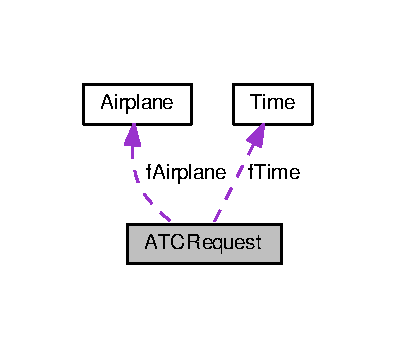
\includegraphics[width=190pt]{structATCRequest__coll__graph}
\end{center}
\end{figure}
\subsection*{Public Member Functions}
\begin{DoxyCompactItemize}
\item 
\hyperlink{structATCRequest_a26bd53c68bee460010bf80dc3c6dec12}{A\+T\+C\+Request} (\hyperlink{classTime}{Time} time, \hyperlink{classAirplane}{Airplane} $\ast$plane)
\end{DoxyCompactItemize}
\subsection*{Public Attributes}
\begin{DoxyCompactItemize}
\item 
\hyperlink{classTime}{Time} \hyperlink{structATCRequest_a6ef577c542082570fc934078994d622f}{f\+Time}
\item 
\hyperlink{classAirplane}{Airplane} $\ast$ \hyperlink{structATCRequest_a681215e14c24388ae811f182c33e4403}{f\+Airplane}
\end{DoxyCompactItemize}


\subsection{Constructor \& Destructor Documentation}
\index{A\+T\+C\+Request@{A\+T\+C\+Request}!A\+T\+C\+Request@{A\+T\+C\+Request}}
\index{A\+T\+C\+Request@{A\+T\+C\+Request}!A\+T\+C\+Request@{A\+T\+C\+Request}}
\subsubsection[{\texorpdfstring{A\+T\+C\+Request(\+Time time, Airplane $\ast$plane)}{ATCRequest(Time time, Airplane *plane)}}]{\setlength{\rightskip}{0pt plus 5cm}A\+T\+C\+Request\+::\+A\+T\+C\+Request (
\begin{DoxyParamCaption}
\item[{{\bf Time}}]{time, }
\item[{{\bf Airplane} $\ast$}]{plane}
\end{DoxyParamCaption}
)}\hypertarget{structATCRequest_a26bd53c68bee460010bf80dc3c6dec12}{}\label{structATCRequest_a26bd53c68bee460010bf80dc3c6dec12}
Constructor. 

\subsection{Member Data Documentation}
\index{A\+T\+C\+Request@{A\+T\+C\+Request}!f\+Airplane@{f\+Airplane}}
\index{f\+Airplane@{f\+Airplane}!A\+T\+C\+Request@{A\+T\+C\+Request}}
\subsubsection[{\texorpdfstring{f\+Airplane}{fAirplane}}]{\setlength{\rightskip}{0pt plus 5cm}{\bf Airplane}$\ast$ A\+T\+C\+Request\+::f\+Airplane}\hypertarget{structATCRequest_a681215e14c24388ae811f182c33e4403}{}\label{structATCRequest_a681215e14c24388ae811f182c33e4403}
\hyperlink{classAirplane}{Airplane} that sent request \index{A\+T\+C\+Request@{A\+T\+C\+Request}!f\+Time@{f\+Time}}
\index{f\+Time@{f\+Time}!A\+T\+C\+Request@{A\+T\+C\+Request}}
\subsubsection[{\texorpdfstring{f\+Time}{fTime}}]{\setlength{\rightskip}{0pt plus 5cm}{\bf Time} A\+T\+C\+Request\+::f\+Time}\hypertarget{structATCRequest_a6ef577c542082570fc934078994d622f}{}\label{structATCRequest_a6ef577c542082570fc934078994d622f}
\hyperlink{classTime}{Time} message was sent. 

The documentation for this struct was generated from the following files\+:\begin{DoxyCompactItemize}
\item 
/home/max/\+C\+Lion\+Projects/\+Project\+Vliegveld/headers/A\+T\+C.\+h\item 
/home/max/\+C\+Lion\+Projects/\+Project\+Vliegveld/src/A\+T\+C.\+cpp\end{DoxyCompactItemize}

\hypertarget{structComparator}{}\section{Comparator Struct Reference}
\label{structComparator}\index{Comparator@{Comparator}}
\subsection*{Public Member Functions}
\begin{DoxyCompactItemize}
\item 
bool {\bfseries operator()} (const \hyperlink{structATCRequest}{A\+T\+C\+Request} $\ast$lhs, const \hyperlink{structATCRequest}{A\+T\+C\+Request} $\ast$rhs)\hypertarget{structComparator_a9c98d44444d191fe54f5f3a5838600b5}{}\label{structComparator_a9c98d44444d191fe54f5f3a5838600b5}

\end{DoxyCompactItemize}


The documentation for this struct was generated from the following files\+:\begin{DoxyCompactItemize}
\item 
/home/max/\+C\+Lion\+Projects/\+Project\+Vliegveld/headers/A\+T\+C.\+h\item 
/home/max/\+C\+Lion\+Projects/\+Project\+Vliegveld/src/A\+T\+C.\+cpp\end{DoxyCompactItemize}

\hypertarget{classFlightPlan}{}\section{Flight\+Plan Class Reference}
\label{classFlightPlan}\index{Flight\+Plan@{Flight\+Plan}}


\+: Class that represents a flight plan in the simulation  




{\ttfamily \#include $<$Flight\+Plan.\+h$>$}

\subsection*{Public Member Functions}
\begin{DoxyCompactItemize}
\item 
\hyperlink{classFlightPlan_acc9140958ec2b86f78089067833f68fb}{Flight\+Plan} ()
\item 
\hyperlink{classFlightPlan_a674104757ac93924187fe1fc6bd7a342}{$\sim$\+Flight\+Plan} ()
\item 
bool \hyperlink{classFlightPlan_a6ba1f8f9cd4a738a437a3ec7ae283978}{properly\+Initialized} () const 
\item 
void \hyperlink{classFlightPlan_a54774b1bb6606e7b11359f23c2e4d79f}{set\+Departure} (int departure)
\item 
void \hyperlink{classFlightPlan_a1fad15b79c3463a21e8a89e6c42fda57}{set\+Arrival} (int arrival)
\item 
void \hyperlink{classFlightPlan_a157e8a456b078a125b64e20d6cd8bf58}{set\+Interval} (int interval)
\item 
E\+Event \hyperlink{classFlightPlan_a2350e5250fcc621240768e5dd7a7bdeb}{get\+Event} (\hyperlink{classTime}{Time} time)
\item 
bool \hyperlink{classFlightPlan_a28cda60a1a425003eb869a03b9f2b550}{complete} () const 
\item 
const std\+::string \& \hyperlink{classFlightPlan_add7c304a2be8ff8b6d08b6de28c1a4c6}{get\+Destination} () const 
\item 
void {\bfseries set\+Destination} (const std\+::string \&f\+Destination)\hypertarget{classFlightPlan_ab362a8718bf636c4c2e1738327879bed}{}\label{classFlightPlan_ab362a8718bf636c4c2e1738327879bed}

\item 
int {\bfseries get\+Departure} () const \hypertarget{classFlightPlan_a80708983bd926613c36041cf948c1224}{}\label{classFlightPlan_a80708983bd926613c36041cf948c1224}

\item 
int {\bfseries get\+Arrival} () const \hypertarget{classFlightPlan_a2f97aeefbe8a18e6e2f69fca5b3b9998}{}\label{classFlightPlan_a2f97aeefbe8a18e6e2f69fca5b3b9998}

\item 
int {\bfseries get\+Interval} () const \hypertarget{classFlightPlan_a9c15b66aa6fd54166a952e2d2c11cba3}{}\label{classFlightPlan_a9c15b66aa6fd54166a952e2d2c11cba3}

\item 
void {\bfseries set\+Airplane} (\hyperlink{classAirplane}{Airplane} $\ast$)\hypertarget{classFlightPlan_a9eb1f6f7f83913c1ff321095624cc11b}{}\label{classFlightPlan_a9eb1f6f7f83913c1ff321095624cc11b}

\item 
\hyperlink{classAirplane}{Airplane} $\ast$ {\bfseries get\+Airplane} () const \hypertarget{classFlightPlan_a6a65c9c90452c47e736eb0db04c69f38}{}\label{classFlightPlan_a6a65c9c90452c47e736eb0db04c69f38}

\end{DoxyCompactItemize}


\subsection{Detailed Description}
\+: Class that represents a flight plan in the simulation 

\subsection{Constructor \& Destructor Documentation}
\index{Flight\+Plan@{Flight\+Plan}!Flight\+Plan@{Flight\+Plan}}
\index{Flight\+Plan@{Flight\+Plan}!Flight\+Plan@{Flight\+Plan}}
\subsubsection[{\texorpdfstring{Flight\+Plan()}{FlightPlan()}}]{\setlength{\rightskip}{0pt plus 5cm}Flight\+Plan\+::\+Flight\+Plan (
\begin{DoxyParamCaption}
{}
\end{DoxyParamCaption}
)}\hypertarget{classFlightPlan_acc9140958ec2b86f78089067833f68fb}{}\label{classFlightPlan_acc9140958ec2b86f78089067833f68fb}
Default constructor ~\newline
 E\+N\+S\+U\+RE(\hyperlink{classFlightPlan_a6ba1f8f9cd4a738a437a3ec7ae283978}{properly\+Initialized()}, \char`\"{}constructor must end in properly\+Initialized state\char`\"{}); \index{Flight\+Plan@{Flight\+Plan}!````~Flight\+Plan@{$\sim$\+Flight\+Plan}}
\index{````~Flight\+Plan@{$\sim$\+Flight\+Plan}!Flight\+Plan@{Flight\+Plan}}
\subsubsection[{\texorpdfstring{$\sim$\+Flight\+Plan()}{~FlightPlan()}}]{\setlength{\rightskip}{0pt plus 5cm}Flight\+Plan\+::$\sim$\+Flight\+Plan (
\begin{DoxyParamCaption}
{}
\end{DoxyParamCaption}
)}\hypertarget{classFlightPlan_a674104757ac93924187fe1fc6bd7a342}{}\label{classFlightPlan_a674104757ac93924187fe1fc6bd7a342}
Destructor 

\subsection{Member Function Documentation}
\index{Flight\+Plan@{Flight\+Plan}!complete@{complete}}
\index{complete@{complete}!Flight\+Plan@{Flight\+Plan}}
\subsubsection[{\texorpdfstring{complete() const }{complete() const }}]{\setlength{\rightskip}{0pt plus 5cm}bool Flight\+Plan\+::complete (
\begin{DoxyParamCaption}
{}
\end{DoxyParamCaption}
) const}\hypertarget{classFlightPlan_a28cda60a1a425003eb869a03b9f2b550}{}\label{classFlightPlan_a28cda60a1a425003eb869a03b9f2b550}
Checks if all the data members were initialized ~\newline
 R\+E\+Q\+U\+I\+RE(this-\/$>$\hyperlink{classFlightPlan_a6ba1f8f9cd4a738a437a3ec7ae283978}{properly\+Initialized()}, \char`\"{}\+Flightplan was\textquotesingle{}t initialized when calling complete\char`\"{}); \begin{DoxyReturn}{Returns}
\+: boolean indicating if all members are initialized. 
\end{DoxyReturn}
\index{Flight\+Plan@{Flight\+Plan}!get\+Destination@{get\+Destination}}
\index{get\+Destination@{get\+Destination}!Flight\+Plan@{Flight\+Plan}}
\subsubsection[{\texorpdfstring{get\+Destination() const }{getDestination() const }}]{\setlength{\rightskip}{0pt plus 5cm}const string \& Flight\+Plan\+::get\+Destination (
\begin{DoxyParamCaption}
{}
\end{DoxyParamCaption}
) const}\hypertarget{classFlightPlan_add7c304a2be8ff8b6d08b6de28c1a4c6}{}\label{classFlightPlan_add7c304a2be8ff8b6d08b6de28c1a4c6}
Getters and setters for the fields of the class. For all\+: R\+E\+Q\+U\+I\+RE(\hyperlink{classFlightPlan_a6ba1f8f9cd4a738a437a3ec7ae283978}{properly\+Initialized()}, \char`\"{}\+Flightplan wasn\textquotesingle{}t properly initialized when calling getter/setter.\char`\"{}); \index{Flight\+Plan@{Flight\+Plan}!get\+Event@{get\+Event}}
\index{get\+Event@{get\+Event}!Flight\+Plan@{Flight\+Plan}}
\subsubsection[{\texorpdfstring{get\+Event(\+Time time)}{getEvent(Time time)}}]{\setlength{\rightskip}{0pt plus 5cm}E\+Event Flight\+Plan\+::get\+Event (
\begin{DoxyParamCaption}
\item[{{\bf Time}}]{time}
\end{DoxyParamCaption}
)}\hypertarget{classFlightPlan_a2350e5250fcc621240768e5dd7a7bdeb}{}\label{classFlightPlan_a2350e5250fcc621240768e5dd7a7bdeb}
Returns the event at the given time ~\newline
 R\+E\+Q\+U\+I\+RE(this-\/$>$\hyperlink{classFlightPlan_a6ba1f8f9cd4a738a437a3ec7ae283978}{properly\+Initialized()}, \char`\"{}\+Flightplan was\textquotesingle{}t initialized when calling get\+Event\char`\"{}); 
\begin{DoxyParams}{Parameters}
{\em time} & time to get event at \\
\hline
\end{DoxyParams}
\begin{DoxyReturn}{Returns}
event at this time 
\end{DoxyReturn}
\index{Flight\+Plan@{Flight\+Plan}!properly\+Initialized@{properly\+Initialized}}
\index{properly\+Initialized@{properly\+Initialized}!Flight\+Plan@{Flight\+Plan}}
\subsubsection[{\texorpdfstring{properly\+Initialized() const }{properlyInitialized() const }}]{\setlength{\rightskip}{0pt plus 5cm}bool Flight\+Plan\+::properly\+Initialized (
\begin{DoxyParamCaption}
{}
\end{DoxyParamCaption}
) const}\hypertarget{classFlightPlan_a6ba1f8f9cd4a738a437a3ec7ae283978}{}\label{classFlightPlan_a6ba1f8f9cd4a738a437a3ec7ae283978}
Checks if the object is properly initialized \begin{DoxyReturn}{Returns}
\+: boolean indicating if properly initialized 
\end{DoxyReturn}
\index{Flight\+Plan@{Flight\+Plan}!set\+Arrival@{set\+Arrival}}
\index{set\+Arrival@{set\+Arrival}!Flight\+Plan@{Flight\+Plan}}
\subsubsection[{\texorpdfstring{set\+Arrival(int arrival)}{setArrival(int arrival)}}]{\setlength{\rightskip}{0pt plus 5cm}void Flight\+Plan\+::set\+Arrival (
\begin{DoxyParamCaption}
\item[{int}]{arrival}
\end{DoxyParamCaption}
)}\hypertarget{classFlightPlan_a1fad15b79c3463a21e8a89e6c42fda57}{}\label{classFlightPlan_a1fad15b79c3463a21e8a89e6c42fda57}
Setter for arrival time ~\newline
 R\+E\+Q\+U\+I\+RE(this-\/$>$\hyperlink{classFlightPlan_a6ba1f8f9cd4a738a437a3ec7ae283978}{properly\+Initialized()}, \char`\"{}\+Flightplan was\textquotesingle{}t initialized when calling set\+Arrival\char`\"{}); ~\newline
 R\+E\+Q\+U\+I\+RE(arrival $>$= 0 \&\& arrival $<$ 60, \char`\"{}\+Arrival has to be between 0 and 60\char`\"{}); 
\begin{DoxyParams}{Parameters}
{\em arrival} & arrival time to set \\
\hline
\end{DoxyParams}
\index{Flight\+Plan@{Flight\+Plan}!set\+Departure@{set\+Departure}}
\index{set\+Departure@{set\+Departure}!Flight\+Plan@{Flight\+Plan}}
\subsubsection[{\texorpdfstring{set\+Departure(int departure)}{setDeparture(int departure)}}]{\setlength{\rightskip}{0pt plus 5cm}void Flight\+Plan\+::set\+Departure (
\begin{DoxyParamCaption}
\item[{int}]{departure}
\end{DoxyParamCaption}
)}\hypertarget{classFlightPlan_a54774b1bb6606e7b11359f23c2e4d79f}{}\label{classFlightPlan_a54774b1bb6606e7b11359f23c2e4d79f}
Setter for departure time ~\newline
 R\+E\+Q\+U\+I\+RE(this-\/$>$\hyperlink{classFlightPlan_a6ba1f8f9cd4a738a437a3ec7ae283978}{properly\+Initialized()}, \char`\"{}\+Flightplan was\textquotesingle{}t initialized when calling set\+Departure\char`\"{}); ~\newline
 R\+E\+Q\+U\+I\+RE(departure $>$= 0 \&\& departure $<$ 60, \char`\"{}\+Departure has to be between 0 and 60\char`\"{}); 
\begin{DoxyParams}{Parameters}
{\em departure} & departure time to set \\
\hline
\end{DoxyParams}
\index{Flight\+Plan@{Flight\+Plan}!set\+Interval@{set\+Interval}}
\index{set\+Interval@{set\+Interval}!Flight\+Plan@{Flight\+Plan}}
\subsubsection[{\texorpdfstring{set\+Interval(int interval)}{setInterval(int interval)}}]{\setlength{\rightskip}{0pt plus 5cm}void Flight\+Plan\+::set\+Interval (
\begin{DoxyParamCaption}
\item[{int}]{interval}
\end{DoxyParamCaption}
)}\hypertarget{classFlightPlan_a157e8a456b078a125b64e20d6cd8bf58}{}\label{classFlightPlan_a157e8a456b078a125b64e20d6cd8bf58}
Setter for interval ~\newline
 R\+E\+Q\+U\+I\+RE(this-\/$>$\hyperlink{classFlightPlan_a6ba1f8f9cd4a738a437a3ec7ae283978}{properly\+Initialized()}, \char`\"{}\+Flightplan was\textquotesingle{}t initialized when calling set\+Interval\char`\"{}); ~\newline
 R\+E\+Q\+U\+I\+RE(interval $>$ 0, \char`\"{}\+Interval has to be at least 1\char`\"{}); 
\begin{DoxyParams}{Parameters}
{\em interval} & interval to set \\
\hline
\end{DoxyParams}


The documentation for this class was generated from the following files\+:\begin{DoxyCompactItemize}
\item 
/home/max/\+C\+Lion\+Projects/\+Project\+Vliegveld/headers/Flight\+Plan.\+h\item 
/home/max/\+C\+Lion\+Projects/\+Project\+Vliegveld/src/Flight\+Plan.\+cpp\end{DoxyCompactItemize}

\hypertarget{classGraphics}{}\section{Graphics Class Reference}
\label{classGraphics}\index{Graphics@{Graphics}}


{\ttfamily \#include $<$Graphics.\+h$>$}

\subsection*{Public Member Functions}
\begin{DoxyCompactItemize}
\item 
\hyperlink{classGraphics_aeb4dc61589dbc318e3b9b91da1079a73}{Graphics} (\hyperlink{classAirport}{Airport} $\ast$airport)
\item 
void \hyperlink{classGraphics_a0fe625122d443cffbc405e9f49808cd7}{add\+Element} (\hyperlink{classAirplane}{Airplane} $\ast$airplane)
\item 
void \hyperlink{classGraphics_a3dca71401d21a07a2c0a9d1f44df0d3c}{add\+Element} (\hyperlink{classRunway}{Runway} $\ast$runway)
\item 
std\+::string \hyperlink{classGraphics_a7650057214dabce915dfc6f104e0b1eb}{generate\+I\+NI} (double x, double y, double z, int size=3000) const 
\item 
bool \hyperlink{classGraphics_ac10231e8c943b3218a0d0260abf2065f}{properly\+Initialized} () const 
\end{DoxyCompactItemize}


\subsection{Detailed Description}
Class that generates a string in valid .ini format. ~\newline
 This string can be used with the \hyperlink{classGraphics}{Graphics} Engine to generate an image ~\newline
 of all the added elements and thus the airport. 

\subsection{Constructor \& Destructor Documentation}
\index{Graphics@{Graphics}!Graphics@{Graphics}}
\index{Graphics@{Graphics}!Graphics@{Graphics}}
\subsubsection[{\texorpdfstring{Graphics(\+Airport $\ast$airport)}{Graphics(Airport *airport)}}]{\setlength{\rightskip}{0pt plus 5cm}Graphics\+::\+Graphics (
\begin{DoxyParamCaption}
\item[{{\bf Airport} $\ast$}]{airport}
\end{DoxyParamCaption}
)}\hypertarget{classGraphics_aeb4dc61589dbc318e3b9b91da1079a73}{}\label{classGraphics_aeb4dc61589dbc318e3b9b91da1079a73}
Constructor. Adds the figures for the gates. ~\newline
 E\+N\+S\+U\+RE(\hyperlink{classGraphics_ac10231e8c943b3218a0d0260abf2065f}{properly\+Initialized()}, \char`\"{}\+Graphics object was not properly constructed\char`\"{}); 
\begin{DoxyParams}{Parameters}
{\em airport} & airport in the simulation \\
\hline
\end{DoxyParams}


\subsection{Member Function Documentation}
\index{Graphics@{Graphics}!add\+Element@{add\+Element}}
\index{add\+Element@{add\+Element}!Graphics@{Graphics}}
\subsubsection[{\texorpdfstring{add\+Element(\+Airplane $\ast$airplane)}{addElement(Airplane *airplane)}}]{\setlength{\rightskip}{0pt plus 5cm}void Graphics\+::add\+Element (
\begin{DoxyParamCaption}
\item[{{\bf Airplane} $\ast$}]{airplane}
\end{DoxyParamCaption}
)}\hypertarget{classGraphics_a0fe625122d443cffbc405e9f49808cd7}{}\label{classGraphics_a0fe625122d443cffbc405e9f49808cd7}
Adds the figures for an airplane. ~\newline
 The position is calculated with the status and position of the airplane. ~\newline
 R\+E\+Q\+U\+I\+RE(\hyperlink{classGraphics_ac10231e8c943b3218a0d0260abf2065f}{properly\+Initialized()}, \char`\"{}\+Graphics was not properly initialized when calling add\+Element(airplane)\char`\"{}); ~\newline
 R\+E\+Q\+U\+I\+RE(runway != N\+U\+LL, \char`\"{}\+Element can\textquotesingle{}t be N\+U\+L\+L when calling add\+Element\char`\"{}); 
\begin{DoxyParams}{Parameters}
{\em airplane} & the airplane to be added \\
\hline
\end{DoxyParams}
\index{Graphics@{Graphics}!add\+Element@{add\+Element}}
\index{add\+Element@{add\+Element}!Graphics@{Graphics}}
\subsubsection[{\texorpdfstring{add\+Element(\+Runway $\ast$runway)}{addElement(Runway *runway)}}]{\setlength{\rightskip}{0pt plus 5cm}void Graphics\+::add\+Element (
\begin{DoxyParamCaption}
\item[{{\bf Runway} $\ast$}]{runway}
\end{DoxyParamCaption}
)}\hypertarget{classGraphics_a3dca71401d21a07a2c0a9d1f44df0d3c}{}\label{classGraphics_a3dca71401d21a07a2c0a9d1f44df0d3c}
Adds the figures for a runway. ~\newline
 The position is calculated by the number of runways already added ~\newline
 R\+E\+Q\+U\+I\+RE(\hyperlink{classGraphics_ac10231e8c943b3218a0d0260abf2065f}{properly\+Initialized()}, \char`\"{}\+Graphics was not properly initialized when calling add\+Element(runway)\char`\"{}); ~\newline
 R\+E\+Q\+U\+I\+RE(airplane != N\+U\+LL, \char`\"{}\+Element can\textquotesingle{}t be N\+U\+L\+L when calling add\+Element\char`\"{}); 
\begin{DoxyParams}{Parameters}
{\em runway} & the runway to be added \\
\hline
\end{DoxyParams}
\index{Graphics@{Graphics}!generate\+I\+NI@{generate\+I\+NI}}
\index{generate\+I\+NI@{generate\+I\+NI}!Graphics@{Graphics}}
\subsubsection[{\texorpdfstring{generate\+I\+N\+I(double x, double y, double z, int size=3000) const }{generateINI(double x, double y, double z, int size=3000) const }}]{\setlength{\rightskip}{0pt plus 5cm}std\+::string Graphics\+::generate\+I\+NI (
\begin{DoxyParamCaption}
\item[{double}]{x, }
\item[{double}]{y, }
\item[{double}]{z, }
\item[{int}]{size = {\ttfamily 3000}}
\end{DoxyParamCaption}
) const}\hypertarget{classGraphics_a7650057214dabce915dfc6f104e0b1eb}{}\label{classGraphics_a7650057214dabce915dfc6f104e0b1eb}
Generates the ini file of all the elements in the figures vector. ~\newline
 R\+E\+Q\+U\+I\+RE(\hyperlink{classGraphics_ac10231e8c943b3218a0d0260abf2065f}{properly\+Initialized()}, \char`\"{}\+Graphics was not properly initialized when calling generate\+I\+N\+I\char`\"{}); ~\newline
 R\+E\+Q\+U\+I\+RE(size $>$ 0, \char`\"{}\+Size can\textquotesingle{}t be negative\char`\"{}); 
\begin{DoxyParams}{Parameters}
{\em x} & eye point x coordinate \\
\hline
{\em y} & eye point y coordinate \\
\hline
{\em z} & eye point z coordinate \\
\hline
\end{DoxyParams}
\begin{DoxyReturn}{Returns}
string in valid ini format 
\end{DoxyReturn}
\index{Graphics@{Graphics}!properly\+Initialized@{properly\+Initialized}}
\index{properly\+Initialized@{properly\+Initialized}!Graphics@{Graphics}}
\subsubsection[{\texorpdfstring{properly\+Initialized() const }{properlyInitialized() const }}]{\setlength{\rightskip}{0pt plus 5cm}bool Graphics\+::properly\+Initialized (
\begin{DoxyParamCaption}
{}
\end{DoxyParamCaption}
) const}\hypertarget{classGraphics_ac10231e8c943b3218a0d0260abf2065f}{}\label{classGraphics_ac10231e8c943b3218a0d0260abf2065f}
Checks if the object is properly initialized \begin{DoxyReturn}{Returns}
\+: Boolean indicating if properly initialized or not. 
\end{DoxyReturn}


The documentation for this class was generated from the following files\+:\begin{DoxyCompactItemize}
\item 
/home/max/\+C\+Lion\+Projects/\+Project\+Vliegveld/headers/Graphics.\+h\item 
/home/max/\+C\+Lion\+Projects/\+Project\+Vliegveld/src/Graphics.\+cpp\end{DoxyCompactItemize}

\hypertarget{classInput}{}\section{Input Class Reference}
\label{classInput}\index{Input@{Input}}


\+: Class that reads input for the simulation  




{\ttfamily \#include $<$Input.\+h$>$}

\subsection*{Public Member Functions}
\begin{DoxyCompactItemize}
\item 
\hyperlink{classInput_abae3f379d3f157cf42dc857309832dba}{Input} ()
\item 
bool \hyperlink{classInput_a42a0d1fd763cb2814cefe27b144ae0bb}{properly\+Initialized} () const 
\item 
void \hyperlink{classInput_abb78078475f91c654db63c392aefbf51}{read} (const string \&filename, ostream \&error\+Log=cerr)
\item 
void \hyperlink{classInput_adf2ec48d79d704c139f9a2ab295f8d21}{add\+Airport} (\hyperlink{classAirport}{Airport} $\ast$airport)
\item 
void \hyperlink{classInput_a047b280ecbd65bf8be570aba4f07f440}{add\+Runway} (\hyperlink{classRunway}{Runway} $\ast$runway)
\item 
void \hyperlink{classInput_af6a650235d15f760ec8764645ce19bc9}{add\+Flightplan} (\hyperlink{classFlightplan}{Flightplan} $\ast$flightplan)
\item 
\hyperlink{classAirport}{Airport} $\ast$ \hyperlink{classInput_a554acd227613a3b7ac86bce4d41060c7}{find\+Airport\+By\+I\+A\+TA} (const string \&iata) const 
\item 
vector$<$ \hyperlink{classAirport}{Airport} $\ast$ $>$ \hyperlink{classInput_aa1f634b15684092240be80cb17dd28ec}{get\+Airports} () const 
\item 
vector$<$ \hyperlink{classFlightplan}{Flightplan} $\ast$ $>$ \hyperlink{classInput_af03591fafa66902f7f4050b37e6b428e}{get\+Flightplans} () const 
\end{DoxyCompactItemize}
\subsection*{Static Public Member Functions}
\begin{DoxyCompactItemize}
\item 
static bool \hyperlink{classInput_a07fca98c3279dbcb8d49afa59bd9ad7f}{is\+Number} (const string \&)
\end{DoxyCompactItemize}


\subsection{Detailed Description}
\+: Class that reads input for the simulation 

\subsection{Constructor \& Destructor Documentation}
\index{Input@{Input}!Input@{Input}}
\index{Input@{Input}!Input@{Input}}
\subsubsection[{\texorpdfstring{Input()}{Input()}}]{\setlength{\rightskip}{0pt plus 5cm}Input\+::\+Input (
\begin{DoxyParamCaption}
{}
\end{DoxyParamCaption}
)}\hypertarget{classInput_abae3f379d3f157cf42dc857309832dba}{}\label{classInput_abae3f379d3f157cf42dc857309832dba}
Default constructor ~\newline
 E\+N\+S\+U\+RE(\hyperlink{classInput_a42a0d1fd763cb2814cefe27b144ae0bb}{properly\+Initialized()}, \char`\"{}constructor must end in properly\+Initialized state\char`\"{}); 
\begin{DoxyCode}
47              \{
48     fInitCheck = \textcolor{keyword}{this};
49     \hyperlink{DesignByContract_8h_ab8da60ea2bcdd55183cc29d8526e6857}{ENSURE}(\hyperlink{classInput_a42a0d1fd763cb2814cefe27b144ae0bb}{properlyInitialized}(), \textcolor{stringliteral}{"constructor must end in properlyInitialized
       state"});
50 \}
\end{DoxyCode}


\subsection{Member Function Documentation}
\index{Input@{Input}!add\+Airport@{add\+Airport}}
\index{add\+Airport@{add\+Airport}!Input@{Input}}
\subsubsection[{\texorpdfstring{add\+Airport(\+Airport $\ast$airport)}{addAirport(Airport *airport)}}]{\setlength{\rightskip}{0pt plus 5cm}void Input\+::add\+Airport (
\begin{DoxyParamCaption}
\item[{{\bf Airport} $\ast$}]{airport}
\end{DoxyParamCaption}
)}\hypertarget{classInput_adf2ec48d79d704c139f9a2ab295f8d21}{}\label{classInput_adf2ec48d79d704c139f9a2ab295f8d21}
Adds an airport to the simulation ~\newline
 R\+E\+Q\+U\+I\+RE(this-\/$>$\hyperlink{classInput_a42a0d1fd763cb2814cefe27b144ae0bb}{properly\+Initialized()}, \char`\"{}\+Input was\textquotesingle{}t initialized when calling add\+Airport\char`\"{}); ~\newline
 R\+E\+Q\+U\+I\+RE(airport-\/$>$complete(), \char`\"{}\+Airport has to be completely initialized to add it to the simulation\char`\"{}); ~\newline
 E\+N\+S\+U\+RE(airports.\+back() == airport, \char`\"{}\+Airplane was not added to simulation.\char`\"{}); 
\begin{DoxyCode}
517                                        \{
518     \hyperlink{DesignByContract_8h_aeb774672b46dbe80afc14e0d1970f017}{REQUIRE}(this->\hyperlink{classInput_a42a0d1fd763cb2814cefe27b144ae0bb}{properlyInitialized}(), \textcolor{stringliteral}{"Input was't initialized when calling
       addAirport"});
519     \hyperlink{DesignByContract_8h_aeb774672b46dbe80afc14e0d1970f017}{REQUIRE}(airport->\hyperlink{classAirport_a76819017f88f563183bd16a0b4da4e40}{complete}(), \textcolor{stringliteral}{"Airport has to be completely initialized to add it to the
       simulation"});
520     \textcolor{comment}{// Initialize gateStack}
521     airport->\hyperlink{classAirport_a2a4915cb5db8ff9a992c262af3f333cb}{initStack}();
522 
523     \textcolor{comment}{// Add to vec}
524     airports.push\_back(airport);
525 
526     \hyperlink{DesignByContract_8h_ab8da60ea2bcdd55183cc29d8526e6857}{ENSURE}(airports.back() == airport, \textcolor{stringliteral}{"Airplane was not added to simulation."});
527 \}
\end{DoxyCode}
\index{Input@{Input}!add\+Flightplan@{add\+Flightplan}}
\index{add\+Flightplan@{add\+Flightplan}!Input@{Input}}
\subsubsection[{\texorpdfstring{add\+Flightplan(\+Flightplan $\ast$flightplan)}{addFlightplan(Flightplan *flightplan)}}]{\setlength{\rightskip}{0pt plus 5cm}void Input\+::add\+Flightplan (
\begin{DoxyParamCaption}
\item[{{\bf Flightplan} $\ast$}]{flightplan}
\end{DoxyParamCaption}
)}\hypertarget{classInput_af6a650235d15f760ec8764645ce19bc9}{}\label{classInput_af6a650235d15f760ec8764645ce19bc9}
Adds a flightplan to the simulation with the given specifications ~\newline
 R\+E\+Q\+U\+I\+RE(this-\/$>$\hyperlink{classInput_a42a0d1fd763cb2814cefe27b144ae0bb}{properly\+Initialized()}, \char`\"{}\+Input was\textquotesingle{}t initialized when calling add\+Flightplan\char`\"{}); ~\newline
 R\+E\+Q\+U\+I\+RE(flightplan-\/$>$complete(), \char`\"{}\+Flightplan has to be completely initialized to add it to the simulation\char`\"{}); ~\newline
 E\+N\+S\+U\+RE(flightplans.\+back() == flightplan, \char`\"{}\+Flightplan was not added to simulation.\char`\"{}); 
\begin{DoxyCode}
536                                                 \{
537     \hyperlink{DesignByContract_8h_aeb774672b46dbe80afc14e0d1970f017}{REQUIRE}(this->\hyperlink{classInput_a42a0d1fd763cb2814cefe27b144ae0bb}{properlyInitialized}(), \textcolor{stringliteral}{"Input was't initialized when calling
       addFlightplan"});
538     \hyperlink{DesignByContract_8h_aeb774672b46dbe80afc14e0d1970f017}{REQUIRE}(flightplan->\hyperlink{classFlightplan_a07f564cb5e5cdbad4abb2098f7941597}{complete}(), \textcolor{stringliteral}{"Flightplan has to be completely initialized to add it
       to the simulation"});
539     flightplans.push\_back(flightplan);
540     \hyperlink{DesignByContract_8h_ab8da60ea2bcdd55183cc29d8526e6857}{ENSURE}(flightplans.back() == flightplan, \textcolor{stringliteral}{"Flightplan was not added to simulation."});
541 \}
\end{DoxyCode}
\index{Input@{Input}!add\+Runway@{add\+Runway}}
\index{add\+Runway@{add\+Runway}!Input@{Input}}
\subsubsection[{\texorpdfstring{add\+Runway(\+Runway $\ast$runway)}{addRunway(Runway *runway)}}]{\setlength{\rightskip}{0pt plus 5cm}void Input\+::add\+Runway (
\begin{DoxyParamCaption}
\item[{{\bf Runway} $\ast$}]{runway}
\end{DoxyParamCaption}
)}\hypertarget{classInput_a047b280ecbd65bf8be570aba4f07f440}{}\label{classInput_a047b280ecbd65bf8be570aba4f07f440}
Adds a runway to the simulation with the given specifications ~\newline
 R\+E\+Q\+U\+I\+RE(this-\/$>$\hyperlink{classInput_a42a0d1fd763cb2814cefe27b144ae0bb}{properly\+Initialized()}, \char`\"{}\+Input was\textquotesingle{}t initialized when calling add\+Runway\char`\"{}); ~\newline
 R\+E\+Q\+U\+I\+RE(runway-\/$>$complete(), \char`\"{}\+Runway has to be completely initialized to add it to the simulation\char`\"{}); ~\newline
 E\+N\+S\+U\+RE(runway-\/$>$get\+Airport()-\/$>$get\+Runways().back() == runway, \char`\"{}\+Runway was not added to the airport\char`\"{}); 
\begin{DoxyCode}
529                                     \{
530     \hyperlink{DesignByContract_8h_aeb774672b46dbe80afc14e0d1970f017}{REQUIRE}(this->\hyperlink{classInput_a42a0d1fd763cb2814cefe27b144ae0bb}{properlyInitialized}(), \textcolor{stringliteral}{"Input was't initialized when calling
       addRunway"});
531     \hyperlink{DesignByContract_8h_aeb774672b46dbe80afc14e0d1970f017}{REQUIRE}(runway->\hyperlink{classRunway_a3f905e251e1c7941690cf89c1fabd04c}{complete}(), \textcolor{stringliteral}{"Runway has to be completely initialized to add it to the
       simulation"});
532     runway->\hyperlink{classRunway_a8a16d41a8c65a85e433d96faafb5de06}{getAirport}()->\hyperlink{classAirport_a346e81f1bbb8b9eb9a0eee341d947fc1}{addRunway}(runway);
533     \hyperlink{DesignByContract_8h_ab8da60ea2bcdd55183cc29d8526e6857}{ENSURE}(runway->\hyperlink{classRunway_a8a16d41a8c65a85e433d96faafb5de06}{getAirport}()->\hyperlink{classAirport_a14310ffeba8a024105071c156fd42cf7}{getRunways}().back() == runway, \textcolor{stringliteral}{"Runway was not
       added to the airport"});
534 \}
\end{DoxyCode}
\index{Input@{Input}!find\+Airport\+By\+I\+A\+TA@{find\+Airport\+By\+I\+A\+TA}}
\index{find\+Airport\+By\+I\+A\+TA@{find\+Airport\+By\+I\+A\+TA}!Input@{Input}}
\subsubsection[{\texorpdfstring{find\+Airport\+By\+I\+A\+T\+A(const string \&iata) const }{findAirportByIATA(const string &iata) const }}]{\setlength{\rightskip}{0pt plus 5cm}{\bf Airport} $\ast$ Input\+::find\+Airport\+By\+I\+A\+TA (
\begin{DoxyParamCaption}
\item[{const string \&}]{iata}
\end{DoxyParamCaption}
) const}\hypertarget{classInput_a554acd227613a3b7ac86bce4d41060c7}{}\label{classInput_a554acd227613a3b7ac86bce4d41060c7}
Finds an airport with a specific I\+A\+TA ~\newline
 R\+E\+Q\+U\+I\+RE(this-\/$>$\hyperlink{classInput_a42a0d1fd763cb2814cefe27b144ae0bb}{properly\+Initialized()}, \char`\"{}\+Input was\textquotesingle{}t initialized when calling find\+Airport\+By\+I\+A\+T\+A\char`\"{}); 
\begin{DoxyCode}
543                                                           \{
544     \hyperlink{DesignByContract_8h_aeb774672b46dbe80afc14e0d1970f017}{REQUIRE}(this->\hyperlink{classInput_a42a0d1fd763cb2814cefe27b144ae0bb}{properlyInitialized}(), \textcolor{stringliteral}{"Input was't initialized when calling
       findAirportByIATA"});
545     \textcolor{comment}{// Check all Airports and if the Airport matches the IATA, return this Airport.}
546     vector<Airport*>::const\_iterator itr;
547     \textcolor{keywordflow}{for} (itr = airports.begin(); itr < airports.end(); ++itr) \{
548         \hyperlink{classAirport}{Airport}* cur\_ap = *itr;
549         \textcolor{keywordflow}{if} (cur\_ap->\hyperlink{classAirport_a4550198ddc92d3583a0f3c31278189b2}{getIata}() == iata) \{
550             \textcolor{keywordflow}{return} cur\_ap;
551         \}
552     \}
553     \textcolor{keywordflow}{return} NULL;
554 \}
\end{DoxyCode}
\index{Input@{Input}!get\+Airports@{get\+Airports}}
\index{get\+Airports@{get\+Airports}!Input@{Input}}
\subsubsection[{\texorpdfstring{get\+Airports() const }{getAirports() const }}]{\setlength{\rightskip}{0pt plus 5cm}vector$<$ {\bf Airport} $\ast$ $>$ Input\+::get\+Airports (
\begin{DoxyParamCaption}
{}
\end{DoxyParamCaption}
) const}\hypertarget{classInput_aa1f634b15684092240be80cb17dd28ec}{}\label{classInput_aa1f634b15684092240be80cb17dd28ec}
Getter for the airports in the simulation ~\newline
 R\+E\+Q\+U\+I\+RE(this-\/$>$\hyperlink{classInput_a42a0d1fd763cb2814cefe27b144ae0bb}{properly\+Initialized()}, \char`\"{}\+Input was\textquotesingle{}t initialized when calling get\+Airports\char`\"{}); \begin{DoxyReturn}{Returns}
vec of all airports 
\end{DoxyReturn}

\begin{DoxyCode}
556                                           \{
557     \hyperlink{DesignByContract_8h_aeb774672b46dbe80afc14e0d1970f017}{REQUIRE}(this->\hyperlink{classInput_a42a0d1fd763cb2814cefe27b144ae0bb}{properlyInitialized}(), \textcolor{stringliteral}{"Input was't initialized when calling
       getAirports"});
558     \textcolor{keywordflow}{return} Input::airports;
559 \}
\end{DoxyCode}
\index{Input@{Input}!get\+Flightplans@{get\+Flightplans}}
\index{get\+Flightplans@{get\+Flightplans}!Input@{Input}}
\subsubsection[{\texorpdfstring{get\+Flightplans() const }{getFlightplans() const }}]{\setlength{\rightskip}{0pt plus 5cm}vector$<$ {\bf Flightplan} $\ast$ $>$ Input\+::get\+Flightplans (
\begin{DoxyParamCaption}
{}
\end{DoxyParamCaption}
) const}\hypertarget{classInput_af03591fafa66902f7f4050b37e6b428e}{}\label{classInput_af03591fafa66902f7f4050b37e6b428e}
Getter for the flightplans in the simulation ~\newline
 R\+E\+Q\+U\+I\+RE(this-\/$>$\hyperlink{classInput_a42a0d1fd763cb2814cefe27b144ae0bb}{properly\+Initialized()}, \char`\"{}\+Input was\textquotesingle{}t initialized when calling get\+Flightplans\char`\"{}); \begin{DoxyReturn}{Returns}
vec of all flightplans 
\end{DoxyReturn}

\begin{DoxyCode}
561                                                 \{
562     \hyperlink{DesignByContract_8h_aeb774672b46dbe80afc14e0d1970f017}{REQUIRE}(this->\hyperlink{classInput_a42a0d1fd763cb2814cefe27b144ae0bb}{properlyInitialized}(), \textcolor{stringliteral}{"Input was't initialized when calling
       getFlightplans"});
563     \textcolor{keywordflow}{return} flightplans;
564 \}
\end{DoxyCode}
\index{Input@{Input}!is\+Number@{is\+Number}}
\index{is\+Number@{is\+Number}!Input@{Input}}
\subsubsection[{\texorpdfstring{is\+Number(const string \&)}{isNumber(const string &)}}]{\setlength{\rightskip}{0pt plus 5cm}bool Input\+::is\+Number (
\begin{DoxyParamCaption}
\item[{const string \&}]{input}
\end{DoxyParamCaption}
)\hspace{0.3cm}{\ttfamily [static]}}\hypertarget{classInput_a07fca98c3279dbcb8d49afa59bd9ad7f}{}\label{classInput_a07fca98c3279dbcb8d49afa59bd9ad7f}
Checks if a given string is a valid unsigned int ~\newline
 R\+E\+Q\+U\+I\+RE(this-\/$>$\hyperlink{classInput_a42a0d1fd763cb2814cefe27b144ae0bb}{properly\+Initialized()}, \char`\"{}\+Input was\textquotesingle{}t initialized when calling is\+Number\char`\"{}); 
\begin{DoxyCode}
570                                         \{
571     string::const\_iterator it;
572     \textcolor{keywordflow}{for} (it = input.begin(); it != input.end(); ++it) \{
573         \textcolor{keywordflow}{if} (!isdigit(*it)) \{
574             \textcolor{keywordflow}{return} \textcolor{keyword}{false};
575         \}
576     \}
577     \textcolor{keywordflow}{return} \textcolor{keyword}{true};
578 \}\end{DoxyCode}
\index{Input@{Input}!properly\+Initialized@{properly\+Initialized}}
\index{properly\+Initialized@{properly\+Initialized}!Input@{Input}}
\subsubsection[{\texorpdfstring{properly\+Initialized() const }{properlyInitialized() const }}]{\setlength{\rightskip}{0pt plus 5cm}bool Input\+::properly\+Initialized (
\begin{DoxyParamCaption}
{}
\end{DoxyParamCaption}
) const}\hypertarget{classInput_a42a0d1fd763cb2814cefe27b144ae0bb}{}\label{classInput_a42a0d1fd763cb2814cefe27b144ae0bb}
Checks if the object is properly initialized 
\begin{DoxyCode}
566                                       \{
567     \textcolor{keywordflow}{return} fInitCheck == \textcolor{keyword}{this};
568 \}
\end{DoxyCode}
\index{Input@{Input}!read@{read}}
\index{read@{read}!Input@{Input}}
\subsubsection[{\texorpdfstring{read(const string \&filename, ostream \&error\+Log=cerr)}{read(const string &filename, ostream &errorLog=cerr)}}]{\setlength{\rightskip}{0pt plus 5cm}void Input\+::read (
\begin{DoxyParamCaption}
\item[{const string \&}]{filename, }
\item[{ostream \&}]{error\+Log = {\ttfamily cerr}}
\end{DoxyParamCaption}
)}\hypertarget{classInput_abb78078475f91c654db63c392aefbf51}{}\label{classInput_abb78078475f91c654db63c392aefbf51}
Reads the given file and stores the information ~\newline
 R\+E\+Q\+U\+I\+RE(this-\/$>$\hyperlink{classInput_a42a0d1fd763cb2814cefe27b144ae0bb}{properly\+Initialized()}, \char`\"{}\+Input was\textquotesingle{}t initialized when calling read\char`\"{}); 
\begin{DoxyParams}{Parameters}
{\em filename} & name of the file with input \\
\hline
\end{DoxyParams}

\begin{DoxyCode}
9                                                           \{
10     \textcolor{comment}{// Load xml file, program will end if failed}
11     TiXmlDocument xml;
12     \textcolor{keywordtype}{string} error = \textcolor{stringliteral}{"Couldn't open "} + filename + \textcolor{stringliteral}{"."};
13     \textcolor{keywordflow}{if} (!xml.LoadFile(filename.c\_str())) \{
14         errorLog << xml.ErrorDesc() << endl;
15         xml.Clear();
16     \}
17     \hyperlink{DesignByContract_8h_aeb774672b46dbe80afc14e0d1970f017}{REQUIRE}(xml.LoadFile(filename.c\_str()), error.c\_str());
18 
19     \textcolor{comment}{// We iterate over all root elements.}
20     \textcolor{keywordflow}{for} (TiXmlElement *root = xml.FirstChildElement(); root != NULL; root = root->NextSiblingElement()) \{
21 
22         \textcolor{comment}{// Airports}
23         \textcolor{keywordflow}{if} (strcmp(root->Value(), \textcolor{stringliteral}{"AIRPORT"}) == 0) \{
24             readAirport(root->FirstChildElement(), errorLog);
25         \}
26 
27         \textcolor{comment}{// Runways}
28         \textcolor{keywordflow}{else} \textcolor{keywordflow}{if} (strcmp(root->Value(), \textcolor{stringliteral}{"RUNWAY"}) == 0) \{
29             readRunway(root->FirstChildElement(), errorLog);
30         \}
31 
32         \textcolor{comment}{// Airplanes}
33         \textcolor{keywordflow}{else} \textcolor{keywordflow}{if} (strcmp(root->Value(), \textcolor{stringliteral}{"AIRPLANE"}) == 0) \{
34             readAirplane(root->FirstChildElement(), errorLog);
35         \}
36 
37         \textcolor{comment}{// Invalid element}
38         \textcolor{keywordflow}{else} \{
39             errorLog << \textcolor{stringliteral}{"Did not recognize element: "} << root->Value() << endl;
40         \}
41     \}
42 
43     \textcolor{comment}{// We are finished with our XML file, so we clear it.}
44     xml.Clear();
45 \}
\end{DoxyCode}


The documentation for this class was generated from the following files\+:\begin{DoxyCompactItemize}
\item 
/home/max/\+C\+Lion\+Projects/\+Project\+Vliegveld/headers/\hyperlink{Input_8h}{Input.\+h}\item 
/home/max/\+C\+Lion\+Projects/\+Project\+Vliegveld/src/\hyperlink{Input_8cpp}{Input.\+cpp}\end{DoxyCompactItemize}

\hypertarget{classRunway}{}\section{Runway Class Reference}
\label{classRunway}\index{Runway@{Runway}}


{\ttfamily \#include $<$Runway.\+h$>$}

\subsection*{Public Member Functions}
\begin{DoxyCompactItemize}
\item 
\hyperlink{classRunway_a75b9355b4953bd430f7c6ea0a18b465a}{Runway} ()
\item 
bool \hyperlink{classRunway_a3f905e251e1c7941690cf89c1fabd04c}{complete} () const 
\item 
bool \hyperlink{classRunway_ab1eb6649c04ead1c6ba6405b0d6e2a9f}{properly\+Initialized} () const 
\item 
bool \hyperlink{classRunway_a54aa6c5f9054cc5d16c10257c641f997}{valid\+For\+Airplane} (\hyperlink{classAirplane}{Airplane} $\ast$plane) const 
\item 
E\+Runway\+Type \hyperlink{classRunway_a6d936a840916f8a5fe01551622cf6c46}{get\+Type} () const 
\item 
void {\bfseries set\+Type} (E\+Runway\+Type type)\hypertarget{classRunway_a0a95f11d67cb4677f1bddd8cf20ed5bc}{}\label{classRunway_a0a95f11d67cb4677f1bddd8cf20ed5bc}

\item 
int {\bfseries get\+Length} () const \hypertarget{classRunway_ab22377036fde6582fa86441e73ad69d2}{}\label{classRunway_ab22377036fde6582fa86441e73ad69d2}

\item 
void {\bfseries set\+Length} (int length)\hypertarget{classRunway_af32954dc4688acd3a91114d200c6df9e}{}\label{classRunway_af32954dc4688acd3a91114d200c6df9e}

\item 
const std\+::string \& {\bfseries get\+Name} () const \hypertarget{classRunway_a2934c38f3af6080f7b40c306a27c57cd}{}\label{classRunway_a2934c38f3af6080f7b40c306a27c57cd}

\item 
void {\bfseries set\+Name} (const std\+::string \&f\+Name)\hypertarget{classRunway_a7c2e26b48213f220676d24dc7e102f4c}{}\label{classRunway_a7c2e26b48213f220676d24dc7e102f4c}

\item 
bool {\bfseries is\+Free} () const \hypertarget{classRunway_a7696b8546ad5ba33d401d7ba740c5936}{}\label{classRunway_a7696b8546ad5ba33d401d7ba740c5936}

\item 
void {\bfseries set\+Free} (bool free)\hypertarget{classRunway_aa93f02e87a66d6ac6ff49ebaf6919216}{}\label{classRunway_aa93f02e87a66d6ac6ff49ebaf6919216}

\item 
std\+::string {\bfseries get\+Taxi\+Point} () const \hypertarget{classRunway_ad2d8fd5696ec93e2fa3d32bec3d02f59}{}\label{classRunway_ad2d8fd5696ec93e2fa3d32bec3d02f59}

\item 
void {\bfseries set\+Taxi\+Point} (const std\+::string \&)\hypertarget{classRunway_aef252fe353421b36fca0f0546eb258de}{}\label{classRunway_aef252fe353421b36fca0f0546eb258de}

\item 
\hyperlink{classAirport}{Airport} $\ast$ {\bfseries get\+Airport} () const \hypertarget{classRunway_a8a16d41a8c65a85e433d96faafb5de06}{}\label{classRunway_a8a16d41a8c65a85e433d96faafb5de06}

\item 
void {\bfseries set\+Airport} (\hyperlink{classAirport}{Airport} $\ast$f\+Airport)\hypertarget{classRunway_a41fd8ad7313e7b667853869854bdc4e6}{}\label{classRunway_a41fd8ad7313e7b667853869854bdc4e6}

\end{DoxyCompactItemize}


\subsection{Detailed Description}
Class that represents a runway in an airport 

\subsection{Constructor \& Destructor Documentation}
\index{Runway@{Runway}!Runway@{Runway}}
\index{Runway@{Runway}!Runway@{Runway}}
\subsubsection[{\texorpdfstring{Runway()}{Runway()}}]{\setlength{\rightskip}{0pt plus 5cm}Runway\+::\+Runway (
\begin{DoxyParamCaption}
{}
\end{DoxyParamCaption}
)}\hypertarget{classRunway_a75b9355b4953bd430f7c6ea0a18b465a}{}\label{classRunway_a75b9355b4953bd430f7c6ea0a18b465a}
Constructor for the \hyperlink{classRunway}{Runway} class. ~\newline
 E\+N\+S\+U\+RE(\hyperlink{classRunway_ab1eb6649c04ead1c6ba6405b0d6e2a9f}{properly\+Initialized()}, \char`\"{}\+Runway wasn\textquotesingle{}t properly initialized after constructing.\char`\"{}); 

\subsection{Member Function Documentation}
\index{Runway@{Runway}!complete@{complete}}
\index{complete@{complete}!Runway@{Runway}}
\subsubsection[{\texorpdfstring{complete() const }{complete() const }}]{\setlength{\rightskip}{0pt plus 5cm}bool Runway\+::complete (
\begin{DoxyParamCaption}
{}
\end{DoxyParamCaption}
) const}\hypertarget{classRunway_a3f905e251e1c7941690cf89c1fabd04c}{}\label{classRunway_a3f905e251e1c7941690cf89c1fabd04c}
Checks if all the data members were initialized ~\newline
 R\+E\+Q\+U\+I\+RE(\hyperlink{classRunway_ab1eb6649c04ead1c6ba6405b0d6e2a9f}{properly\+Initialized()}, \char`\"{}\+Runway wasn\textquotesingle{}t properly initialized when calling complete.\char`\"{}); \begin{DoxyReturn}{Returns}
\+: Boolean indicating if all members were initialized 
\end{DoxyReturn}
\index{Runway@{Runway}!get\+Type@{get\+Type}}
\index{get\+Type@{get\+Type}!Runway@{Runway}}
\subsubsection[{\texorpdfstring{get\+Type() const }{getType() const }}]{\setlength{\rightskip}{0pt plus 5cm}E\+Runway\+Type Runway\+::get\+Type (
\begin{DoxyParamCaption}
{}
\end{DoxyParamCaption}
) const}\hypertarget{classRunway_a6d936a840916f8a5fe01551622cf6c46}{}\label{classRunway_a6d936a840916f8a5fe01551622cf6c46}
Getters and setters for the fields of the class. For all\+: R\+E\+Q\+U\+I\+RE(\hyperlink{classRunway_ab1eb6649c04ead1c6ba6405b0d6e2a9f}{properly\+Initialized()}, \char`\"{}\+Runway wasn\textquotesingle{}t properly initialized when calling getter/setter.\char`\"{}); For setters; E\+N\+S\+U\+RE(get\+Field == value, \char`\"{}\+Field wasn\textquotesingle{}t set properly\char`\"{}); where get\+Field is specific for the member \index{Runway@{Runway}!properly\+Initialized@{properly\+Initialized}}
\index{properly\+Initialized@{properly\+Initialized}!Runway@{Runway}}
\subsubsection[{\texorpdfstring{properly\+Initialized() const }{properlyInitialized() const }}]{\setlength{\rightskip}{0pt plus 5cm}bool Runway\+::properly\+Initialized (
\begin{DoxyParamCaption}
{}
\end{DoxyParamCaption}
) const}\hypertarget{classRunway_ab1eb6649c04ead1c6ba6405b0d6e2a9f}{}\label{classRunway_ab1eb6649c04ead1c6ba6405b0d6e2a9f}
Checks if the object is properly initialized \begin{DoxyReturn}{Returns}
\+: Boolean indicating if properly initialized or not. 
\end{DoxyReturn}
\index{Runway@{Runway}!valid\+For\+Airplane@{valid\+For\+Airplane}}
\index{valid\+For\+Airplane@{valid\+For\+Airplane}!Runway@{Runway}}
\subsubsection[{\texorpdfstring{valid\+For\+Airplane(\+Airplane $\ast$plane) const }{validForAirplane(Airplane *plane) const }}]{\setlength{\rightskip}{0pt plus 5cm}bool Runway\+::valid\+For\+Airplane (
\begin{DoxyParamCaption}
\item[{{\bf Airplane} $\ast$}]{plane}
\end{DoxyParamCaption}
) const}\hypertarget{classRunway_a54aa6c5f9054cc5d16c10257c641f997}{}\label{classRunway_a54aa6c5f9054cc5d16c10257c641f997}
Check if this runway is valid for the provided airplane. ~\newline
 R\+E\+Q\+U\+I\+RE(\hyperlink{classRunway_ab1eb6649c04ead1c6ba6405b0d6e2a9f}{properly\+Initialized()}, \char`\"{}\+Runway wasn\textquotesingle{}t properly initialized when calling valid\+For\+Airplane.\char`\"{}); ~\newline
 R\+E\+Q\+U\+I\+RE(plane != N\+U\+LL, \char`\"{}\+Plane object does not exist.\char`\"{}); 
\begin{DoxyParams}{Parameters}
{\em plane} & \hyperlink{classAirplane}{Airplane} to check validity for. \\
\hline
\end{DoxyParams}
\begin{DoxyReturn}{Returns}
\+: Boolean indicating if valid or not. 
\end{DoxyReturn}


The documentation for this class was generated from the following files\+:\begin{DoxyCompactItemize}
\item 
/home/max/\+C\+Lion\+Projects/\+Project\+Vliegveld/headers/Runway.\+h\item 
/home/max/\+C\+Lion\+Projects/\+Project\+Vliegveld/src/Runway.\+cpp\end{DoxyCompactItemize}

\hypertarget{structRunwayInfo}{}\section{Runway\+Info Struct Reference}
\label{structRunwayInfo}\index{Runway\+Info@{Runway\+Info}}


{\ttfamily \#include $<$Graphics.\+h$>$}



Collaboration diagram for Runway\+Info\+:
\nopagebreak
\begin{figure}[H]
\begin{center}
\leavevmode
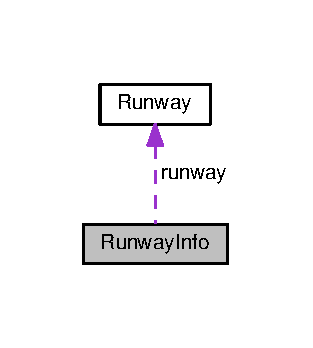
\includegraphics[width=150pt]{structRunwayInfo__coll__graph}
\end{center}
\end{figure}
\subsection*{Public Attributes}
\begin{DoxyCompactItemize}
\item 
\hyperlink{classRunway}{Runway} $\ast$ \hyperlink{structRunwayInfo_a7c0479aadb72e81995b66406971321c3}{runway}
\item 
int \hyperlink{structRunwayInfo_a3e3056a401843e8db5c9a8c08a1a692e}{arriving\+Planes}
\item 
int \hyperlink{structRunwayInfo_afc7873501db8d18cd37dead150a3ecb3}{departing\+Planes}
\end{DoxyCompactItemize}


\subsection{Detailed Description}
Struct containing info about a runway 

\subsection{Member Data Documentation}
\index{Runway\+Info@{Runway\+Info}!arriving\+Planes@{arriving\+Planes}}
\index{arriving\+Planes@{arriving\+Planes}!Runway\+Info@{Runway\+Info}}
\subsubsection[{\texorpdfstring{arriving\+Planes}{arrivingPlanes}}]{\setlength{\rightskip}{0pt plus 5cm}int Runway\+Info\+::arriving\+Planes}\hypertarget{structRunwayInfo_a3e3056a401843e8db5c9a8c08a1a692e}{}\label{structRunwayInfo_a3e3056a401843e8db5c9a8c08a1a692e}
Arriving planes at taxipoint of runway \index{Runway\+Info@{Runway\+Info}!departing\+Planes@{departing\+Planes}}
\index{departing\+Planes@{departing\+Planes}!Runway\+Info@{Runway\+Info}}
\subsubsection[{\texorpdfstring{departing\+Planes}{departingPlanes}}]{\setlength{\rightskip}{0pt plus 5cm}int Runway\+Info\+::departing\+Planes}\hypertarget{structRunwayInfo_afc7873501db8d18cd37dead150a3ecb3}{}\label{structRunwayInfo_afc7873501db8d18cd37dead150a3ecb3}
Departing planes at taxipoint of runway \index{Runway\+Info@{Runway\+Info}!runway@{runway}}
\index{runway@{runway}!Runway\+Info@{Runway\+Info}}
\subsubsection[{\texorpdfstring{runway}{runway}}]{\setlength{\rightskip}{0pt plus 5cm}{\bf Runway}$\ast$ Runway\+Info\+::runway}\hypertarget{structRunwayInfo_a7c0479aadb72e81995b66406971321c3}{}\label{structRunwayInfo_a7c0479aadb72e81995b66406971321c3}
The runway 

The documentation for this struct was generated from the following file\+:\begin{DoxyCompactItemize}
\item 
/home/max/\+C\+Lion\+Projects/\+Project\+Vliegveld/headers/Graphics.\+h\end{DoxyCompactItemize}

\hypertarget{classSystem}{}\section{System Class Reference}
\label{classSystem}\index{System@{System}}


\+: Main class, controls the simulation.  




{\ttfamily \#include $<$System.\+h$>$}

\subsection*{Public Member Functions}
\begin{DoxyCompactItemize}
\item 
\hyperlink{classSystem_a8b60d099be14345558de236d2fbc76ba}{System} (const \hyperlink{classInput}{Input} \&input, std\+::ostream \&atc, const \hyperlink{classTime}{Time} \&end)
\item 
\hyperlink{classSystem_a3be70bb338e3f062f821173fd15680d0}{$\sim$\+System} ()
\item 
void \hyperlink{classSystem_a1e6b24f8ed92dac6ce380b91268976b7}{run} (std\+::ostream \&log, const std\+::string \&impression\+Name=\char`\"{}../output/impressions/impression\char`\"{}, const std\+::string \&ini\+Name=\char`\"{}../output/ini/graphics\char`\"{})
\item 
void \hyperlink{classSystem_a62d81f9e0abc880c57972a491df4fb2e}{info} (std\+::ostream \&out)
\item 
void \hyperlink{classSystem_a779e7d437efa57c0268943dde52c6336}{generate\+Images} (\hyperlink{classTime}{Time} start, \hyperlink{classTime}{Time} end)
\item 
bool \hyperlink{classSystem_abae43adfa434ace30ef85c69a7842289}{simulation\+Finished} () const 
\item 
\hyperlink{classAirport}{Airport} $\ast$ \hyperlink{classSystem_a8cd2a9b13cdbcf30f801e46cf8284800}{get\+Airport} () const 
\item 
\hyperlink{classATC}{A\+TC} $\ast$ \hyperlink{classSystem_aae418c2545087b63188f4a4ffb2e9d15}{get\+A\+TC} () const 
\item 
std\+::vector$<$ \hyperlink{classFlightPlan}{Flight\+Plan} $\ast$ $>$ \hyperlink{classSystem_ae2f5fb3771a2d924215ca8dbd15b89ed}{get\+Flight\+Plans} () const 
\item 
bool \hyperlink{classSystem_af3eece83ba2d92a4a6b6c186d427c556}{properly\+Initialized} () const 
\end{DoxyCompactItemize}


\subsection{Detailed Description}
\+: Main class, controls the simulation. 

\subsection{Constructor \& Destructor Documentation}
\index{System@{System}!System@{System}}
\index{System@{System}!System@{System}}
\subsubsection[{\texorpdfstring{System(const Input \&input, std\+::ostream \&atc, const Time \&end)}{System(const Input &input, std::ostream &atc, const Time &end)}}]{\setlength{\rightskip}{0pt plus 5cm}System\+::\+System (
\begin{DoxyParamCaption}
\item[{const {\bf Input} \&}]{input, }
\item[{std\+::ostream \&}]{atc, }
\item[{const {\bf Time} \&}]{end}
\end{DoxyParamCaption}
)}\hypertarget{classSystem_a8b60d099be14345558de236d2fbc76ba}{}\label{classSystem_a8b60d099be14345558de236d2fbc76ba}
Constructor ~\newline
 R\+E\+Q\+U\+I\+RE(!input.get\+Airports().empty(), \char`\"{}\+There has to be an airport in the input to start the simulation\char`\"{}); ~\newline
 E\+N\+S\+U\+RE(\hyperlink{classSystem_af3eece83ba2d92a4a6b6c186d427c556}{properly\+Initialized()}, \char`\"{}constructor must end in properly\+Initialized state\char`\"{}); 
\begin{DoxyParams}{Parameters}
{\em input} & the input of the simulation \\
\hline
{\em atc} & the stream where atc messages will be written to \\
\hline
{\em end} & the ending time of the simulation \\
\hline
\end{DoxyParams}
\index{System@{System}!````~System@{$\sim$\+System}}
\index{````~System@{$\sim$\+System}!System@{System}}
\subsubsection[{\texorpdfstring{$\sim$\+System()}{~System()}}]{\setlength{\rightskip}{0pt plus 5cm}System\+::$\sim$\+System (
\begin{DoxyParamCaption}
{}
\end{DoxyParamCaption}
)}\hypertarget{classSystem_a3be70bb338e3f062f821173fd15680d0}{}\label{classSystem_a3be70bb338e3f062f821173fd15680d0}
Destructor 

\subsection{Member Function Documentation}
\index{System@{System}!generate\+Images@{generate\+Images}}
\index{generate\+Images@{generate\+Images}!System@{System}}
\subsubsection[{\texorpdfstring{generate\+Images(\+Time start, Time end)}{generateImages(Time start, Time end)}}]{\setlength{\rightskip}{0pt plus 5cm}void System\+::generate\+Images (
\begin{DoxyParamCaption}
\item[{{\bf Time}}]{start, }
\item[{{\bf Time}}]{end}
\end{DoxyParamCaption}
)}\hypertarget{classSystem_a779e7d437efa57c0268943dde52c6336}{}\label{classSystem_a779e7d437efa57c0268943dde52c6336}
Generates the images from the start time until the end time, with the use of ~\newline
 the generated ini files and the graphics engine. ~\newline
 R\+E\+Q\+U\+I\+RE(this-\/$>$\hyperlink{classSystem_af3eece83ba2d92a4a6b6c186d427c556}{properly\+Initialized()}, \char`\"{}\+System was\textquotesingle{}t initialized when calling generate\+Images\char`\"{}); 
\begin{DoxyParams}{Parameters}
{\em start} & time of first image \\
\hline
{\em end} & time of last image, not included \\
\hline
\end{DoxyParams}
\index{System@{System}!get\+Airport@{get\+Airport}}
\index{get\+Airport@{get\+Airport}!System@{System}}
\subsubsection[{\texorpdfstring{get\+Airport() const }{getAirport() const }}]{\setlength{\rightskip}{0pt plus 5cm}{\bf Airport} $\ast$ System\+::get\+Airport (
\begin{DoxyParamCaption}
{}
\end{DoxyParamCaption}
) const}\hypertarget{classSystem_a8cd2a9b13cdbcf30f801e46cf8284800}{}\label{classSystem_a8cd2a9b13cdbcf30f801e46cf8284800}
Getter for the airport in the simulation ~\newline
 R\+E\+Q\+U\+I\+RE(this-\/$>$\hyperlink{classSystem_af3eece83ba2d92a4a6b6c186d427c556}{properly\+Initialized()}, \char`\"{}\+System was\textquotesingle{}t initialized when calling get\+Airport\char`\"{}); \begin{DoxyReturn}{Returns}
\+: airport in the simulation 
\end{DoxyReturn}
\index{System@{System}!get\+A\+TC@{get\+A\+TC}}
\index{get\+A\+TC@{get\+A\+TC}!System@{System}}
\subsubsection[{\texorpdfstring{get\+A\+T\+C() const }{getATC() const }}]{\setlength{\rightskip}{0pt plus 5cm}{\bf A\+TC} $\ast$ System\+::get\+A\+TC (
\begin{DoxyParamCaption}
{}
\end{DoxyParamCaption}
) const}\hypertarget{classSystem_aae418c2545087b63188f4a4ffb2e9d15}{}\label{classSystem_aae418c2545087b63188f4a4ffb2e9d15}
Getter for the air traffic control in the simulation ~\newline
 R\+E\+Q\+U\+I\+RE(this-\/$>$\hyperlink{classSystem_af3eece83ba2d92a4a6b6c186d427c556}{properly\+Initialized()}, \char`\"{}\+System was\textquotesingle{}t initialized when calling get\+A\+T\+C\char`\"{}); \begin{DoxyReturn}{Returns}
\+: \hyperlink{classATC}{A\+TC} in the simulation 
\end{DoxyReturn}
\index{System@{System}!get\+Flight\+Plans@{get\+Flight\+Plans}}
\index{get\+Flight\+Plans@{get\+Flight\+Plans}!System@{System}}
\subsubsection[{\texorpdfstring{get\+Flight\+Plans() const }{getFlightPlans() const }}]{\setlength{\rightskip}{0pt plus 5cm}vector$<$ {\bf Flight\+Plan} $\ast$ $>$ System\+::get\+Flight\+Plans (
\begin{DoxyParamCaption}
{}
\end{DoxyParamCaption}
) const}\hypertarget{classSystem_ae2f5fb3771a2d924215ca8dbd15b89ed}{}\label{classSystem_ae2f5fb3771a2d924215ca8dbd15b89ed}
Getter for the flight plans in the simulation ~\newline
 R\+E\+Q\+U\+I\+RE(this-\/$>$\hyperlink{classSystem_af3eece83ba2d92a4a6b6c186d427c556}{properly\+Initialized()}, "\hyperlink{classSystem}{System} was\textquotesingle{}t initialized when calling get\+Flight\+Plans); \begin{DoxyReturn}{Returns}
\+: vector of flightplans that are in the simulation 
\end{DoxyReturn}
\index{System@{System}!info@{info}}
\index{info@{info}!System@{System}}
\subsubsection[{\texorpdfstring{info(std\+::ostream \&out)}{info(std::ostream &out)}}]{\setlength{\rightskip}{0pt plus 5cm}void System\+::info (
\begin{DoxyParamCaption}
\item[{std\+::ostream \&}]{out}
\end{DoxyParamCaption}
)}\hypertarget{classSystem_a62d81f9e0abc880c57972a491df4fb2e}{}\label{classSystem_a62d81f9e0abc880c57972a491df4fb2e}
Logs information of the airports and airplanes to a text file ~\newline
 R\+E\+Q\+U\+I\+RE(this-\/$>$\hyperlink{classSystem_af3eece83ba2d92a4a6b6c186d427c556}{properly\+Initialized()}, \char`\"{}\+System was\textquotesingle{}t initialized when calling info\char`\"{}); ~\newline
 R\+E\+Q\+U\+I\+RE(f\+Airport != N\+U\+LL, \char`\"{}\+No airport in the simulation\char`\"{}); 
\begin{DoxyParams}{Parameters}
{\em out} & the ostream where the info will be written to \\
\hline
\end{DoxyParams}
\index{System@{System}!properly\+Initialized@{properly\+Initialized}}
\index{properly\+Initialized@{properly\+Initialized}!System@{System}}
\subsubsection[{\texorpdfstring{properly\+Initialized() const }{properlyInitialized() const }}]{\setlength{\rightskip}{0pt plus 5cm}bool System\+::properly\+Initialized (
\begin{DoxyParamCaption}
{}
\end{DoxyParamCaption}
) const}\hypertarget{classSystem_af3eece83ba2d92a4a6b6c186d427c556}{}\label{classSystem_af3eece83ba2d92a4a6b6c186d427c556}
Checks if the object is properly initialized \begin{DoxyReturn}{Returns}
\+: boolean indicating if object is properly initialized. 
\end{DoxyReturn}
\index{System@{System}!run@{run}}
\index{run@{run}!System@{System}}
\subsubsection[{\texorpdfstring{run(std\+::ostream \&log, const std\+::string \&impression\+Name=""../output/impressions/impression"", const std\+::string \&ini\+Name=""../output/ini/graphics"")}{run(std::ostream &log, const std::string &impressionName="../output/impressions/impression", const std::string &iniName="../output/ini/graphics")}}]{\setlength{\rightskip}{0pt plus 5cm}void System\+::run (
\begin{DoxyParamCaption}
\item[{std\+::ostream \&}]{log, }
\item[{const std\+::string \&}]{impression\+Name = {\ttfamily \char`\"{}../output/impressions/impression\char`\"{}}, }
\item[{const std\+::string \&}]{ini\+Name = {\ttfamily \char`\"{}../output/ini/graphics\char`\"{}}}
\end{DoxyParamCaption}
)}\hypertarget{classSystem_a1e6b24f8ed92dac6ce380b91268976b7}{}\label{classSystem_a1e6b24f8ed92dac6ce380b91268976b7}
Runs the complete simulation ~\newline
 R\+E\+Q\+U\+I\+RE(this-\/$>$\hyperlink{classSystem_af3eece83ba2d92a4a6b6c186d427c556}{properly\+Initialized()}, \char`\"{}\+System was\textquotesingle{}t initialized when calling run\char`\"{}); ~\newline
 R\+E\+Q\+U\+I\+RE(\hyperlink{classSystem_a8cd2a9b13cdbcf30f801e46cf8284800}{get\+Airport()} != N\+U\+LL, \char`\"{}\+No airport in the simulation.\char`\"{}); ~\newline
 R\+E\+Q\+U\+I\+RE(!simulation\+Finished(), \char`\"{}\+Simulation is already finished\char`\"{});. ~\newline
 E\+N\+S\+U\+RE(\hyperlink{classSystem_abae43adfa434ace30ef85c69a7842289}{simulation\+Finished()}, \char`\"{}\+Simulation is not finished yet, error occurred\char`\"{}); 
\begin{DoxyParams}{Parameters}
{\em log} & ostream where all the log messages will be written to \\
\hline
{\em impression\+Name} & basename of the files for the impressions \\
\hline
{\em ini\+Name} & basename of the files for the ini files \\
\hline
\end{DoxyParams}
\index{System@{System}!simulation\+Finished@{simulation\+Finished}}
\index{simulation\+Finished@{simulation\+Finished}!System@{System}}
\subsubsection[{\texorpdfstring{simulation\+Finished() const }{simulationFinished() const }}]{\setlength{\rightskip}{0pt plus 5cm}bool System\+::simulation\+Finished (
\begin{DoxyParamCaption}
{}
\end{DoxyParamCaption}
) const}\hypertarget{classSystem_abae43adfa434ace30ef85c69a7842289}{}\label{classSystem_abae43adfa434ace30ef85c69a7842289}
Checks if the simulation has ended, i.\+e. specified end time has been reached ~\newline
 R\+E\+Q\+U\+I\+RE(this-\/$>$\hyperlink{classSystem_af3eece83ba2d92a4a6b6c186d427c556}{properly\+Initialized()}, \char`\"{}\+System was\textquotesingle{}t initialized when calling simulation\+Finished\char`\"{}); \begin{DoxyReturn}{Returns}
\+: boolean indicating if the simulation is finished. 
\end{DoxyReturn}


The documentation for this class was generated from the following files\+:\begin{DoxyCompactItemize}
\item 
/home/max/\+C\+Lion\+Projects/\+Project\+Vliegveld/headers/System.\+h\item 
/home/max/\+C\+Lion\+Projects/\+Project\+Vliegveld/src/System.\+cpp\end{DoxyCompactItemize}

\hypertarget{classTime}{}\section{Time Class Reference}
\label{classTime}\index{Time@{Time}}


{\ttfamily \#include $<$Time.\+h$>$}

\subsection*{Public Member Functions}
\begin{DoxyCompactItemize}
\item 
\hyperlink{classTime_a90d3b9a3fb4516e7ccb4c60deba03807}{Time} (int hour=12, int minute=0)
\item 
\hyperlink{classTime_a8d758b905e2fda239938ae0ee320453f}{Time} (const \hyperlink{classTime}{Time} \&time)
\item 
std\+::string \hyperlink{classTime_aeeb2d2b5a624d0d78b7f5d146d0682f5}{formatted} () const 
\item 
void \hyperlink{classTime_a41c94422f10c95daab849b9c20afdeba}{advance} (int minutes=1)
\item 
void \hyperlink{classTime_a9c53c93d10be3785c85449186beb6b6a}{set\+Minute} (int minute)
\item 
int \hyperlink{classTime_a6ccac73be7aacc12410cea6b3d216357}{get\+Minute} () const 
\item 
void \hyperlink{classTime_ab77d5f9f5fa8582d23a70d418ab6a182}{set\+Hour} (int hour)
\item 
int \hyperlink{classTime_a4e9d93c2aaaac84b0a49f44184968860}{get\+Hour} () const 
\item 
bool \hyperlink{classTime_ab29d371ddb19ce156377cea159efafef}{properly\+Initialized} () const 
\item 
bool \hyperlink{classTime_adeb3173efb2cb16bf361db0204a85c7c}{operator==} (const \hyperlink{classTime}{Time} \&) const 
\item 
bool \hyperlink{classTime_aa668f56a3ee77c147e7dc76bf1ad89f1}{operator$<$} (const \hyperlink{classTime}{Time} \&) const 
\item 
\hyperlink{classTime}{Time} \& \hyperlink{classTime_a7801190e243f4b6662d7d9ebadbd342f}{operator=} (const \hyperlink{classTime}{Time} \&time)
\end{DoxyCompactItemize}


\subsection{Detailed Description}
Class that represents the time 

\subsection{Constructor \& Destructor Documentation}
\index{Time@{Time}!Time@{Time}}
\index{Time@{Time}!Time@{Time}}
\subsubsection[{\texorpdfstring{Time(int hour=12, int minute=0)}{Time(int hour=12, int minute=0)}}]{\setlength{\rightskip}{0pt plus 5cm}Time\+::\+Time (
\begin{DoxyParamCaption}
\item[{int}]{hour = {\ttfamily 12}, }
\item[{int}]{minute = {\ttfamily 0}}
\end{DoxyParamCaption}
)}\hypertarget{classTime_a90d3b9a3fb4516e7ccb4c60deba03807}{}\label{classTime_a90d3b9a3fb4516e7ccb4c60deba03807}
Constructor, sets the time ~\newline
 Defaults to 12\+:00, which is the starting point of the simulation ~\newline
 R\+E\+Q\+U\+I\+RE(minute $<$ 60 \&\& minute $>$= 0, \char`\"{}\+Minute has to be between 0 and 60\char`\"{}); ~\newline
 R\+E\+Q\+U\+I\+RE(hour $<$ 24 \&\& hour $>$= 0, \char`\"{}\+Hour has to be between 0 and 24\char`\"{}); ~\newline
 E\+N\+S\+U\+RE(\hyperlink{classTime_ab29d371ddb19ce156377cea159efafef}{properly\+Initialized()}, \char`\"{}\+Time wasn\textquotesingle{}t properly initialized after constructing.\char`\"{}); 
\begin{DoxyParams}{Parameters}
{\em hour} & the hour \\
\hline
{\em minute} & the minute \\
\hline
\end{DoxyParams}
\index{Time@{Time}!Time@{Time}}
\index{Time@{Time}!Time@{Time}}
\subsubsection[{\texorpdfstring{Time(const Time \&time)}{Time(const Time &time)}}]{\setlength{\rightskip}{0pt plus 5cm}Time\+::\+Time (
\begin{DoxyParamCaption}
\item[{const {\bf Time} \&}]{time}
\end{DoxyParamCaption}
)}\hypertarget{classTime_a8d758b905e2fda239938ae0ee320453f}{}\label{classTime_a8d758b905e2fda239938ae0ee320453f}
Copy constructor ~\newline
 E\+N\+S\+U\+RE(\hyperlink{classTime_ab29d371ddb19ce156377cea159efafef}{properly\+Initialized()}, \char`\"{}\+Time wasn\textquotesingle{}t properly initialized after constructing.\char`\"{}); 
\begin{DoxyParams}{Parameters}
{\em time} & object to be copied \\
\hline
\end{DoxyParams}


\subsection{Member Function Documentation}
\index{Time@{Time}!advance@{advance}}
\index{advance@{advance}!Time@{Time}}
\subsubsection[{\texorpdfstring{advance(int minutes=1)}{advance(int minutes=1)}}]{\setlength{\rightskip}{0pt plus 5cm}void Time\+::advance (
\begin{DoxyParamCaption}
\item[{int}]{minutes = {\ttfamily 1}}
\end{DoxyParamCaption}
)}\hypertarget{classTime_a41c94422f10c95daab849b9c20afdeba}{}\label{classTime_a41c94422f10c95daab849b9c20afdeba}
Advances the time by an amount of minutes ~\newline
 R\+E\+Q\+U\+I\+RE(\hyperlink{classTime_ab29d371ddb19ce156377cea159efafef}{properly\+Initialized()}, \char`\"{}\+Time wasn\textquotesingle{}t properly\+Initialized when calling advance\char`\"{}); ~\newline
 R\+E\+Q\+U\+I\+RE(minutes $>$= 0, \char`\"{}\+Advancing by a negative amount of minutes is not possible\char`\"{}); 
\begin{DoxyParams}{Parameters}
{\em minutes} & amount of minutes to advance \\
\hline
\end{DoxyParams}
\index{Time@{Time}!formatted@{formatted}}
\index{formatted@{formatted}!Time@{Time}}
\subsubsection[{\texorpdfstring{formatted() const }{formatted() const }}]{\setlength{\rightskip}{0pt plus 5cm}string Time\+::formatted (
\begin{DoxyParamCaption}
{}
\end{DoxyParamCaption}
) const}\hypertarget{classTime_aeeb2d2b5a624d0d78b7f5d146d0682f5}{}\label{classTime_aeeb2d2b5a624d0d78b7f5d146d0682f5}
Return the time in a formatted style like such\+: \char`\"{}13\+:45\char`\"{} ~\newline
 R\+E\+Q\+U\+I\+RE(\hyperlink{classTime_ab29d371ddb19ce156377cea159efafef}{properly\+Initialized()}, \char`\"{}\+Time wasn\textquotesingle{}t properly\+Initialized when calling formatted\char`\"{}); \begin{DoxyReturn}{Returns}
string of time 
\end{DoxyReturn}
\index{Time@{Time}!get\+Hour@{get\+Hour}}
\index{get\+Hour@{get\+Hour}!Time@{Time}}
\subsubsection[{\texorpdfstring{get\+Hour() const }{getHour() const }}]{\setlength{\rightskip}{0pt plus 5cm}int Time\+::get\+Hour (
\begin{DoxyParamCaption}
{}
\end{DoxyParamCaption}
) const}\hypertarget{classTime_a4e9d93c2aaaac84b0a49f44184968860}{}\label{classTime_a4e9d93c2aaaac84b0a49f44184968860}
Getter for the hour ~\newline
 R\+E\+Q\+U\+I\+RE(\hyperlink{classTime_ab29d371ddb19ce156377cea159efafef}{properly\+Initialized()}, \char`\"{}\+Time wasn\textquotesingle{}t properly\+Initialized when calling get\+Hour\char`\"{}); \begin{DoxyReturn}{Returns}
\+: hour 
\end{DoxyReturn}
\index{Time@{Time}!get\+Minute@{get\+Minute}}
\index{get\+Minute@{get\+Minute}!Time@{Time}}
\subsubsection[{\texorpdfstring{get\+Minute() const }{getMinute() const }}]{\setlength{\rightskip}{0pt plus 5cm}int Time\+::get\+Minute (
\begin{DoxyParamCaption}
{}
\end{DoxyParamCaption}
) const}\hypertarget{classTime_a6ccac73be7aacc12410cea6b3d216357}{}\label{classTime_a6ccac73be7aacc12410cea6b3d216357}
Getter for the minute ~\newline
 R\+E\+Q\+U\+I\+RE(\hyperlink{classTime_ab29d371ddb19ce156377cea159efafef}{properly\+Initialized()}, \char`\"{}\+Time wasn\textquotesingle{}t properly\+Initialized when calling get\+Minute\char`\"{}); \begin{DoxyReturn}{Returns}
\+: minute 
\end{DoxyReturn}
\index{Time@{Time}!operator$<$@{operator$<$}}
\index{operator$<$@{operator$<$}!Time@{Time}}
\subsubsection[{\texorpdfstring{operator$<$(const Time \&) const }{operator<(const Time &) const }}]{\setlength{\rightskip}{0pt plus 5cm}bool Time\+::operator$<$ (
\begin{DoxyParamCaption}
\item[{const {\bf Time} \&}]{time}
\end{DoxyParamCaption}
) const}\hypertarget{classTime_aa668f56a3ee77c147e7dc76bf1ad89f1}{}\label{classTime_aa668f56a3ee77c147e7dc76bf1ad89f1}
Operator$<$ overloaded, returns false if comparing with 00\+:00 \index{Time@{Time}!operator=@{operator=}}
\index{operator=@{operator=}!Time@{Time}}
\subsubsection[{\texorpdfstring{operator=(const Time \&time)}{operator=(const Time &time)}}]{\setlength{\rightskip}{0pt plus 5cm}{\bf Time} \& Time\+::operator= (
\begin{DoxyParamCaption}
\item[{const {\bf Time} \&}]{time}
\end{DoxyParamCaption}
)}\hypertarget{classTime_a7801190e243f4b6662d7d9ebadbd342f}{}\label{classTime_a7801190e243f4b6662d7d9ebadbd342f}
Assignment operator 
\begin{DoxyParams}{Parameters}
{\em time} & rhs of operator \\
\hline
\end{DoxyParams}
\begin{DoxyReturn}{Returns}
reference to this 
\end{DoxyReturn}
\index{Time@{Time}!operator==@{operator==}}
\index{operator==@{operator==}!Time@{Time}}
\subsubsection[{\texorpdfstring{operator==(const Time \&) const }{operator==(const Time &) const }}]{\setlength{\rightskip}{0pt plus 5cm}bool Time\+::operator== (
\begin{DoxyParamCaption}
\item[{const {\bf Time} \&}]{time}
\end{DoxyParamCaption}
) const}\hypertarget{classTime_adeb3173efb2cb16bf361db0204a85c7c}{}\label{classTime_adeb3173efb2cb16bf361db0204a85c7c}
Operator== overloaded \index{Time@{Time}!properly\+Initialized@{properly\+Initialized}}
\index{properly\+Initialized@{properly\+Initialized}!Time@{Time}}
\subsubsection[{\texorpdfstring{properly\+Initialized() const }{properlyInitialized() const }}]{\setlength{\rightskip}{0pt plus 5cm}bool Time\+::properly\+Initialized (
\begin{DoxyParamCaption}
{}
\end{DoxyParamCaption}
) const}\hypertarget{classTime_ab29d371ddb19ce156377cea159efafef}{}\label{classTime_ab29d371ddb19ce156377cea159efafef}
Checks if the object is properly initialized \begin{DoxyReturn}{Returns}
\+: Boolean indicating if properly initialized or not. 
\end{DoxyReturn}
\index{Time@{Time}!set\+Hour@{set\+Hour}}
\index{set\+Hour@{set\+Hour}!Time@{Time}}
\subsubsection[{\texorpdfstring{set\+Hour(int hour)}{setHour(int hour)}}]{\setlength{\rightskip}{0pt plus 5cm}void Time\+::set\+Hour (
\begin{DoxyParamCaption}
\item[{int}]{hour}
\end{DoxyParamCaption}
)}\hypertarget{classTime_ab77d5f9f5fa8582d23a70d418ab6a182}{}\label{classTime_ab77d5f9f5fa8582d23a70d418ab6a182}
Setter for the hour. ~\newline
 R\+E\+Q\+U\+I\+RE(hour $<$ 24 \&\& hour $>$= 0, \char`\"{}\+Hour has to be between 0 and 24\char`\"{}); ~\newline
 R\+E\+Q\+U\+I\+RE(\hyperlink{classTime_ab29d371ddb19ce156377cea159efafef}{properly\+Initialized()}, \char`\"{}\+Time wasn\textquotesingle{}t properly\+Initialized when calling set\+Hour\char`\"{}); 
\begin{DoxyParams}{Parameters}
{\em hour} & hour to set \\
\hline
\end{DoxyParams}
\index{Time@{Time}!set\+Minute@{set\+Minute}}
\index{set\+Minute@{set\+Minute}!Time@{Time}}
\subsubsection[{\texorpdfstring{set\+Minute(int minute)}{setMinute(int minute)}}]{\setlength{\rightskip}{0pt plus 5cm}void Time\+::set\+Minute (
\begin{DoxyParamCaption}
\item[{int}]{minute}
\end{DoxyParamCaption}
)}\hypertarget{classTime_a9c53c93d10be3785c85449186beb6b6a}{}\label{classTime_a9c53c93d10be3785c85449186beb6b6a}
Setter for the minute. ~\newline
 R\+E\+Q\+U\+I\+RE(minute $<$ 60 \&\& minute $>$= 0, \char`\"{}\+Minute has to be between 0 and 60\char`\"{}); ~\newline
 R\+E\+Q\+U\+I\+RE(\hyperlink{classTime_ab29d371ddb19ce156377cea159efafef}{properly\+Initialized()}, \char`\"{}\+Time wasn\textquotesingle{}t properly\+Initialized when calling set\+Minute\char`\"{}); 
\begin{DoxyParams}{Parameters}
{\em minute} & minute to set \\
\hline
\end{DoxyParams}


The documentation for this class was generated from the following files\+:\begin{DoxyCompactItemize}
\item 
/home/max/\+C\+Lion\+Projects/\+Project\+Vliegveld/headers/Time.\+h\item 
/home/max/\+C\+Lion\+Projects/\+Project\+Vliegveld/src/Time.\+cpp\end{DoxyCompactItemize}

%--- End generated contents ---

% Index
\backmatter
\newpage
\phantomsection
\clearemptydoublepage
\addcontentsline{toc}{chapter}{Index}
\printindex

\end{document}
